% Options for packages loaded elsewhere
\PassOptionsToPackage{unicode}{hyperref}
\PassOptionsToPackage{hyphens}{url}
%
\documentclass[
  10pt,
  letterpaper,
  DIV=11,
  numbers=noendperiod,
  twoside]{scrartcl}

\usepackage{amsmath,amssymb}
\usepackage{setspace}
\usepackage{iftex}
\ifPDFTeX
  \usepackage[T1]{fontenc}
  \usepackage[utf8]{inputenc}
  \usepackage{textcomp} % provide euro and other symbols
\else % if luatex or xetex
  \usepackage{unicode-math}
  \defaultfontfeatures{Scale=MatchLowercase}
  \defaultfontfeatures[\rmfamily]{Ligatures=TeX,Scale=1}
\fi
\usepackage{lmodern}
\ifPDFTeX\else  
    % xetex/luatex font selection
  \setmainfont[ItalicFont=EB Garamond Italic,BoldFont=EB Garamond
Bold]{EB Garamond Math}
  \setsansfont[]{Europa-Bold}
  \setmathfont[]{Garamond-Math}
\fi
% Use upquote if available, for straight quotes in verbatim environments
\IfFileExists{upquote.sty}{\usepackage{upquote}}{}
\IfFileExists{microtype.sty}{% use microtype if available
  \usepackage[]{microtype}
  \UseMicrotypeSet[protrusion]{basicmath} % disable protrusion for tt fonts
}{}
\usepackage{xcolor}
\usepackage[left=1in, right=1in, top=0.8in, bottom=0.8in,
paperheight=9.5in, paperwidth=6.5in, includemp=TRUE, marginparwidth=0in,
marginparsep=0in]{geometry}
\setlength{\emergencystretch}{3em} % prevent overfull lines
\setcounter{secnumdepth}{3}
% Make \paragraph and \subparagraph free-standing
\ifx\paragraph\undefined\else
  \let\oldparagraph\paragraph
  \renewcommand{\paragraph}[1]{\oldparagraph{#1}\mbox{}}
\fi
\ifx\subparagraph\undefined\else
  \let\oldsubparagraph\subparagraph
  \renewcommand{\subparagraph}[1]{\oldsubparagraph{#1}\mbox{}}
\fi


\providecommand{\tightlist}{%
  \setlength{\itemsep}{0pt}\setlength{\parskip}{0pt}}\usepackage{longtable,booktabs,array}
\usepackage{calc} % for calculating minipage widths
% Correct order of tables after \paragraph or \subparagraph
\usepackage{etoolbox}
\makeatletter
\patchcmd\longtable{\par}{\if@noskipsec\mbox{}\fi\par}{}{}
\makeatother
% Allow footnotes in longtable head/foot
\IfFileExists{footnotehyper.sty}{\usepackage{footnotehyper}}{\usepackage{footnote}}
\makesavenoteenv{longtable}
\usepackage{graphicx}
\makeatletter
\def\maxwidth{\ifdim\Gin@nat@width>\linewidth\linewidth\else\Gin@nat@width\fi}
\def\maxheight{\ifdim\Gin@nat@height>\textheight\textheight\else\Gin@nat@height\fi}
\makeatother
% Scale images if necessary, so that they will not overflow the page
% margins by default, and it is still possible to overwrite the defaults
% using explicit options in \includegraphics[width, height, ...]{}
\setkeys{Gin}{width=\maxwidth,height=\maxheight,keepaspectratio}
% Set default figure placement to htbp
\makeatletter
\def\fps@figure{htbp}
\makeatother

\setlength\heavyrulewidth{0ex}
\setlength\lightrulewidth{0ex}
\usepackage[automark]{scrlayer-scrpage}
\clearpairofpagestyles
\cehead{
  Brian Weatherson
  }
\cohead{
  Some Data about Citation Trends
  }
\ohead{\bfseries \pagemark}
\cfoot{}
\makeatletter
\newcommand*\NoIndentAfterEnv[1]{%
  \AfterEndEnvironment{#1}{\par\@afterindentfalse\@afterheading}}
\makeatother
\NoIndentAfterEnv{itemize}
\NoIndentAfterEnv{enumerate}
\NoIndentAfterEnv{description}
\NoIndentAfterEnv{quote}
\NoIndentAfterEnv{equation}
\NoIndentAfterEnv{longtable}
\NoIndentAfterEnv{abstract}
\renewenvironment{abstract}
 {\vspace{-1.25cm}
 \quotation\small\noindent\rule{\linewidth}{.5pt}\par\smallskip
 \noindent }
 {\par\noindent\rule{\linewidth}{.5pt}\endquotation}
\KOMAoption{captions}{tableheading}
\makeatletter
\@ifpackageloaded{caption}{}{\usepackage{caption}}
\AtBeginDocument{%
\ifdefined\contentsname
  \renewcommand*\contentsname{Table of contents}
\else
  \newcommand\contentsname{Table of contents}
\fi
\ifdefined\listfigurename
  \renewcommand*\listfigurename{List of Figures}
\else
  \newcommand\listfigurename{List of Figures}
\fi
\ifdefined\listtablename
  \renewcommand*\listtablename{List of Tables}
\else
  \newcommand\listtablename{List of Tables}
\fi
\ifdefined\figurename
  \renewcommand*\figurename{Figure}
\else
  \newcommand\figurename{Figure}
\fi
\ifdefined\tablename
  \renewcommand*\tablename{Table}
\else
  \newcommand\tablename{Table}
\fi
}
\@ifpackageloaded{float}{}{\usepackage{float}}
\floatstyle{ruled}
\@ifundefined{c@chapter}{\newfloat{codelisting}{h}{lop}}{\newfloat{codelisting}{h}{lop}[chapter]}
\floatname{codelisting}{Listing}
\newcommand*\listoflistings{\listof{codelisting}{List of Listings}}
\makeatother
\makeatletter
\makeatother
\makeatletter
\@ifpackageloaded{caption}{}{\usepackage{caption}}
\@ifpackageloaded{subcaption}{}{\usepackage{subcaption}}
\makeatother
\ifLuaTeX
  \usepackage{selnolig}  % disable illegal ligatures
\fi
\usepackage{bookmark}

\IfFileExists{xurl.sty}{\usepackage{xurl}}{} % add URL line breaks if available
\urlstyle{same} % disable monospaced font for URLs
\hypersetup{
  pdftitle={Some Data about Citation Trends},
  pdfauthor={Brian Weatherson},
  hidelinks,
  pdfcreator={LaTeX via pandoc}}

\title{Some Data about Citation Trends}
\author{Brian Weatherson}
\date{2024}

\begin{document}
\maketitle
\begin{abstract}
In the future I plan to write something substantive about trends in
citations in philosophy journals. This is a presentation of some of the
underlying data, with some small remarks about the big picture trends.
\end{abstract}

\setstretch{1.1}
I recently downloaded citation data for 100 philosophy journals from Web
of Science. This note presents some of the data about trends in citation
patterns since 1976. My main interest here is in seeing which changes
there have been in what was cited over time, but there are lots of
interesting nuggets. Later I'll write a real paper actually going into
what some of the data mean, but for now I'm just presenting it for
public consumption.

\section{Methodology}\label{methodology}

\subsection{The Articles Being
Studied}\label{the-articles-being-studied}

Via the University of Michigan, I got the latest available database for
Web of Science circa January 2024. I created a file of every citation
where both the citing article and the cited article were from one of the
100 journals in Table~\ref{tbl-list-of-journals}, in the years that they
were indexed by Web of Science.

\begin{longtable}[]{@{}
  >{\raggedright\arraybackslash}p{(\columnwidth - 6\tabcolsep) * \real{0.7702}}
  >{\raggedleft\arraybackslash}p{(\columnwidth - 6\tabcolsep) * \real{0.0559}}
  >{\raggedleft\arraybackslash}p{(\columnwidth - 6\tabcolsep) * \real{0.0683}}
  >{\raggedleft\arraybackslash}p{(\columnwidth - 6\tabcolsep) * \real{0.1056}}@{}}

\caption{\label{tbl-list-of-journals}The journals included in this
study}

\tabularnewline

\toprule\noalign{}
\begin{minipage}[b]{\linewidth}\raggedright
Journal
\end{minipage} & \begin{minipage}[b]{\linewidth}\raggedleft
Articles
\end{minipage} & \begin{minipage}[b]{\linewidth}\raggedleft
First Year
\end{minipage} & \begin{minipage}[b]{\linewidth}\raggedleft
Most Recent Year
\end{minipage} \\
\midrule\noalign{}
\endhead
\bottomrule\noalign{}
\endlastfoot
Acta Philosophica & 211 & 2009 & 2022 \\
American Philosophical Quarterly & 1636 & 1968 & 2021 \\
Analysis & 2615 & 1975 & 2022 \\
Analytic Philosophy & 169 & 2016 & 2022 \\
Archiv Fur Geschichte Der Philosophie & 676 & 1975 & 2022 \\
Australasian Journal Of Philosophy & 1683 & 1975 & 2022 \\
Biology \& Philosophy & 1117 & 1988 & 2022 \\
British Journal For The History Of Philosophy & 760 & 2007 & 2022 \\
British Journal For The Philosophy Of Science & 1328 & 1969 & 2022 \\
British Journal Of Aesthetics & 1369 & 1975 & 2022 \\
Canadian Journal Of Philosophy & 1497 & 1975 & 2022 \\
Croatian Journal Of Philosophy & 329 & 2007 & 2022 \\
Dialogue-Canadian Philosophical Review & 1464 & 1975 & 2022 \\
Economics And Philosophy & 116 & 2003 & 2022 \\
Episteme-A Journal Of Individual And Social Epistemology & 551 & 2005 &
2022 \\
Ergo-An Open Access Journal Of Philosophy & 213 & 2016 & 2021 \\
Erkenntnis & 1744 & 2000 & 2022 \\
Ethical Theory And Moral Practice & 854 & 2008 & 2022 \\
Ethics & 1347 & 1968 & 2022 \\
European Journal For Philosophy Of Science & 449 & 2011 & 2022 \\
European Journal Of Philosophy & 914 & 1998 & 2022 \\
Heythrop Journal-A Quarterly Review Of Philosophy And Theology & 792 &
1975 & 2014 \\
History And Philosophy Of Logic & 475 & 1992 & 2022 \\
Hume Studies & 111 & 2010 & 2022 \\
Hypatia-A Journal Of Feminist Philosophy & 607 & 2009 & 2022 \\
Inquiry-An Interdisciplinary Journal Of Philosophy & 1699 & 1968 &
2022 \\
International Journal For Philosophy Of Religion & 1098 & 1975 & 2022 \\
International Philosophical Quarterly & 1350 & 1968 & 2022 \\
Journal Of Aesthetics And Art Criticism & 1473 & 1975 & 2022 \\
Journal Of Applied Philosophy & 607 & 2006 & 2022 \\
Journal Of Chinese Philosophy & 1234 & 1973 & 2022 \\
Journal Of Consciousness Studies & 1356 & 2000 & 2022 \\
Journal Of Indian Philosophy & 1034 & 1975 & 2022 \\
Journal Of Medical Ethics & 270 & 1975 & 2022 \\
Journal Of Moral Philosophy & 347 & 2005 & 2022 \\
Journal Of Philosophical Logic & 1411 & 1972 & 2022 \\
Journal Of Philosophical Research & 508 & 2005 & 2022 \\
Journal Of Philosophy & 1649 & 1968 & 2022 \\
Journal Of Political Philosophy & 282 & 2003 & 2022 \\
Journal Of Social Philosophy & 481 & 2008 & 2022 \\
Journal Of The American Philosophical Association & 306 & 2015 & 2022 \\
Journal Of The History Of Ideas & 1669 & 1968 & 2022 \\
Journal Of The History Of Philosophy & 1083 & 1975 & 2022 \\
Journal Of Value Inquiry & 1358 & 1980 & 2022 \\
Kant-Studien & 1068 & 1975 & 2022 \\
Kantian Review & 293 & 2010 & 2022 \\
Kennedy Institute Of Ethics Journal & 551 & 1995 & 2022 \\
Law And Philosophy & 208 & 2003 & 2022 \\
Logique Et Analyse & 339 & 2007 & 2021 \\
Metaphilosophy & 1470 & 1975 & 2022 \\
Midwest Studies In Philosophy & 107 & 1984 & 1988 \\
Mind & 1579 & 1968 & 2022 \\
Mind \& Language & 155 & 2003 & 2022 \\
Minds And Machines & 192 & 2003 & 2022 \\
Monist & 1739 & 1968 & 2022 \\
Notre Dame Journal Of Formal Logic & 424 & 2009 & 2022 \\
Nous & 1886 & 1975 & 2022 \\
Pacific Philosophical Quarterly & 1190 & 1980 & 2022 \\
Philosophers Imprint & 353 & 2010 & 2022 \\
Philosophia & 2050 & 1975 & 2022 \\
Philosophia Mathematica & 221 & 2008 & 2022 \\
Philosophical Explorations & 353 & 2008 & 2022 \\
Philosophical Forum & 802 & 1971 & 2022 \\
Philosophical Investigations & 680 & 1983 & 2023 \\
Philosophical Papers & 225 & 2009 & 2022 \\
Philosophical Perspectives & 275 & 2007 & 2022 \\
Philosophical Psychology & 291 & 2003 & 2022 \\
Philosophical Quarterly & 1341 & 1975 & 2022 \\
Philosophical Review & 717 & 1968 & 2022 \\
Philosophical Studies & 4980 & 1968 & 2022 \\
Philosophical Topics & 106 & 1981 & 1986 \\
Philosophy & 1696 & 1968 & 2023 \\
Philosophy \& Public Affairs & 698 & 1971 & 2022 \\
Philosophy And Phenomenological Research & 2792 & 1968 & 2022 \\
Philosophy And Rhetoric & 886 & 1975 & 2022 \\
Philosophy Compass & 541 & 2015 & 2023 \\
Philosophy East \& West & 1461 & 1968 & 2022 \\
Philosophy Of Science & 2716 & 1968 & 2022 \\
Philosophy Of The Social Sciences & 920 & 1975 & 2023 \\
Phronesis-A Journal For Ancient Philosophy & 743 & 1975 & 2022 \\
Politics Philosophy \& Economics & 197 & 2008 & 2023 \\
Ratio & 566 & 1974 & 2022 \\
Ratio-New Series & 474 & 1974 & 2004 \\
Review Of Metaphysics & 1143 & 1968 & 2022 \\
Review Of Symbolic Logic & 535 & 2008 & 2022 \\
Russell-The Journal Of The Bertrand Russell Archives & 246 & 1975 &
2003 \\
Russell-The Journal Of The Bertrand Russell Studies & 133 & 1984 &
2022 \\
Social Philosophy \& Policy & 893 & 1983 & 2021 \\
South African Journal Of Philosophy & 726 & 1987 & 2022 \\
Southern Journal Of Philosophy & 1899 & 1976 & 2022 \\
Southwestern Journal Of Philosophy & 422 & 1970 & 1980 \\
Studia Logica & 666 & 2010 & 2022 \\
Studies In History And Philosophy Of Science & 1660 & 1974 & 2022 \\
Studies In History And Philosophy Of Science Part C-Studies In History
And Philosophy Of Biological And Biomedical Sciences & 141 & 2017 &
2020 \\
Synthese & 6936 & 1968 & 2022 \\
Theoria-A Swedish Journal Of Philosophy & 395 & 2007 & 2022 \\
Thought-A Journal Of Philosophy & 188 & 2016 & 2021 \\
Topoi-An International Review Of Philosophy & 1113 & 1982 & 2022 \\
Transactions Of The Charles S Peirce Society & 1132 & 1975 & 2022 \\
Utilitas & 360 & 2009 & 2022 \\

\end{longtable}

Of course the first year isn't the first year the journal started
publishing; it's when Web of Science started indexing them. And the last
year isn't when they ceased publishing; it's the most recent year
indexed. Web of Science is very slow at adding journals, and at adding
volumes. But it is, as far as I've found, pretty accurate within what it
adds.

One big exception to this is that it's never really understood how to
handle the `supplements' to \emph{Noûs}, i.e., \emph{Philosophical
Perspectives} and \emph{Philosophical Issues}. Some of these are
recorded as being their own thing, some of them are recorded as special
issues of \emph{Noûs}. In the latter case, the citations often only
start being tracked several years after publication, and the
bibliographic information is spotty. This affects some of what we see
below.

Because Web of Science keeps adding journals, and journals keep getting
larger, the number of articles in this study keeps going up. The only
downward pressure comes from the fact that some journals haven't been
indexed for 2022 or even, in some cases, 2021.
Figure~\ref{fig-number-of-articles-by-year} shows how many articles each
year are in the study.

\begin{figure}

\centering{

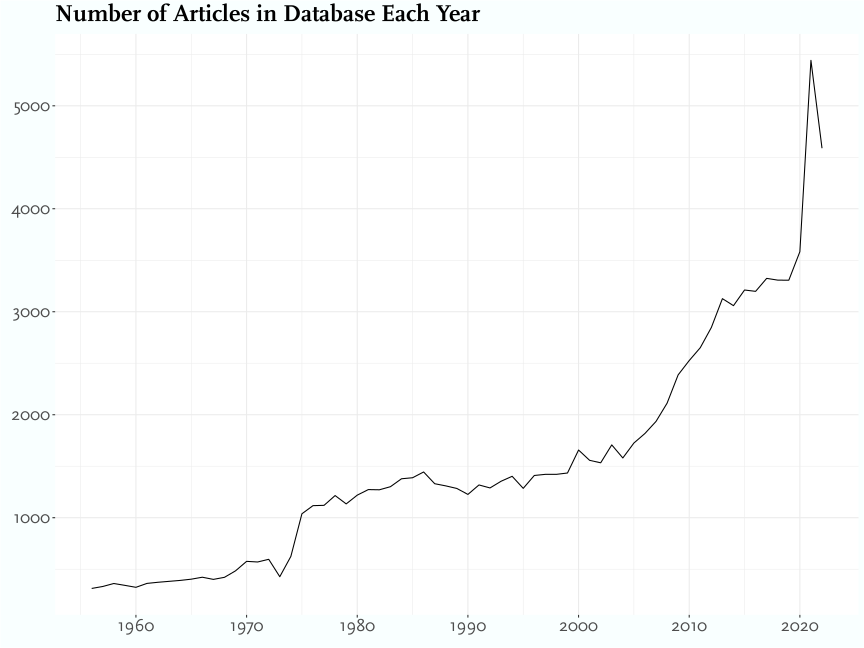
\includegraphics{citations_files/figure-pdf/fig-number-of-articles-by-year-1.pdf}

}

\caption{\label{fig-number-of-articles-by-year}Number of articles in the
study each year}

\end{figure}%

On top of that, citation practices have changed and people now cite much
more widely than they used to. So the number of citations recorded each
year (to articles since 1976 indexed in these 100 journals), has risen
rather dramatically, as shown in
Figure~\ref{fig-number-of-citations-by-year}.

\begin{figure}

\centering{

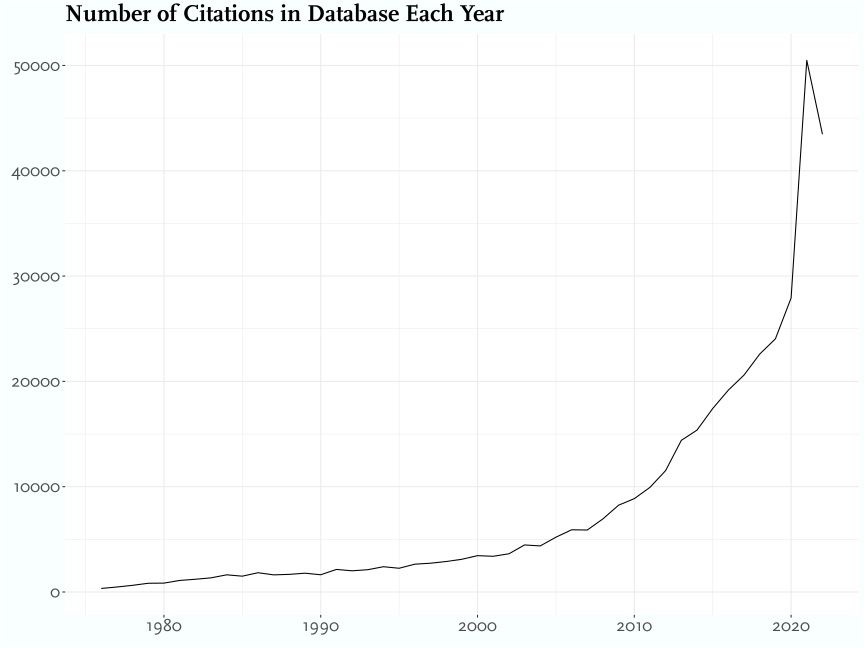
\includegraphics{citations_files/figure-pdf/fig-number-of-citations-by-year-1.pdf}

}

\caption{\label{fig-number-of-citations-by-year}Number of citations to
articles in the study each year}

\end{figure}%

On the other hand, since the overwhelming majority of citations are to
articles published earlier than the citing article, a larger number of
citations in total might be consistent with fewer citations per article
available to be cited. If we somewhat arbitrarily set the universe of
possible cited papers to be the set of papers with the same publication
date as the citing article or earlier,
Figure~\ref{fig-average-of-citations-by-year} shows how often the
average paper was cited each year (in these 100 journals).

\begin{figure}

\centering{

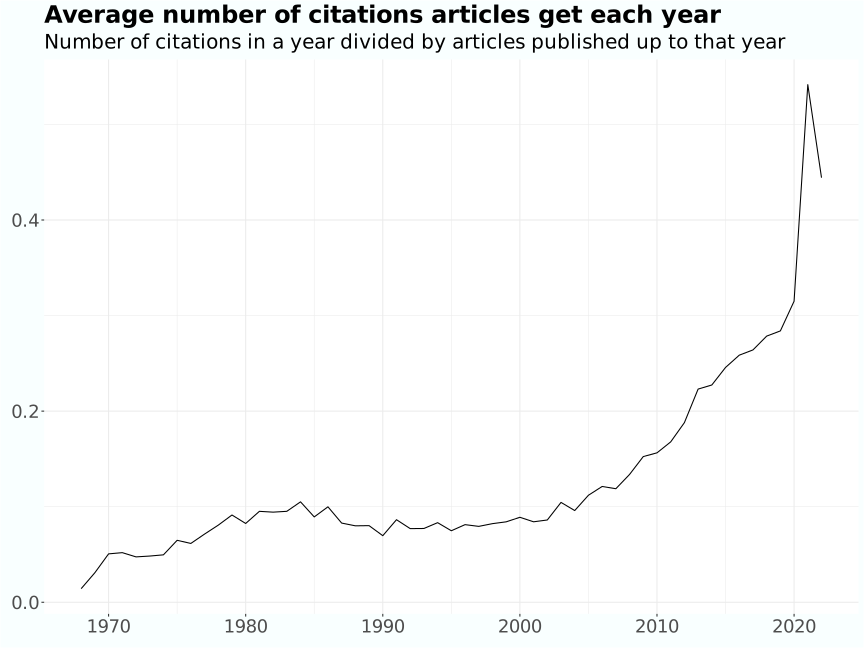
\includegraphics{citations_files/figure-pdf/fig-average-of-citations-by-year-1.pdf}

}

\caption{\label{fig-average-of-citations-by-year}Average number of
citations per available article in each each year}

\end{figure}%

Between about 1978 and 2004, the different forces are roughly balanced.
There are more papers, and each paper cites more often, but there are
more papers available to be cited, and the mean stays at about 0.1. (Of
course articles do get cited outside of journals indexed in Web of
Science, but it's still a bit humbling to realise that's the historical
average, even if one gets published in a journal as good as one of
these.) But then the forces pushing this number up take over. This is
important context for a lot of the graphs below, where the typical
article will have a graph of citations per year that looks a bit like
this.

\subsection{The Focus}\label{the-focus}

For each year up to 2015, I made three lists. (After 2015 the citation
data is all too new to be particularly useful I think.) First, a list of
the articles published that year sorted by how many times they are
cited. Second, the same list sorted by how many times they are cited in
the first ten years after publication. Third, the same list sorted by
how many times they are cited in the last ten years of the study. As we
get closer to the present, the three lists overlap considerably. Given
how many of the citations come from the last few years, the first and
third lists overlap a lot in any case.

Then I found the largest \emph{n} such that taking the top \emph{n} from
those three lists gave me nine total articles per year. (If forced to
choose, I chose the articles with the most total citations.) So we got a
mix largely of highly cited articles, and articles that were highly
cited soon after publication. With nine articles each year, and forty
years between 1976 and 2015, we end up with 360 articles. I won't list
them here because they are all listed in one way or other below.

The 360 articles are, for better and for worse, a pretty representative
sample of what was happening in those journals, and in particular what
was being widely talked about in those journals. They wouldn't match up
with my list of the best 360 articles from those forty years, or I
suspect anyone else's list of the best 360 articles. But I do think they
are an interesting model of the field as it was across those years.

It was not a surprise that the famously high prestige journals have the
bulk of these articles. But there was more variation within the list
than some may have expected, as we see in
Table~\ref{tbl-journals-in-main-bib}.

\begin{longtable}[]{@{}lr@{}}

\caption{\label{tbl-journals-in-main-bib}Which journals the 360 articles
appeared in.}

\tabularnewline

\toprule\noalign{}
Journal & Articles \\
\midrule\noalign{}
\endhead
\bottomrule\noalign{}
\endlastfoot
Journal Of Philosophy & 54 \\
Philosophical Review & 42 \\
Philosophical Studies & 33 \\
Noûs & 30 \\
Philosophy And Phenomenological Research & 23 \\
Mind & 22 \\
Philosophy Of Science & 21 \\
Ethics & 17 \\
Synthese & 13 \\
Philosophy \& Public Affairs & 12 \\
Philosophical Quarterly & 11 \\
American Philosophical Quarterly & 10 \\
Analysis & 10 \\
Australasian Journal Of Philosophy & 9 \\
British Journal For The Philosophy Of Science & 7 \\
Journal Of Philosophical Logic & 7 \\
Pacific Philosophical Quarterly & 5 \\
Monist & 4 \\
Philosophers Imprint & 3 \\
Biology \& Philosophy & 2 \\
Canadian Journal Of Philosophy & 2 \\
Erkenntnis & 2 \\
Hypatia-A Journal Of Feminist Philosophy & 2 \\
Inquiry-An Interdisciplinary Journal Of Philosophy & 2 \\
Journal Of The American Philosophical Association & 2 \\
Midwest Studies In Philosophy & 2 \\
Philosophical Perspectives & 2 \\
Ratio-New Series & 2 \\
Studies In History And Philosophy Of Science & 2 \\
European Journal Of Philosophy & 1 \\
Metaphilosophy & 1 \\
Mind \& Language & 1 \\
Philosophical Psychology & 1 \\
Philosophy Compass & 1 \\
Review Of Metaphysics & 1 \\
Review Of Symbolic Logic & 1 \\

\end{longtable}

A bit under half the articles (171 out of 360) are in the journals
widely taken to be the big five: Journal of Philosophy, Philosophical
Review, Mind, Noûs, and Philosophy and Phenomenological Research. If we
restrict attention to just the last ten years, and look at which
articles from 2006 to 2015 are widely cited in this sense, there is even
more variation, as shown in Table~\ref{tbl-recent-journals-in-main-bib}.

\begin{longtable}[]{@{}lr@{}}

\caption{\label{tbl-recent-journals-in-main-bib}Which journals the most
recent 90 articles appeared in.}

\tabularnewline

\toprule\noalign{}
Journal & Articles \\
\midrule\noalign{}
\endhead
\bottomrule\noalign{}
\endlastfoot
Philosophical Studies & 11 \\
Philosophy And Phenomenological Research & 9 \\
Journal Of Philosophy & 8 \\
Noûs & 8 \\
Philosophical Review & 7 \\
Synthese & 7 \\
Mind & 5 \\
Philosophical Quarterly & 4 \\
British Journal For The Philosophy Of Science & 3 \\
Philosophers Imprint & 3 \\
Biology \& Philosophy & 2 \\
Erkenntnis & 2 \\
Ethics & 2 \\
Hypatia-A Journal Of Feminist Philosophy & 2 \\
Inquiry-An Interdisciplinary Journal Of Philosophy & 2 \\
Journal Of The American Philosophical Association & 2 \\
Pacific Philosophical Quarterly & 2 \\
Philosophical Perspectives & 2 \\
Philosophy Of Science & 2 \\
Australasian Journal Of Philosophy & 1 \\
European Journal Of Philosophy & 1 \\
Journal Of Philosophical Logic & 1 \\
Mind \& Language & 1 \\
Monist & 1 \\
Philosophy Compass & 1 \\
Review Of Symbolic Logic & 1 \\

\end{longtable}

The big five still cover over 40\% of the articles, but the journal with
the most representatives is \emph{Philosophical Studies}. Now part of
that is that it publishes so many articles, but lots of journals publish
lots of articles without having this much impact.

\subsection{Short Observations}\label{short-observations}

In longer work I plan to make a lot of notes about the data that's
presented here. But for now I'll just note a few things about changes in
the citation patterns over the last forty years.

There are a few reasons that articles might be widely cited immediately
after they come out, and then not so widely cited after a few years.

\begin{itemize}
\tightlist
\item
  The article might get turned into a book, and people simply cite the
  book. You can see that happening in the data below with articles by
  Ted Sider, by John MacFarlane, and by Timothy Williamson, for example.
  It's not part of this study, but not that many people cite Lewis's
  1973 paper on counterfactuals, because they mostly cite his 1973 book
  on counterfactuals. But books don't always soak up the citations that
  papers would otherwise have received. People didn't take the
  discussion of natural properties in \emph{Plurality} to mean they
  should stop citing ``New Work''. Jason Stanley and Timothy
  Williamson's paper on knowing how gets more citations after Stanley's
  book on know how comes out. Still, it is one relatively mundane reason
  that a paper doesn't get much attention.
\item
  The article might simply get superseded. This can happen with
  technical papers in particular. If a paper has some useful technical
  developments, but they are incorporated into later and better work,
  perhaps people just stop citing the earlier work.
\item
  If the article is a negative article, it might simply convince people
  not to pay attention to a particular debate. This does happen a bit; I
  think Karen Bennett's 2003 paper on the causal exclusion problem is
  more influential than you see in the citation data, simply because it
  settled various problems convincingly enough to convince people to
  write about other things. Bennett's paper does get a pretty good
  number of citations, but even so I think it gets less than some less
  influential papers. But this kind of phenomena, where papers lose
  citations because they convince people to move on, isn't that common.
  People didn't stop citing \emph{Sense and Sensibilia} when they
  decided sense-data theory had been a mistake.
\end{itemize}

But sometimes articles stop getting cited because the philosophical
fashion moves on, and they seem like a relic of an earlier age. You
really see this in the data below with articles about
\textbf{supervenience}. Now I'm enough of an old fashioned
intensionalist to think that getting clear on the different kinds of
supervenience is in fact a worthwhile project. But the discipline as a
whole doesn't really agree. Nobody is citing the work, especially the
early work, on different concepts of supervenience.

What would have been even more shocking to me thirty years ago is how
little attention is paid in the journals now to debates about content
externalism. That felt like the most important debate in philosophy for
so long, and now it simply isn't.

From the other direction, what has picked up the attention? There are
two important things to look at here: new topics, and topics that get
more attention now than they used to. The first one is easy: the big new
topics at the end of the data set are \textbf{conceptual engineering}
and \textbf{grounding}. The second is, to my mind, more interesting.

There are two categories of articles that stand out immediately among
the papers that are more widely cited now than when they first came out.

The biggest of these is \textbf{social philosophy}. In this I'm
including Rae Langton's 1993 article on silencing, Sally Haslanger's
2000 \emph{Noûs} article on race and gender, and Kristie Dotson's 2011
article on epistemic violence. But I'm also including things like
Michael Bratman's 1992 and 1993 articles on collective action. It's a
bit of a stretch, but one might also see the various articles on trust
that show up below (by Annette Baier, Richard Holton, and Karen Jones),
as being of the move towards more social philosophy. Philosophy in the
twentieth century was very focussed on individuals; there is much more
attention now to groups and societies.

The other category is papers on \textbf{probability}. Some papers from
the 1990s, such as Richard Foley's 1992 paper that set out the Lockean
theory of belief, and Jim Joyce's 1998 paper setting up the
accuracy-dominance approoach, are much more widely discussed now than
they were immediately after they came out.

One of my aims with this is to use the co-citation relations between
these 360 papers to find more categories, and especially categories that
are linked by more than my gut feeling that they fit together. But
that's a project for a much bigger project. The aim here is mostly to
present some data, and if anyone has ideas about how it could be used,
they should feel free to investigate them!

\section{Yearly Data}\label{yearly-data}

\subsection{1976}\label{section}

\subsubsection*{Widely Cited Articles}\label{widely-cited-articles}
\addcontentsline{toc}{subsubsection}{Widely Cited Articles}

\begin{enumerate}
\def\labelenumi{\arabic{enumi}.}
\tightlist
\item
  AI Goldman, ``Discrimination and Perceptual Knowledge'' \emph{Journal
  Of Philosophy} 73 (20): 771-791.
\item
  D Lewis, ``Probabilities of Conditionals and Conditional
  Probabilities'' \emph{Philosophical Review} 85 (3): 297-315.
\item
  D Lewis, ``Paradoxes of Time Travel'' \emph{American Philosophical
  Quarterly} 13 (2): 145-152.
\item
  M Stocker, ``Schizophrenia of Modern Ethical Theories'' \emph{Journal
  Of Philosophy} 73 (14): 453-466.
\item
  G Harman, ``Practical Reasoning'' \emph{Review Of Metaphysics} 29 (3):
  431-463.
\item
  RC Stalnaker, ``Possible Worlds'' \emph{Noûs} 10 (1): 65-75.
\item
  JM Dunn, ``Intuitive Semantics for First-Degree Entailments and
  Coupled Trees'' \emph{Philosophical Studies} 29 (3): 149-168.
\item
  WP Alston, ``Two Types of Foundationalism'' \emph{Journal Of
  Philosophy} 73 (7): 165-185.
\item
  B Loar, ``Semantics of Singular Terms'' \emph{Philosophical Studies}
  30 (6): 353-377.
\end{enumerate}

\subsubsection*{Citation Count}\label{citation-count}
\addcontentsline{toc}{subsubsection}{Citation Count}

\begin{longtable}[]{@{}lrrr@{}}

\caption{\label{tbl-citation-count-1976}Citation count for widely cited
articles from 1976.}

\tabularnewline

\toprule\noalign{}
Article & All & Early & Late \\
\midrule\noalign{}
\endhead
\bottomrule\noalign{}
\endlastfoot
Goldman & 404 & 48 & 196 \\
Lewis, Probabilities & 239 & 28 & 116 \\
Lewis, Time Travel & 174 & 12 & 110 \\
Stocker & 145 & 10 & 64 \\
Harman & 137 & 14 & 71 \\
Stalnaker & 101 & 13 & 54 \\
Dunn & 90 & 7 & 62 \\
Loar & 48 & 12 & 20 \\
Alston & 30 & 16 & 5 \\

\end{longtable}

\subsubsection*{Citation Rank}\label{citation-rank}
\addcontentsline{toc}{subsubsection}{Citation Rank}

\begin{longtable}[]{@{}lrrr@{}}

\caption{\label{tbl-citation-rank-1976}Citation rank for widely cited
articles from 1976.}

\tabularnewline

\toprule\noalign{}
Article & Overall & Early & Late \\
\midrule\noalign{}
\endhead
\bottomrule\noalign{}
\endlastfoot
Goldman & 1 & 1 & 1 \\
Lewis, Probabilities & 2 & 2 & 2 \\
Lewis, Time Travel & 3 & 6 & 3 \\
Stocker & 4 & 11 & 5 \\
Harman & 5 & 4 & 4 \\
Stalnaker & 6 & 5 & 7 \\
Dunn & 7 & 21 & 6 \\
Loar & 11 & 6 & 11 \\
Alston & 18 & 3 & 42 \\

\end{longtable}

\subsubsection*{Citation Trends}\label{citation-trends}
\addcontentsline{toc}{subsubsection}{Citation Trends}

\begin{figure}

\centering{

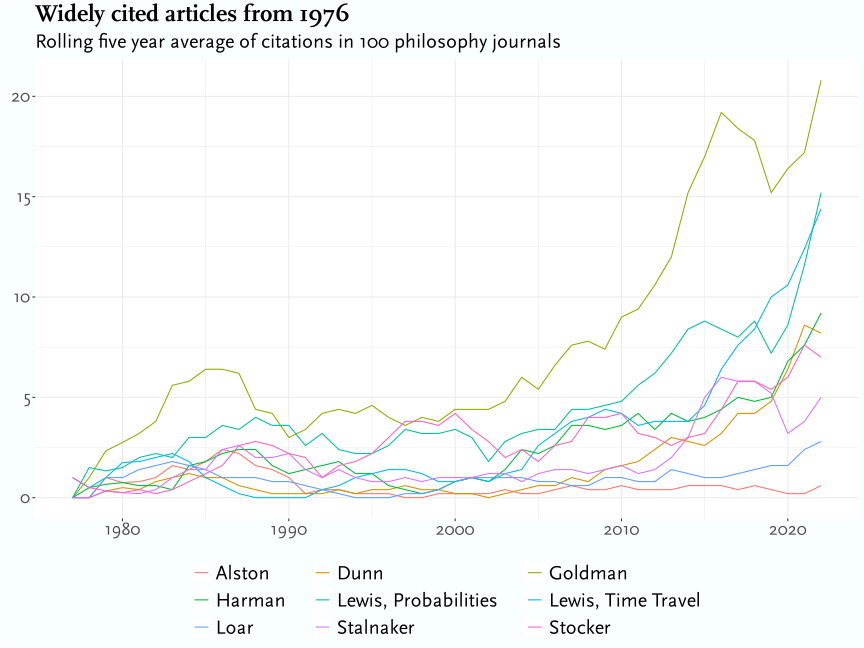
\includegraphics{citations_files/figure-pdf/fig-citation-spaghetti-1976-1.pdf}

}

\caption{\label{fig-citation-spaghetti-1976}Rolling five year average of
citation frequency for widely cited articles from 1976.}

\end{figure}%

\begin{figure}

\centering{

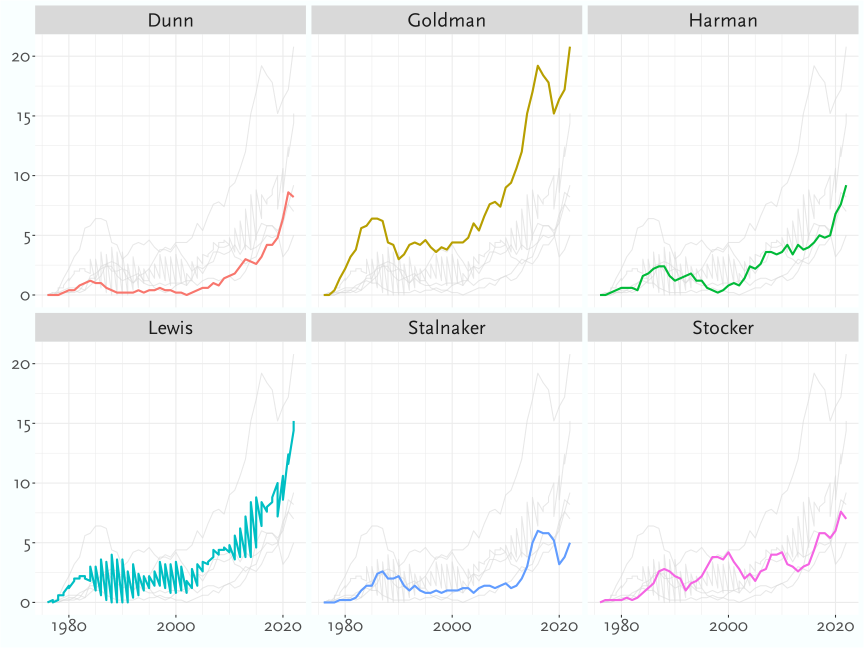
\includegraphics{citations_files/figure-pdf/fig-citation-facet-1976-1.pdf}

}

\caption{\label{fig-citation-facet-1976}Faceted version of
Figure~\ref{fig-citation-spaghetti-1976}.}

\end{figure}%

\newpage

\subsection{1977}\label{section-1}

\subsubsection*{Widely Cited Articles}\label{widely-cited-articles-1}
\addcontentsline{toc}{subsubsection}{Widely Cited Articles}

\begin{enumerate}
\def\labelenumi{\arabic{enumi}.}
\tightlist
\item
  FI Dretske, ``Laws of Nature'' \emph{Philosophy Of Science} 44 (2):
  248-268.
\item
  SL Darwall, ``Two Kinds of Respect'' \emph{Ethics} 88 (1): 36-49.
\item
  J Perry, ``Frege on Demonstratives'' \emph{Philosophical Review} 86
  (4): 474-497.
\item
  M Tooley, ``Nature of Laws'' \emph{Canadian Journal Of Philosophy} 7
  (4): 667-698.
\item
  JM Taurek, ``Should Numbers Count'' \emph{Philosophy \& Public
  Affairs} 6 (4): 293-316.
\item
  C Boorse, ``Health as a Theoretical Concept'' \emph{Philosophy Of
  Science} 44 (4): 542-573.
\item
  T Burge, ``Belief De Re'' \emph{Journal Of Philosophy} 74 (6):
  338-362.
\item
  HN Castañeda, ``Perception, Belief, and Structure of Physical Objects
  and Consciousness'' \emph{Synthese} 35 (3): 285-351.
\item
  HH Field, ``Logic, Meaning, and Conceptual Role'' \emph{Journal Of
  Philosophy} 74 (7): 379-409.
\end{enumerate}

\subsubsection*{Citation Count}\label{citation-count-1}
\addcontentsline{toc}{subsubsection}{Citation Count}

\begin{longtable}[]{@{}lrrr@{}}

\caption{\label{tbl-citation-count-1977}Citation count for widely cited
articles from 1977.}

\tabularnewline

\toprule\noalign{}
Article & All & Early & Late \\
\midrule\noalign{}
\endhead
\bottomrule\noalign{}
\endlastfoot
Dretske & 198 & 22 & 84 \\
Darwall & 190 & 3 & 135 \\
Perry & 189 & 35 & 74 \\
Tooley & 187 & 19 & 85 \\
Taurek & 142 & 10 & 76 \\
Burge & 111 & 34 & 29 \\
Boorse & 107 & 3 & 75 \\
Field & 83 & 23 & 21 \\
Castañeda & 36 & 27 & 1 \\

\end{longtable}

\subsubsection*{Citation Rank}\label{citation-rank-1}
\addcontentsline{toc}{subsubsection}{Citation Rank}

\begin{longtable}[]{@{}lrrr@{}}

\caption{\label{tbl-citation-rank-1977}Citation rank for widely cited
articles from 1977.}

\tabularnewline

\toprule\noalign{}
Article & Overall & Early & Late \\
\midrule\noalign{}
\endhead
\bottomrule\noalign{}
\endlastfoot
Dretske & 1 & 5 & 3 \\
Darwall & 2 & 84 & 1 \\
Perry & 3 & 1 & 6 \\
Tooley & 4 & 6 & 2 \\
Taurek & 5 & 12 & 4 \\
Burge & 6 & 2 & 10 \\
Boorse & 7 & 84 & 5 \\
Field & 9 & 4 & 15 \\
Castañeda & 19 & 3 & 157 \\

\end{longtable}

\subsubsection*{Citation Trends}\label{citation-trends-1}
\addcontentsline{toc}{subsubsection}{Citation Trends}

\begin{figure}

\centering{

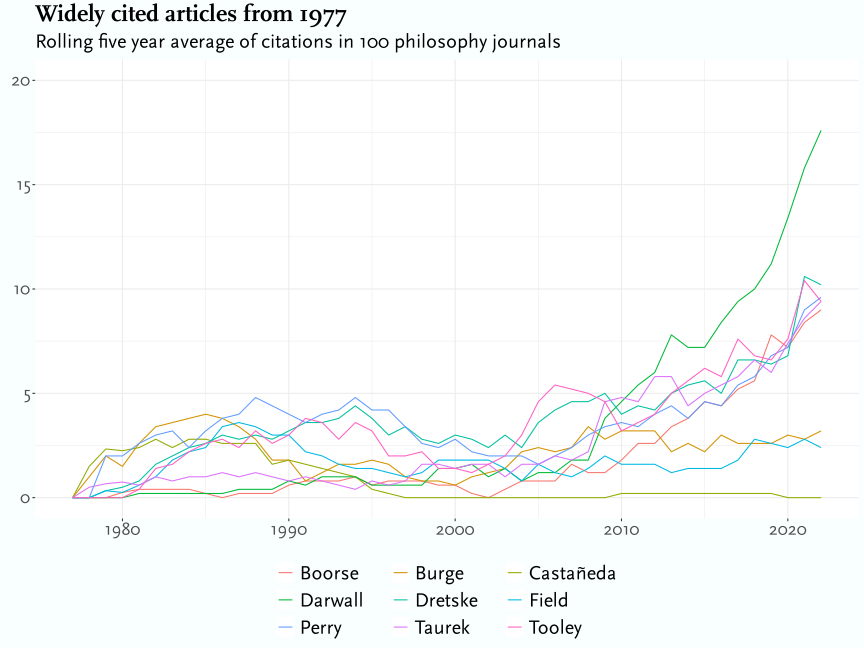
\includegraphics{citations_files/figure-pdf/fig-citation-spaghetti-1977-1.pdf}

}

\caption{\label{fig-citation-spaghetti-1977}Rolling five year average of
citation frequency for widely cited articles from 1977.}

\end{figure}%

\begin{figure}

\centering{

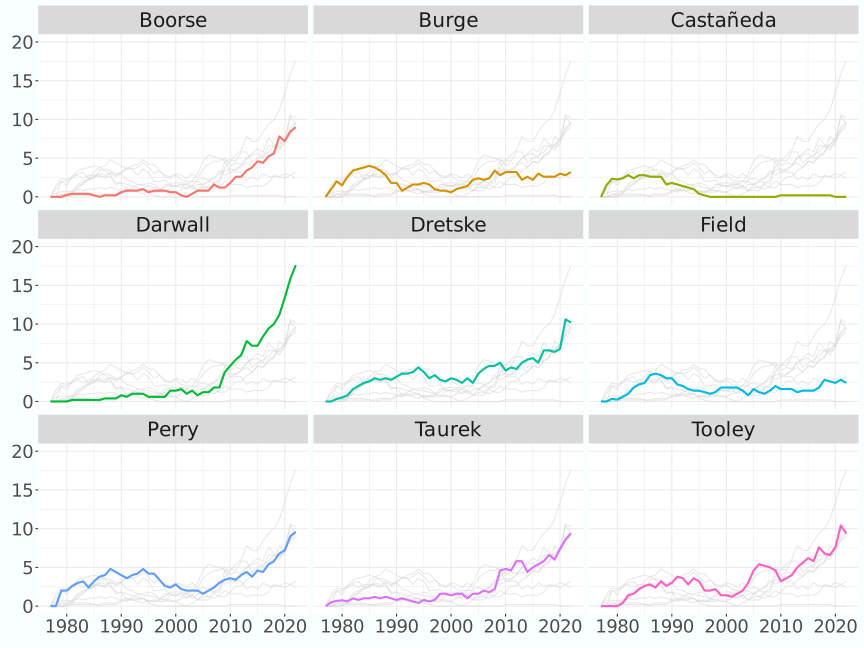
\includegraphics{citations_files/figure-pdf/fig-citation-facet-1977-1.pdf}

}

\caption{\label{fig-citation-facet-1977}Faceted version of
Figure~\ref{fig-citation-spaghetti-1977}.}

\end{figure}%

\newpage

\subsection{1978}\label{section-2}

\subsubsection*{Widely Cited Articles}\label{widely-cited-articles-2}
\addcontentsline{toc}{subsubsection}{Widely Cited Articles}

\begin{enumerate}
\def\labelenumi{\arabic{enumi}.}
\tightlist
\item
  D Lewis, ``Truth in Fiction'' \emph{American Philosophical Quarterly}
  15 (1): 37-46.
\item
  DL Hull, ``A Matter of Individuality'' \emph{Philosophy Of Science} 45
  (3): 335-360.
\item
  KL Walton, ``Fearing Fictions'' \emph{Journal Of Philosophy} 75 (1):
  5-27.
\item
  HG Frankfurt, ``The Problem of Action'' \emph{American Philosophical
  Quarterly} 15 (2): 157-162.
\item
  PR Thagard, ``The Best Explanation: Criteria for Theory Choice''
  \emph{Journal Of Philosophy} 75 (2): 76-92.
\item
  M Steiner, ``Mathematical Explanation'' \emph{Philosophical Studies}
  34 (2): 135-151.
\item
  J Kim, ``Supervenience and Nomological Incommensurables''
  \emph{American Philosophical Quarterly} 15 (2): 149-156.
\item
  GS Kavka, ``Some Paradoxes of Deterrence'' \emph{Journal Of
  Philosophy} 75 (6): 285-302.
\item
  L BonJour, ``Can Empirical Knowledge Have a Foundation?''
  \emph{American Philosophical Quarterly} 15 (1): 1-13.
\end{enumerate}

\subsubsection*{Citation Count}\label{citation-count-2}
\addcontentsline{toc}{subsubsection}{Citation Count}

\begin{longtable}[]{@{}lrrr@{}}

\caption{\label{tbl-citation-count-1978}Citation count for widely cited
articles from 1978.}

\tabularnewline

\toprule\noalign{}
Article & All & Early & Late \\
\midrule\noalign{}
\endhead
\bottomrule\noalign{}
\endlastfoot
Lewis & 167 & 19 & 100 \\
Hull & 145 & 17 & 55 \\
Walton & 97 & 22 & 43 \\
Frankfurt & 82 & 7 & 62 \\
Thagard & 80 & 10 & 47 \\
Kim & 76 & 34 & 2 \\
Steiner & 73 & 5 & 47 \\
BonJour & 51 & 17 & 14 \\
Kavka & 42 & 18 & 3 \\

\end{longtable}

\subsubsection*{Citation Rank}\label{citation-rank-2}
\addcontentsline{toc}{subsubsection}{Citation Rank}

\begin{longtable}[]{@{}lrrr@{}}

\caption{\label{tbl-citation-rank-1978}Citation rank for widely cited
articles from 1978.}

\tabularnewline

\toprule\noalign{}
Article & Overall & Early & Late \\
\midrule\noalign{}
\endhead
\bottomrule\noalign{}
\endlastfoot
Lewis & 1 & 3 & 1 \\
Hull & 2 & 5 & 3 \\
Walton & 3 & 2 & 6 \\
Frankfurt & 4 & 29 & 2 \\
Thagard & 5 & 17 & 4 \\
Kim & 6 & 1 & 92 \\
Steiner & 8 & 44 & 4 \\
BonJour & 14 & 5 & 16 \\
Kavka & 19 & 4 & 70 \\

\end{longtable}

\subsubsection*{Citation Trends}\label{citation-trends-2}
\addcontentsline{toc}{subsubsection}{Citation Trends}

\begin{figure}

\centering{

\includegraphics{citations_files/figure-pdf/fig-citation-spaghetti-1978-1.pdf}

}

\caption{\label{fig-citation-spaghetti-1978}Rolling five year average of
citation frequency for widely cited articles from 1978.}

\end{figure}%

\begin{figure}

\centering{

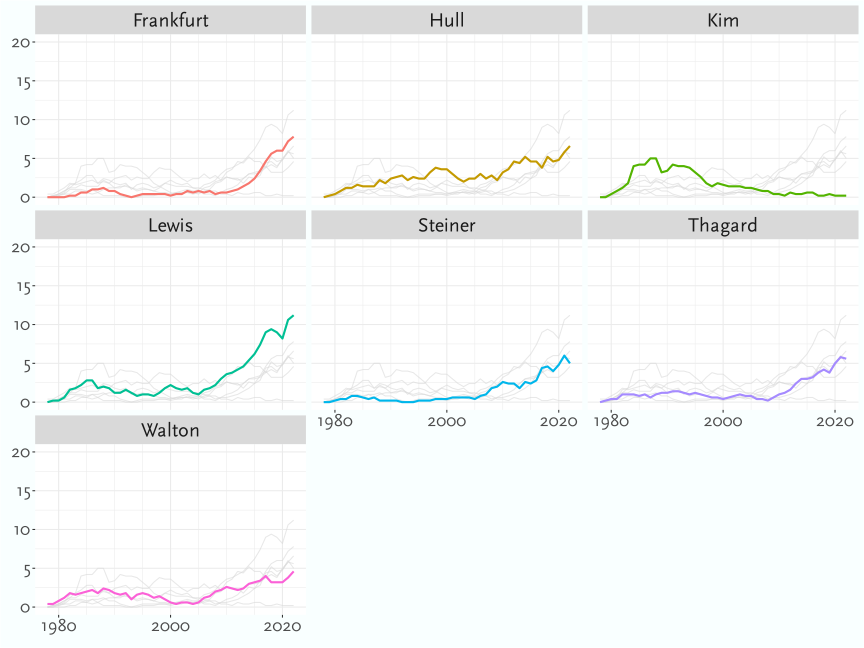
\includegraphics{citations_files/figure-pdf/fig-citation-facet-1978-1.pdf}

}

\caption{\label{fig-citation-facet-1978}Faceted version of
Figure~\ref{fig-citation-spaghetti-1978}.}

\end{figure}%

\newpage

\subsection{1979}\label{section-3}

\subsubsection*{Widely Cited Articles}\label{widely-cited-articles-3}
\addcontentsline{toc}{subsubsection}{Widely Cited Articles}

\begin{enumerate}
\def\labelenumi{\arabic{enumi}.}
\tightlist
\item
  J Perry, ``The Problem of the Essential Indexical'' \emph{Noûs} 13
  (1): 3-21.
\item
  D Lewis, ``Attitudes De Dicto and De Se'' \emph{Philosophical Review}
  88 (4): 513-543.
\item
  D Lewis, ``Counterfactual Dependence and Time's Arrow'' \emph{Noûs} 13
  (4): 455-476.
\item
  D Lewis, ``Scorekeeping in a Language Game'' \emph{Journal Of
  Philosophical Logic} 8 (3): 339-359.
\item
  J McDowell, ``Virtue and Reason'' \emph{Monist} 62 (3): 331-350.
\item
  G Priest, ``The Logic of Paradox'' \emph{Journal Of Philosophical
  Logic} 8 (2): 219-241.
\item
  N Daniels, ``Wide Reflective Equilibrium and Theory Acceptance in
  Ethics'' \emph{Journal Of Philosophy} 76 (5): 256-282.
\item
  N Cartwright, ``Causal Laws and Effective Strategies'' \emph{Noûs} 13
  (4): 419-437.
\item
  RM Adams, ``Primitive Thisness and Primitive Identity'' \emph{Journal
  Of Philosophy} 76 (1): 5-26.
\end{enumerate}

\subsubsection*{Citation Count}\label{citation-count-3}
\addcontentsline{toc}{subsubsection}{Citation Count}

\begin{longtable}[]{@{}lrrr@{}}

\caption{\label{tbl-citation-count-1979}Citation count for widely cited
articles from 1979.}

\tabularnewline

\toprule\noalign{}
Article & All & Early & Late \\
\midrule\noalign{}
\endhead
\bottomrule\noalign{}
\endlastfoot
Perry & 397 & 61 & 178 \\
Lewis, De Se & 383 & 37 & 229 \\
Lewis, Time's Arrow & 365 & 37 & 192 \\
Lewis, Scorekeeping & 359 & 15 & 206 \\
McDowell & 215 & 12 & 90 \\
Priest & 211 & 16 & 146 \\
Daniels & 143 & 40 & 53 \\
Adams & 133 & 25 & 63 \\
Cartwright & 129 & 29 & 50 \\

\end{longtable}

\subsubsection*{Citation Rank}\label{citation-rank-3}
\addcontentsline{toc}{subsubsection}{Citation Rank}

\begin{longtable}[]{@{}lrrr@{}}

\caption{\label{tbl-citation-rank-1979}Citation rank for widely cited
articles from 1979.}

\tabularnewline

\toprule\noalign{}
Article & Overall & Early & Late \\
\midrule\noalign{}
\endhead
\bottomrule\noalign{}
\endlastfoot
Perry & 1 & 1 & 4 \\
Lewis, De Se & 2 & 3 & 1 \\
Lewis, Time's Arrow & 3 & 3 & 3 \\
Lewis, Scorekeeping & 4 & 12 & 2 \\
McDowell & 5 & 16 & 6 \\
Priest & 6 & 10 & 5 \\
Daniels & 7 & 2 & 9 \\
Adams & 8 & 6 & 8 \\
Cartwright & 9 & 5 & 10 \\

\end{longtable}

\subsubsection*{Citation Trends}\label{citation-trends-3}
\addcontentsline{toc}{subsubsection}{Citation Trends}

\begin{figure}

\centering{

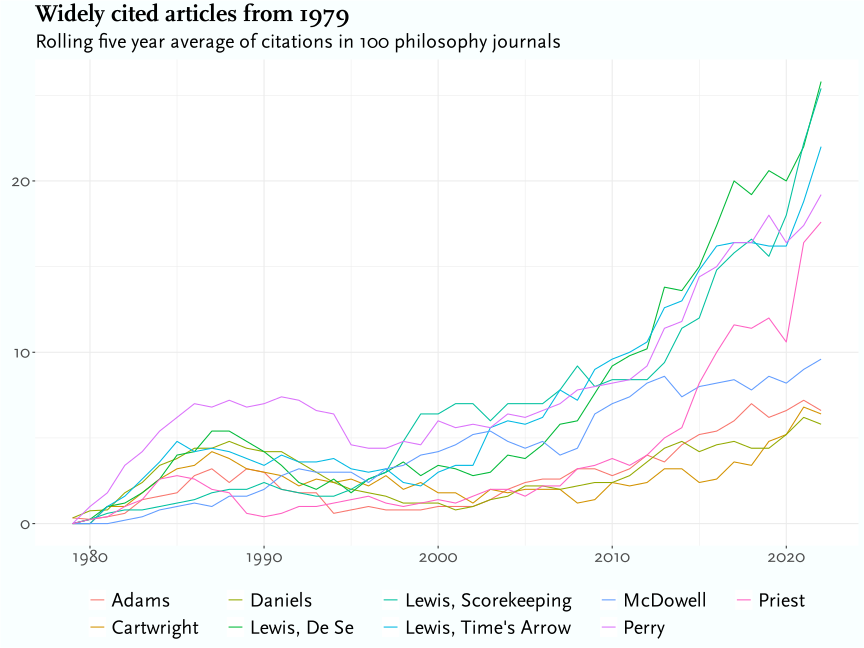
\includegraphics{citations_files/figure-pdf/fig-citation-spaghetti-1979-1.pdf}

}

\caption{\label{fig-citation-spaghetti-1979}Rolling five year average of
citation frequency for widely cited articles from 1979.}

\end{figure}%

\begin{figure}

\centering{

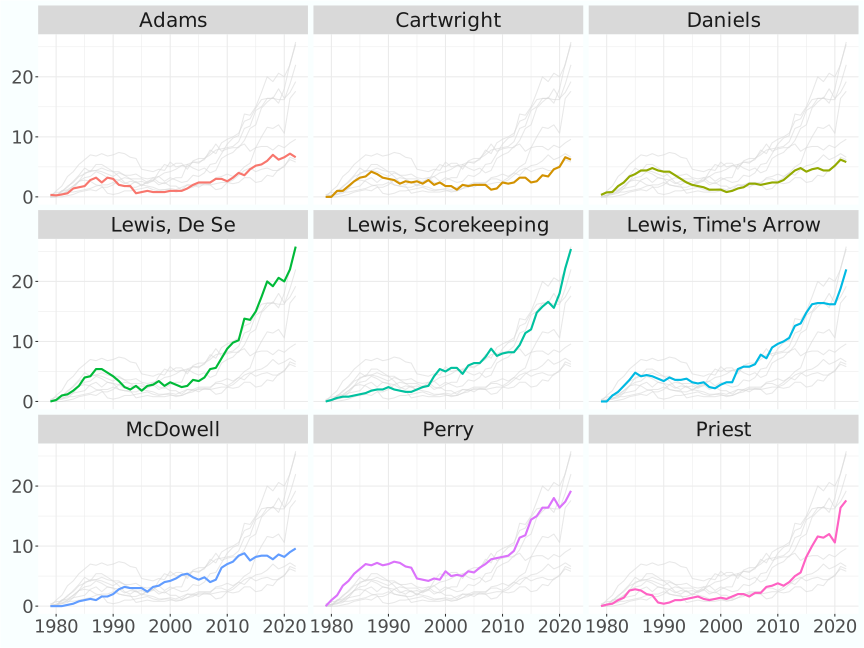
\includegraphics{citations_files/figure-pdf/fig-citation-facet-1979-1.pdf}

}

\caption{\label{fig-citation-facet-1979}Faceted version of
Figure~\ref{fig-citation-spaghetti-1979}.}

\end{figure}%

\newpage

\subsection{1980}\label{section-4}

\subsubsection*{Widely Cited Articles}\label{widely-cited-articles-4}
\addcontentsline{toc}{subsubsection}{Widely Cited Articles}

\begin{enumerate}
\def\labelenumi{\arabic{enumi}.}
\tightlist
\item
  J Rawls, ``Rational and Full Autonomy'' \emph{Journal Of Philosophy}
  77 (9): 515-535.
\item
  M Davies and L Humberstone, ``Two Notions of Necessity''
  \emph{Philosophical Studies} 38 (1): 1-30.
\item
  J Levinson, ``What a Musical Work Is'' \emph{Journal Of Philosophy} 77
  (1): 5-28.
\item
  E Sober, ``Evolution, Population Thinking, and Essentialism''
  \emph{Philosophy Of Science} 47 (3): 350-383.
\item
  D Lewis, ``Veridical Hallucination and Prosthetic Vision''
  \emph{Australasian Journal Of Philosophy} 58 (3): 239-249.
\item
  RB Marcus, ``Moral Dilemmas and Consistency'' \emph{Journal Of
  Philosophy} 77 (3): 121-136.
\item
  N Daniels, ``Reflective Equilibrium and Archimedean Points''
  \emph{Canadian Journal Of Philosophy} 10 (1): 83-103.
\item
  PS Churchland, ``A Perspective on Mind-Brain Research'' \emph{Journal
  Of Philosophy} 77 (4): 185-207.
\item
  N Block, ``Are Absent Qualia Impossible'' \emph{Philosophical Review}
  89 (2): 257-274.
\end{enumerate}

\subsubsection*{Citation Count}\label{citation-count-4}
\addcontentsline{toc}{subsubsection}{Citation Count}

\begin{longtable}[]{@{}lrrr@{}}

\caption{\label{tbl-citation-count-1980}Citation count for widely cited
articles from 1980.}

\tabularnewline

\toprule\noalign{}
Article & All & Early & Late \\
\midrule\noalign{}
\endhead
\bottomrule\noalign{}
\endlastfoot
Rawls & 188 & 52 & 58 \\
Davies and Humberstone & 125 & 3 & 61 \\
Levinson & 100 & 10 & 55 \\
Sober & 93 & 9 & 44 \\
Marcus & 82 & 24 & 35 \\
Lewis & 81 & 10 & 45 \\
Daniels & 41 & 22 & 8 \\
Block & 38 & 19 & 4 \\
Churchland & 23 & 19 & 0 \\

\end{longtable}

\subsubsection*{Citation Rank}\label{citation-rank-4}
\addcontentsline{toc}{subsubsection}{Citation Rank}

\begin{longtable}[]{@{}lrrr@{}}

\caption{\label{tbl-citation-rank-1980}Citation rank for widely cited
articles from 1980.}

\tabularnewline

\toprule\noalign{}
Article & Overall & Early & Late \\
\midrule\noalign{}
\endhead
\bottomrule\noalign{}
\endlastfoot
Rawls & 1 & 1 & 2 \\
Davies and Humberstone & 2 & 94 & 1 \\
Levinson & 3 & 10 & 3 \\
Sober & 4 & 14 & 5 \\
Marcus & 5 & 2 & 6 \\
Lewis & 6 & 10 & 4 \\
Daniels & 8 & 3 & 29 \\
Block & 11 & 4 & 67 \\
Churchland & 29 & 4 & 321 \\

\end{longtable}

\subsubsection*{Citation Trends}\label{citation-trends-4}
\addcontentsline{toc}{subsubsection}{Citation Trends}

\begin{figure}

\centering{

\includegraphics{citations_files/figure-pdf/fig-citation-spaghetti-1980-1.pdf}

}

\caption{\label{fig-citation-spaghetti-1980}Rolling five year average of
citation frequency for widely cited articles from 1980.}

\end{figure}%

\begin{figure}

\centering{

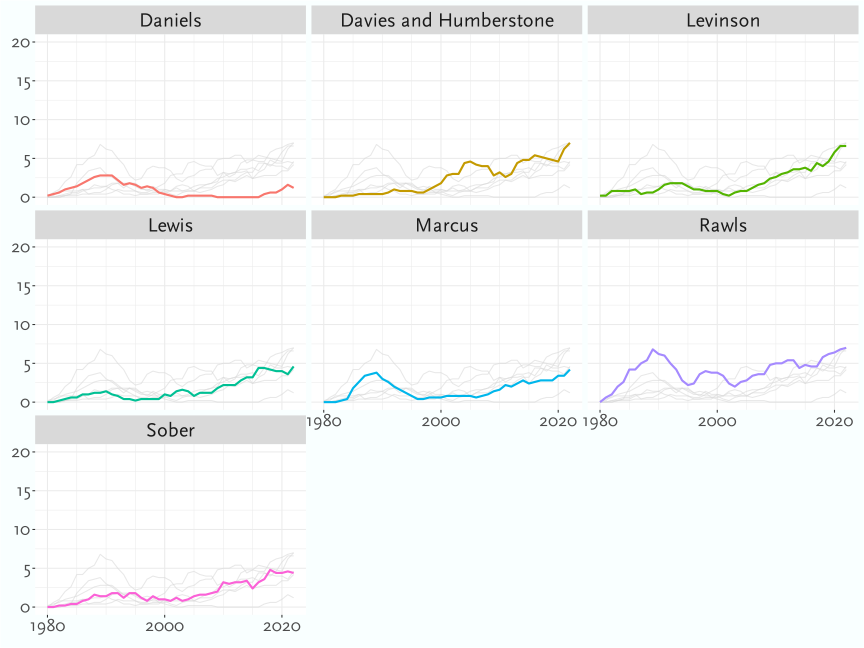
\includegraphics{citations_files/figure-pdf/fig-citation-facet-1980-1.pdf}

}

\caption{\label{fig-citation-facet-1980}Faceted version of
Figure~\ref{fig-citation-spaghetti-1980}.}

\end{figure}%

\newpage

\subsection{1981}\label{section-5}

\subsubsection*{Widely Cited Articles}\label{widely-cited-articles-5}
\addcontentsline{toc}{subsubsection}{Widely Cited Articles}

\begin{enumerate}
\def\labelenumi{\arabic{enumi}.}
\tightlist
\item
  L Laudan, ``A Confutation of Convergent Realism'' \emph{Philosophy Of
  Science} 48 (1): 19-49.
\item
  P Kitcher, ``Explanatory Unification'' \emph{Philosophy Of Science} 48
  (4): 507-531.
\item
  PM Churchland, ``Eliminative Materialism and the Propositional
  Attitudes'' \emph{Journal Of Philosophy} 78 (2): 67-90.
\item
  R Dworkin, ``What is Equality? Part 2: Equality of Resources''
  \emph{Philosophy \& Public Affairs} 10 (4): 283-345.
\item
  D Lewis, ``Causal Decision Theory'' \emph{Australasian Journal Of
  Philosophy} 59 (1): 5-30.
\item
  P van Inwagen, ``The Doctrine of Arbitrary Undetached Parts''
  \emph{Pacific Philosophical Quarterly} 62 (2): 123-137.
\item
  RM Adams, ``Actualism and Thisness'' \emph{Synthese} 49 (1): 3-41.
\item
  J Dupre, ``Natural Kinds and Biological Taxa'' \emph{Philosophical
  Review} 90 (1): 66-90.
\item
  R Dworkin, ``What is Equality? Part 1: Equality of Welfare''
  \emph{Philosophy \& Public Affairs} 10 (3): 185-246.
\end{enumerate}

\subsubsection*{Citation Count}\label{citation-count-5}
\addcontentsline{toc}{subsubsection}{Citation Count}

\begin{longtable}[]{@{}lrrr@{}}

\caption{\label{tbl-citation-count-1981}Citation count for widely cited
articles from 1981.}

\tabularnewline

\toprule\noalign{}
Article & All & Early & Late \\
\midrule\noalign{}
\endhead
\bottomrule\noalign{}
\endlastfoot
Laudan & 266 & 28 & 134 \\
Kitcher & 240 & 10 & 135 \\
Churchland & 239 & 58 & 107 \\
Dworkin Pt. 2 & 174 & 22 & 68 \\
Lewis & 161 & 32 & 96 \\
van Inwagen & 107 & 6 & 35 \\
Dupre & 90 & 16 & 26 \\
Adams & 88 & 13 & 48 \\
Dworkin Pt. 1 & 77 & 16 & 22 \\

\end{longtable}

\subsubsection*{Citation Rank}\label{citation-rank-5}
\addcontentsline{toc}{subsubsection}{Citation Rank}

\begin{longtable}[]{@{}lrrr@{}}

\caption{\label{tbl-citation-rank-1981}Citation rank for widely cited
articles from 1981.}

\tabularnewline

\toprule\noalign{}
Article & Overall & Early & Late \\
\midrule\noalign{}
\endhead
\bottomrule\noalign{}
\endlastfoot
Laudan & 1 & 3 & 2 \\
Kitcher & 2 & 14 & 1 \\
Churchland & 3 & 1 & 3 \\
Dworkin Pt. 2 & 4 & 4 & 5 \\
Lewis & 5 & 2 & 4 \\
van Inwagen & 6 & 39 & 9 \\
Dupre & 8 & 5 & 13 \\
Adams & 9 & 9 & 6 \\
Dworkin Pt. 1 & 11 & 5 & 20 \\

\end{longtable}

\subsubsection*{Citation Trends}\label{citation-trends-5}
\addcontentsline{toc}{subsubsection}{Citation Trends}

\begin{figure}

\centering{

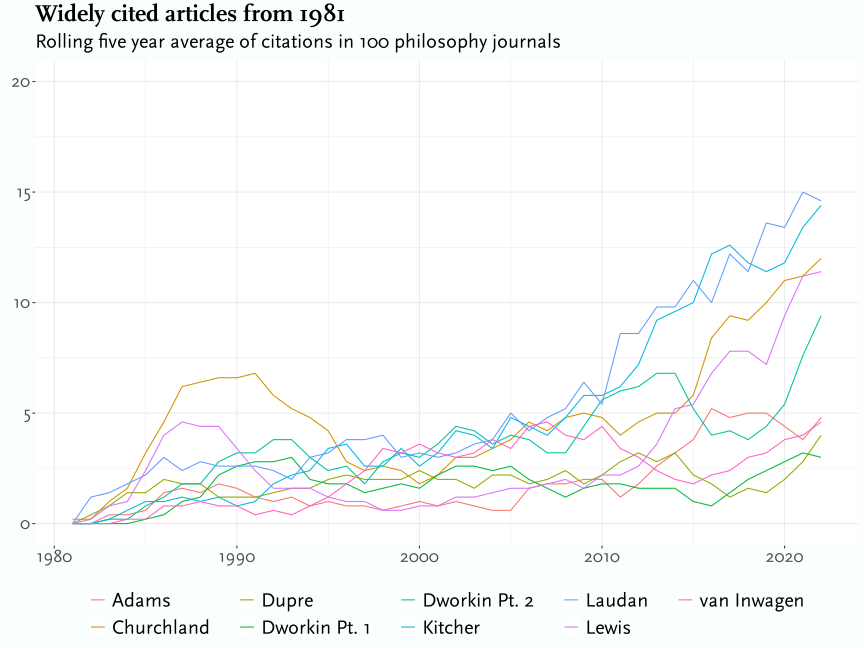
\includegraphics{citations_files/figure-pdf/fig-citation-spaghetti-1981-1.pdf}

}

\caption{\label{fig-citation-spaghetti-1981}Rolling five year average of
citation frequency for widely cited articles from 1981.}

\end{figure}%

\begin{figure}

\centering{

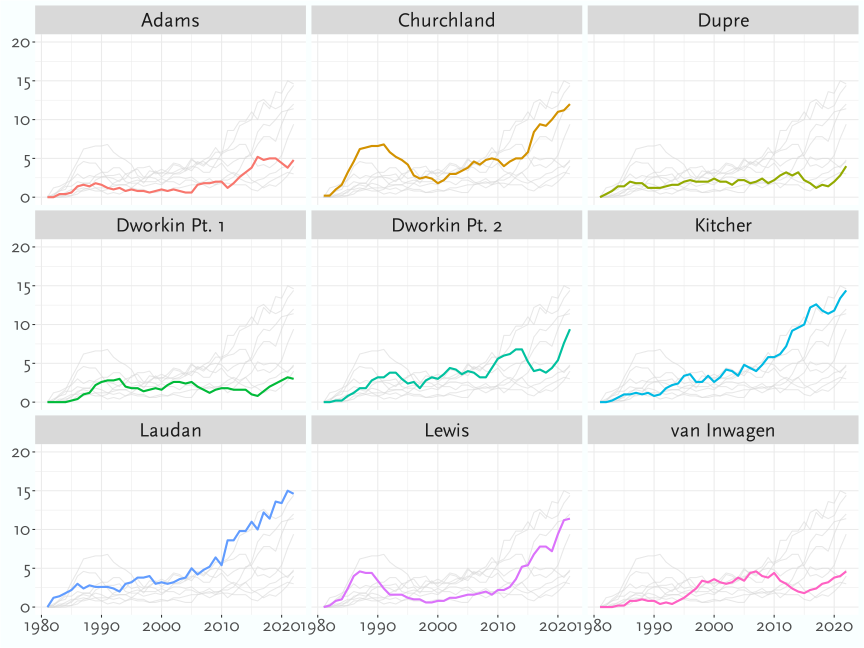
\includegraphics{citations_files/figure-pdf/fig-citation-facet-1981-1.pdf}

}

\caption{\label{fig-citation-facet-1981}Faceted version of
Figure~\ref{fig-citation-spaghetti-1981}.}

\end{figure}%

\newpage

\subsection{1982}\label{section-6}

\subsubsection*{Widely Cited Articles}\label{widely-cited-articles-6}
\addcontentsline{toc}{subsubsection}{Widely Cited Articles}

\begin{enumerate}
\def\labelenumi{\arabic{enumi}.}
\tightlist
\item
  F Jackson, ``Epiphenomenal Qualia'' \emph{Philosophical Quarterly} 32
  (127): 127-136.
\item
  S Wolf, ``Moral Saints'' \emph{Journal Of Philosophy} 79 (8): 419-439.
\item
  EW Prior, et al, ``Three Theses About Dispositions'' \emph{American
  Philosophical Quarterly} 19 (3): 251-257.
\item
  C Swoyer, ``The Nature of Natural Laws'' \emph{Australasian Journal Of
  Philosophy} 60 (3): 203-223.
\item
  D Lewis, ``Logic for Equivocators'' \emph{Noûs} 16 (3): 431-441.
\item
  J Haugeland, ``Weak Supervenience'' \emph{American Philosophical
  Quarterly} 19 (1): 93-103.
\item
  J Kim, ``Psychophysical Supervenience'' \emph{Philosophical Studies}
  41 (1): 51-70.
\item
  A Gupta, ``Truth and Paradox'' \emph{Journal Of Philosophical Logic}
  11 (1): 1-60.
\item
  D Shapere, ``The Concept of Observation in Science and Philosophy''
  \emph{Philosophy Of Science} 49 (4): 485-525.
\end{enumerate}

\subsubsection*{Citation Count}\label{citation-count-6}
\addcontentsline{toc}{subsubsection}{Citation Count}

\begin{longtable}[]{@{}lrrr@{}}

\caption{\label{tbl-citation-count-1982}Citation count for widely cited
articles from 1982.}

\tabularnewline

\toprule\noalign{}
Article & All & Early & Late \\
\midrule\noalign{}
\endhead
\bottomrule\noalign{}
\endlastfoot
Jackson & 455 & 26 & 227 \\
Wolf & 152 & 17 & 68 \\
Prior et al & 129 & 10 & 62 \\
Swoyer & 110 & 9 & 46 \\
Lewis & 87 & 3 & 73 \\
Gupta & 85 & 23 & 39 \\
Kim & 81 & 23 & 17 \\
Shapere & 47 & 21 & 10 \\
Haugeland & 44 & 26 & 3 \\

\end{longtable}

\subsubsection*{Citation Rank}\label{citation-rank-6}
\addcontentsline{toc}{subsubsection}{Citation Rank}

\begin{longtable}[]{@{}lrrr@{}}

\caption{\label{tbl-citation-rank-1982}Citation rank for widely cited
articles from 1982.}

\tabularnewline

\toprule\noalign{}
Article & Overall & Early & Late \\
\midrule\noalign{}
\endhead
\bottomrule\noalign{}
\endlastfoot
Jackson & 1 & 1 & 1 \\
Wolf & 2 & 7 & 3 \\
Prior et al & 3 & 19 & 4 \\
Swoyer & 4 & 24 & 5 \\
Lewis & 5 & 111 & 2 \\
Gupta & 6 & 3 & 7 \\
Kim & 7 & 3 & 18 \\
Shapere & 15 & 5 & 36 \\
Haugeland & 19 & 1 & 115 \\

\end{longtable}

\subsubsection*{Citation Trends}\label{citation-trends-6}
\addcontentsline{toc}{subsubsection}{Citation Trends}

\begin{figure}

\centering{

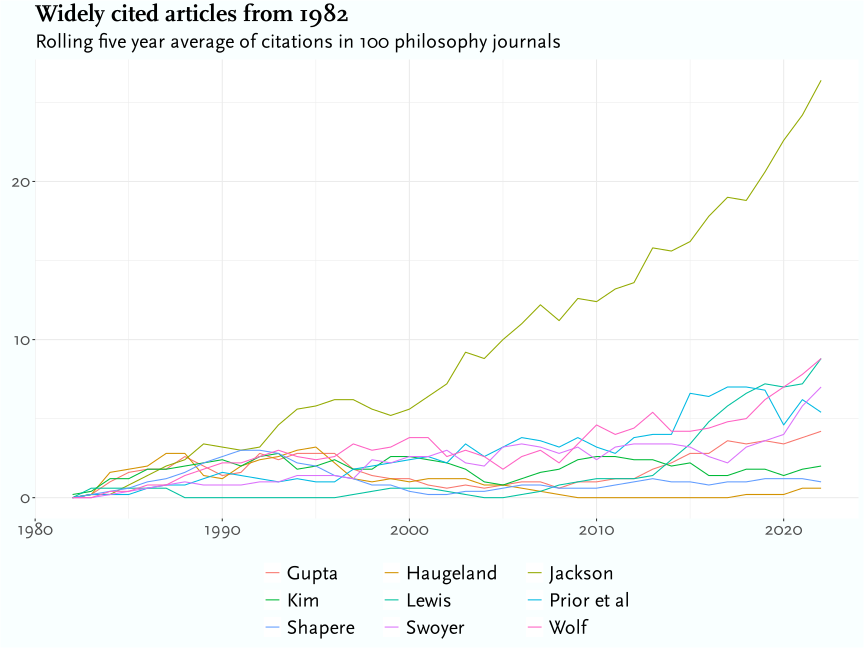
\includegraphics{citations_files/figure-pdf/fig-citation-spaghetti-1982-1.pdf}

}

\caption{\label{fig-citation-spaghetti-1982}Rolling five year average of
citation frequency for widely cited articles from 1982.}

\end{figure}%

\begin{figure}

\centering{

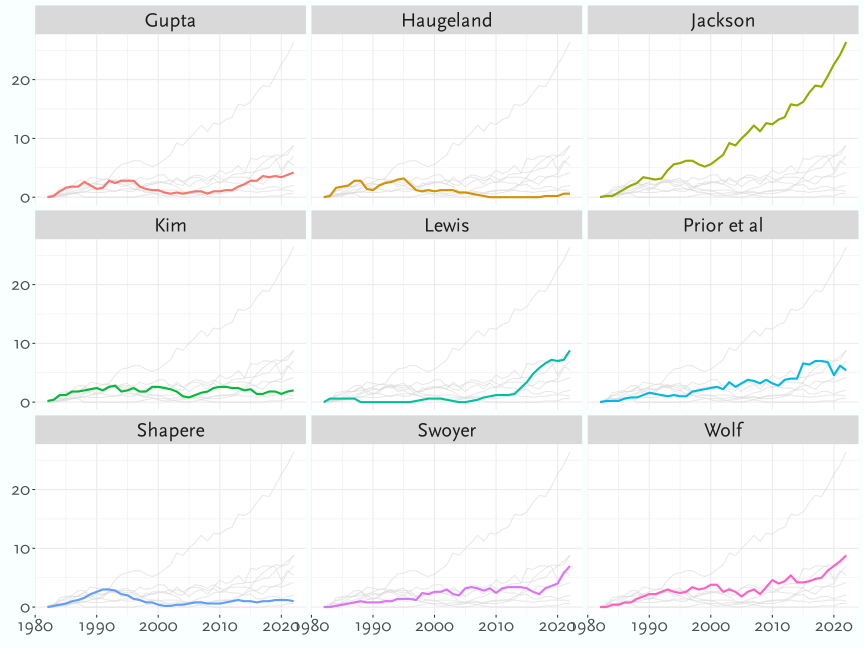
\includegraphics{citations_files/figure-pdf/fig-citation-facet-1982-1.pdf}

}

\caption{\label{fig-citation-facet-1982}Faceted version of
Figure~\ref{fig-citation-spaghetti-1982}.}

\end{figure}%

\newpage

\subsection{1983}\label{section-7}

\subsubsection*{Widely Cited Articles}\label{widely-cited-articles-7}
\addcontentsline{toc}{subsubsection}{Widely Cited Articles}

\begin{enumerate}
\def\labelenumi{\arabic{enumi}.}
\tightlist
\item
  D Lewis, ``New Work for a Theory of Universals'' \emph{Australasian
  Journal Of Philosophy} 61 (4): 343-377.
\item
  J Levine, ``Materialism and Qualia: The Explanatory Gap''
  \emph{Pacific Philosophical Quarterly} 64 (4): 354-361.
\item
  GS Kavka, ``The Toxin Puzzle'' \emph{Analysis} 43 (1): 33-36.
\item
  CM Korsgaard, ``Two Distinctions in Goodness'' \emph{Philosophical
  Review} 92 (2): 169-195.
\item
  R Brandom, ``Asserting'' \emph{Noûs} 17 (4): 637-650.
\item
  H Kornblith, ``Justified Belief and Epistemically Responsible Action''
  \emph{Philosophical Review} 92 (1): 33-48.
\item
  E Eells and E Sober, ``Probabilistic Causality and the Question of
  Transitivity'' \emph{Philosophy Of Science} 50 (1): 35-57.
\item
  PS Churchland and PM Churchland, ``Stalking The Wild Epistemic
  Engine'' \emph{Noûs} 17 (1): 5-18.
\item
  PS Churchland, ``Consciousness the Transmutation of a Concept''
  \emph{Pacific Philosophical Quarterly} 64 (1): 80-95.
\end{enumerate}

\subsubsection*{Citation Count}\label{citation-count-7}
\addcontentsline{toc}{subsubsection}{Citation Count}

\begin{longtable}[]{@{}lrrr@{}}

\caption{\label{tbl-citation-count-1983}Citation count for widely cited
articles from 1983.}

\tabularnewline

\toprule\noalign{}
Article & All & Early & Late \\
\midrule\noalign{}
\endhead
\bottomrule\noalign{}
\endlastfoot
Lewis & 767 & 46 & 515 \\
Levine & 212 & 2 & 107 \\
Kavka & 164 & 15 & 84 \\
Korsgaard & 135 & 5 & 88 \\
Brandom & 98 & 7 & 57 \\
Kornblith & 80 & 21 & 39 \\
Eells and Sober & 40 & 20 & 5 \\
Churchland and Churchland & 24 & 14 & 1 \\
Churchland & 23 & 14 & 4 \\

\end{longtable}

\subsubsection*{Citation Rank}\label{citation-rank-7}
\addcontentsline{toc}{subsubsection}{Citation Rank}

\begin{longtable}[]{@{}lrrr@{}}

\caption{\label{tbl-citation-rank-1983}Citation rank for widely cited
articles from 1983.}

\tabularnewline

\toprule\noalign{}
Article & Overall & Early & Late \\
\midrule\noalign{}
\endhead
\bottomrule\noalign{}
\endlastfoot
Lewis & 1 & 1 & 1 \\
Levine & 2 & 177 & 2 \\
Kavka & 3 & 4 & 4 \\
Korsgaard & 4 & 49 & 3 \\
Brandom & 5 & 26 & 5 \\
Kornblith & 9 & 2 & 10 \\
Eells and Sober & 14 & 3 & 63 \\
Churchland and Churchland & 32 & 5 & 200 \\
Churchland & 35 & 5 & 78 \\

\end{longtable}

\subsubsection*{Citation Trends}\label{citation-trends-7}
\addcontentsline{toc}{subsubsection}{Citation Trends}

\begin{figure}

\centering{

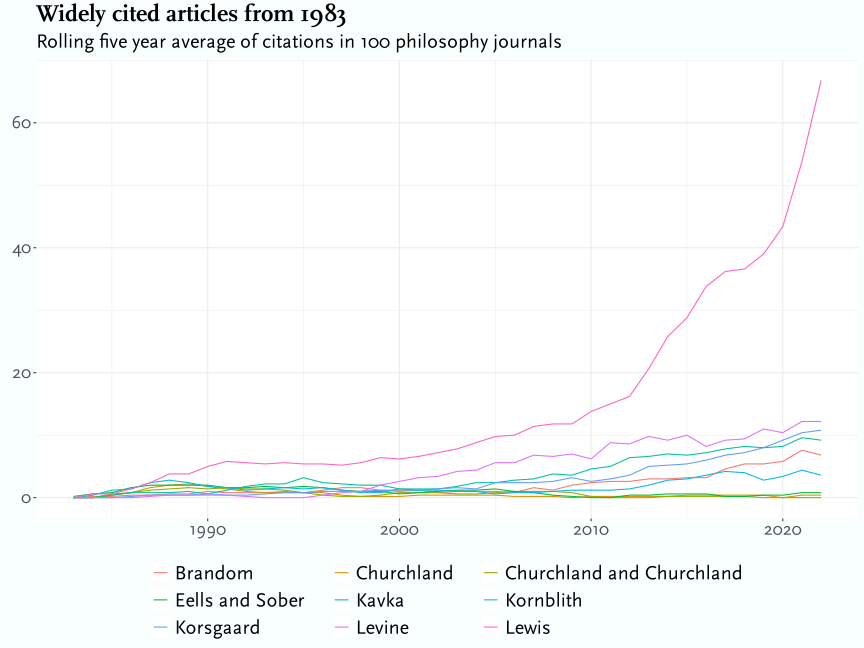
\includegraphics{citations_files/figure-pdf/fig-citation-spaghetti-1983-1.pdf}

}

\caption{\label{fig-citation-spaghetti-1983}Rolling five year average of
citation frequency for widely cited articles from 1983.}

\end{figure}%

\begin{figure}

\centering{

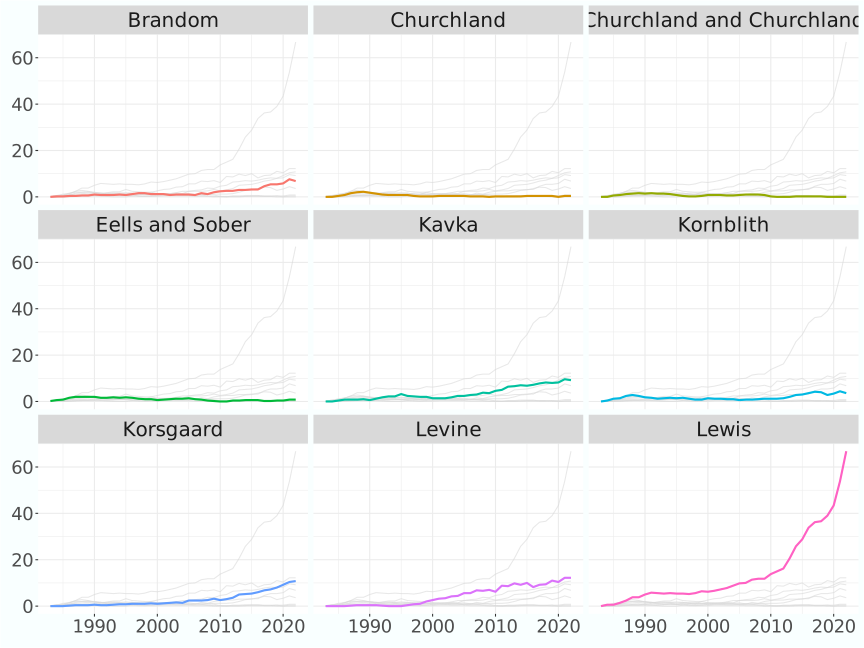
\includegraphics{citations_files/figure-pdf/fig-citation-facet-1983-1.pdf}

}

\caption{\label{fig-citation-facet-1983}Faceted version of
Figure~\ref{fig-citation-spaghetti-1983}.}

\end{figure}%

\newpage

\subsection{1984}\label{section-8}

\subsubsection*{Widely Cited Articles}\label{widely-cited-articles-8}
\addcontentsline{toc}{subsubsection}{Widely Cited Articles}

\begin{enumerate}
\def\labelenumi{\arabic{enumi}.}
\tightlist
\item
  D Lewis, ``Putnam's Paradox'' \emph{Australasian Journal Of
  Philosophy} 62 (3): 221-236.
\item
  BC van Fraassen, ``Belief and the Will'' \emph{Journal Of Philosophy}
  81 (5): 235-256.
\item
  P Railton, ``Alienation, Consequentialism, and the Demands of
  Morality'' \emph{Philosophy \& Public Affairs} 13 (2): 134-171.
\item
  G Boolos, ``To Be is To Be a Value of a Variable (Or To Be Some Values
  of Some Variables)'' \emph{Journal Of Philosophy} 81 (8): 430-449.
\item
  J Kim, ``Concepts of Supervenience'' \emph{Philosophy And
  Phenomenological Research} 45 (2): 153-176.
\item
  S Cohen, ``Justification and Truth'' \emph{Philosophical Studies} 46
  (3): 279-295.
\item
  J Fodor, ``Observation Reconsidered'' \emph{Philosophy Of Science} 51
  (1): 23-43.
\item
  J Kim, ``Epiphenomenal and Supervenient Causation'' \emph{Midwest
  Studies In Philosophy} 9: 257-270.
\item
  P Kitcher, ``Species'' \emph{Philosophy Of Science} 51 (2): 308-333.
\end{enumerate}

\subsubsection*{Citation Count}\label{citation-count-8}
\addcontentsline{toc}{subsubsection}{Citation Count}

\begin{longtable}[]{@{}lrrr@{}}

\caption{\label{tbl-citation-count-1984}Citation count for widely cited
articles from 1984.}

\tabularnewline

\toprule\noalign{}
Article & All & Early & Late \\
\midrule\noalign{}
\endhead
\bottomrule\noalign{}
\endlastfoot
Lewis & 235 & 20 & 129 \\
Fraassen & 208 & 19 & 101 \\
Railton & 198 & 19 & 112 \\
Boolos & 186 & 12 & 104 \\
Kim, Concepts & 157 & 50 & 35 \\
Cohen & 152 & 10 & 100 \\
Kitcher & 116 & 20 & 47 \\
Fodor & 83 & 21 & 34 \\
Kim, Epiphenomenal & 61 & 20 & 10 \\

\end{longtable}

\subsubsection*{Citation Rank}\label{citation-rank-8}
\addcontentsline{toc}{subsubsection}{Citation Rank}

\begin{longtable}[]{@{}lrrr@{}}

\caption{\label{tbl-citation-rank-1984}Citation rank for widely cited
articles from 1984.}

\tabularnewline

\toprule\noalign{}
Article & Overall & Early & Late \\
\midrule\noalign{}
\endhead
\bottomrule\noalign{}
\endlastfoot
Lewis & 1 & 3 & 1 \\
Fraassen & 2 & 6 & 4 \\
Railton & 3 & 6 & 2 \\
Boolos & 4 & 14 & 3 \\
Kim, Concepts & 5 & 1 & 10 \\
Cohen & 6 & 20 & 5 \\
Kitcher & 7 & 3 & 7 \\
Fodor & 10 & 2 & 11 \\
Kim, Epiphenomenal & 13 & 3 & 47 \\

\end{longtable}

\subsubsection*{Citation Trends}\label{citation-trends-8}
\addcontentsline{toc}{subsubsection}{Citation Trends}

\begin{figure}

\centering{

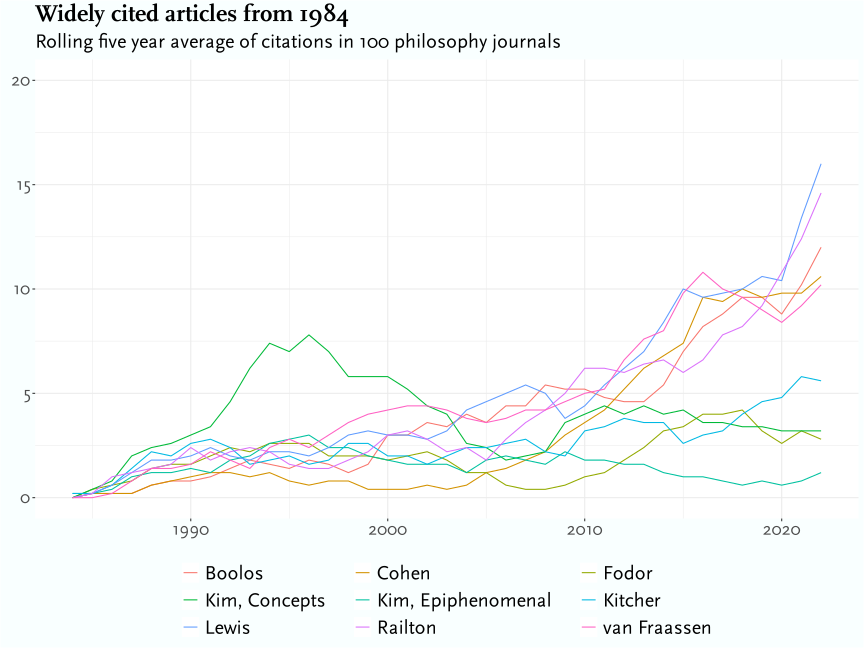
\includegraphics{citations_files/figure-pdf/fig-citation-spaghetti-1984-1.pdf}

}

\caption{\label{fig-citation-spaghetti-1984}Rolling five year average of
citation frequency for widely cited articles from 1984.}

\end{figure}%

\begin{figure}

\centering{

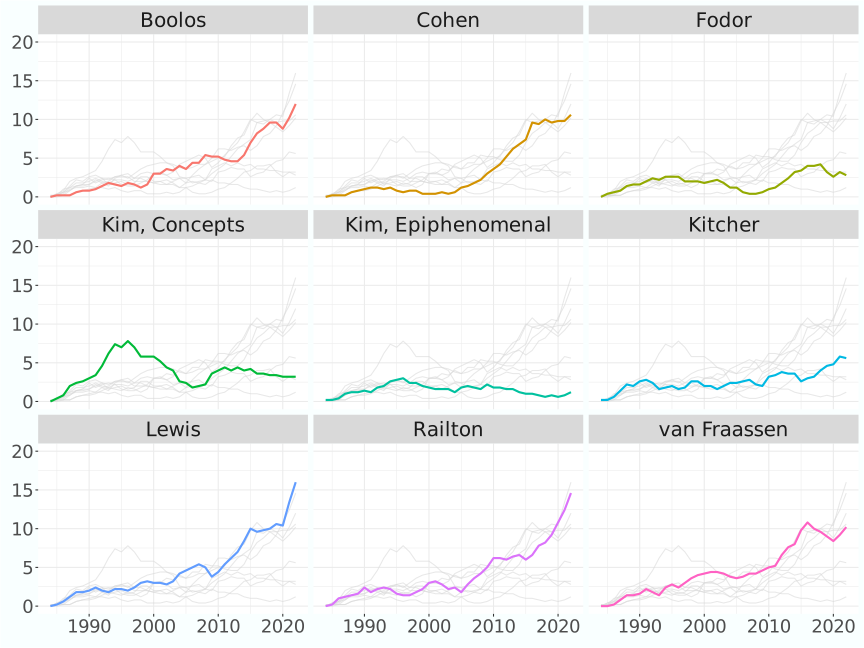
\includegraphics{citations_files/figure-pdf/fig-citation-facet-1984-1.pdf}

}

\caption{\label{fig-citation-facet-1984}Faceted version of
Figure~\ref{fig-citation-spaghetti-1984}.}

\end{figure}%

\newpage

\subsection{1985}\label{section-9}

\subsubsection*{Widely Cited Articles}\label{widely-cited-articles-9}
\addcontentsline{toc}{subsubsection}{Widely Cited Articles}

\begin{enumerate}
\def\labelenumi{\arabic{enumi}.}
\tightlist
\item
  R Feldman and E Conee, ``Evidentialism'' \emph{Philosophical Studies}
  48 (1): 15-34.
\item
  E McMullin, ``Galilean Idealization'' \emph{Studies In History And
  Philosophy Of Science} 16 (3): 247-273.
\item
  J Hardwig, ``Epistemic Dependence'' \emph{Journal Of Philosophy} 82
  (7): 335-349.
\item
  V McGee, ``A Counterexample To Modus-Ponens'' \emph{Journal Of
  Philosophy} 82 (9): 462-471.
\item
  G Boolos, ``Nominalist Platonism'' \emph{Philosophical Review} 94 (3):
  327-344.
\item
  RM Adams, ``Involuntary Sins'' \emph{Philosophical Review} 94 (1):
  3-31.
\item
  J Rawls, ``Justice as Fairness: Political Not Metaphysical''
  \emph{Philosophy \& Public Affairs} 14 (3): 223-251.
\item
  PM Churchland, ``Reduction, Qualia, and the Direct Introspection of
  Brain States'' \emph{Journal Of Philosophy} 82 (1): 8-28.
\item
  R Feldman, ``Reliability and Justification'' \emph{Monist} 68 (2):
  159-174.
\end{enumerate}

\subsubsection*{Citation Count}\label{citation-count-9}
\addcontentsline{toc}{subsubsection}{Citation Count}

\begin{longtable}[]{@{}lrrr@{}}

\caption{\label{tbl-citation-count-1985}Citation count for widely cited
articles from 1985.}

\tabularnewline

\toprule\noalign{}
Article & All & Early & Late \\
\midrule\noalign{}
\endhead
\bottomrule\noalign{}
\endlastfoot
Feldman and Conee & 174 & 6 & 118 \\
McMullin & 142 & 5 & 89 \\
Hardwig & 135 & 10 & 84 \\
McGee & 126 & 7 & 93 \\
Boolos & 97 & 9 & 42 \\
Rawls & 89 & 42 & 22 \\
Adams & 78 & 4 & 53 \\
Feldman & 76 & 19 & 28 \\
Churchland & 67 & 21 & 16 \\

\end{longtable}

\subsubsection*{Citation Rank}\label{citation-rank-9}
\addcontentsline{toc}{subsubsection}{Citation Rank}

\begin{longtable}[]{@{}lrrr@{}}

\caption{\label{tbl-citation-rank-1985}Citation rank for widely cited
articles from 1985.}

\tabularnewline

\toprule\noalign{}
Article & Overall & Early & Late \\
\midrule\noalign{}
\endhead
\bottomrule\noalign{}
\endlastfoot
Feldman and Conee & 1 & 30 & 1 \\
McMullin & 2 & 50 & 3 \\
Hardwig & 3 & 7 & 4 \\
McGee & 4 & 21 & 2 \\
Boolos & 5 & 10 & 6 \\
Rawls & 6 & 1 & 11 \\
Adams & 8 & 68 & 5 \\
Feldman & 9 & 3 & 9 \\
Churchland & 10 & 2 & 19 \\

\end{longtable}

\subsubsection*{Citation Trends}\label{citation-trends-9}
\addcontentsline{toc}{subsubsection}{Citation Trends}

\begin{figure}

\centering{

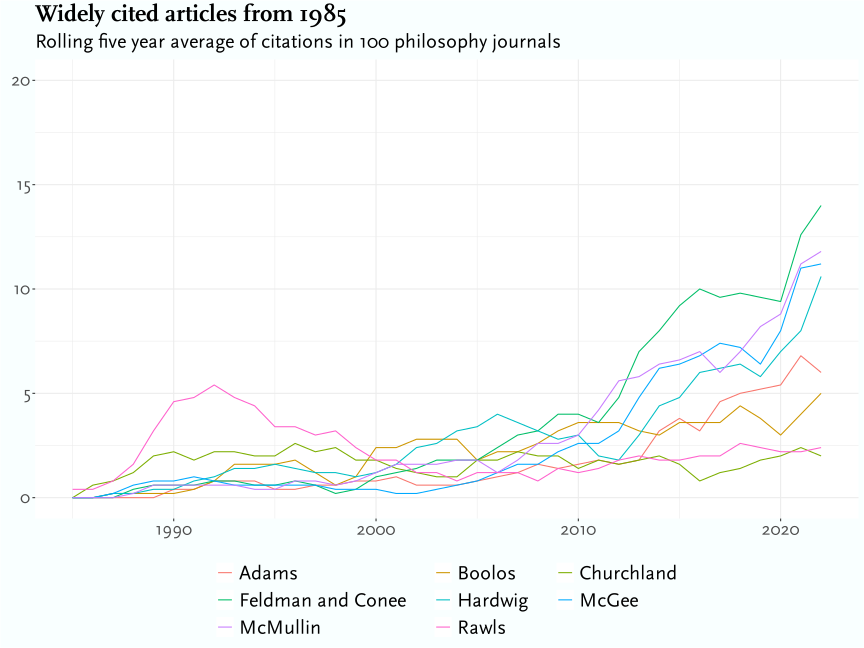
\includegraphics{citations_files/figure-pdf/fig-citation-spaghetti-1985-1.pdf}

}

\caption{\label{fig-citation-spaghetti-1985}Rolling five year average of
citation frequency for widely cited articles from 1985.}

\end{figure}%

\begin{figure}

\centering{

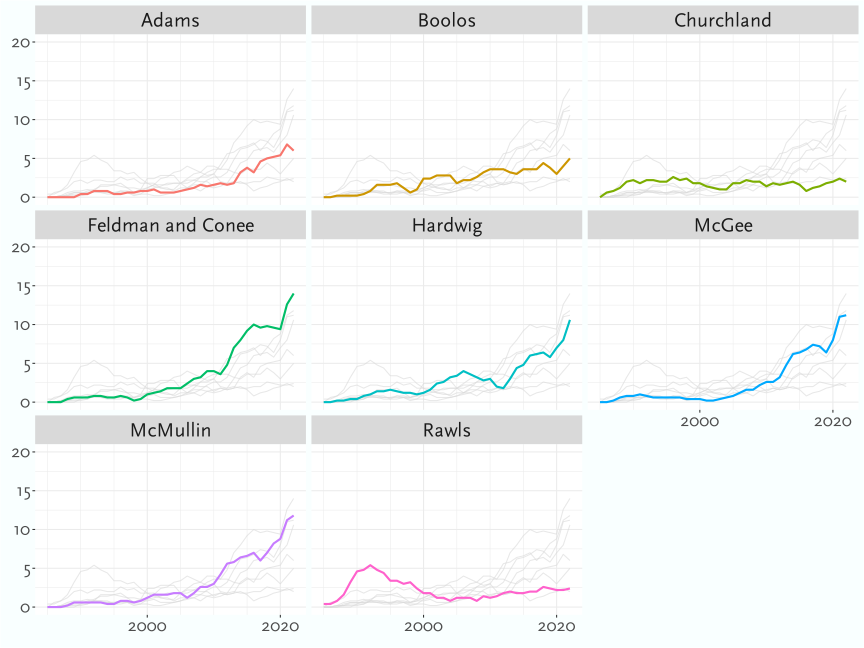
\includegraphics{citations_files/figure-pdf/fig-citation-facet-1985-1.pdf}

}

\caption{\label{fig-citation-facet-1985}Faceted version of
Figure~\ref{fig-citation-spaghetti-1985}.}

\end{figure}%

\newpage

\subsection{1986}\label{section-10}

\subsubsection*{Widely Cited Articles}\label{widely-cited-articles-10}
\addcontentsline{toc}{subsubsection}{Widely Cited Articles}

\begin{enumerate}
\def\labelenumi{\arabic{enumi}.}
\tightlist
\item
  P Railton, ``Moral Realism'' \emph{Philosophical Review} 95 (2):
  163-207.
\item
  T Burge, ``Individualism and Psychology'' \emph{Philosophical Review}
  95 (1): 3-45.
\item
  CM Korsgaard, ``Skepticism About Practical Reason'' \emph{Journal Of
  Philosophy} 83 (1): 5-25.
\item
  A Baier, ``Trust and Antitrust'' \emph{Ethics} 96 (2): 231-260.
\item
  DM Rosenthal, ``Two Concepts of Consciousness'' \emph{Philosophical
  Studies} 49 (3): 329-359.
\item
  F Jackson and R Pargetter, ``Oughts, Options, and Actualism''
  \emph{Philosophical Review} 95 (2): 233-255.
\item
  N Block, ``Advertisement for a Semantics for Psychology''
  \emph{Midwest Studies In Philosophy} 10: 615-678.
\item
  RG Millikan, ``Thoughts Without Laws, Cognitive Science With Content''
  \emph{Philosophical Review} 95 (1): 47-80.
\item
  AL Brueckner, ``Brains in a Vat'' \emph{Journal Of Philosophy} 83 (3):
  148-167.
\end{enumerate}

\subsubsection*{Citation Count}\label{citation-count-10}
\addcontentsline{toc}{subsubsection}{Citation Count}

\begin{longtable}[]{@{}lrrr@{}}

\caption{\label{tbl-citation-count-1986}Citation count for widely cited
articles from 1986.}

\tabularnewline

\toprule\noalign{}
Article & All & Early & Late \\
\midrule\noalign{}
\endhead
\bottomrule\noalign{}
\endlastfoot
Railton & 234 & 40 & 111 \\
Burge & 164 & 53 & 47 \\
Korsgaard & 151 & 15 & 70 \\
Baier & 138 & 23 & 87 \\
Rosenthal & 112 & 9 & 44 \\
Block & 109 & 18 & 49 \\
Jackson and Pargetter & 99 & 10 & 66 \\
Millikan & 39 & 22 & 3 \\
Brueckner & 33 & 18 & 6 \\

\end{longtable}

\subsubsection*{Citation Rank}\label{citation-rank-10}
\addcontentsline{toc}{subsubsection}{Citation Rank}

\begin{longtable}[]{@{}lrrr@{}}

\caption{\label{tbl-citation-rank-1986}Citation rank for widely cited
articles from 1986.}

\tabularnewline

\toprule\noalign{}
Article & Overall & Early & Late \\
\midrule\noalign{}
\endhead
\bottomrule\noalign{}
\endlastfoot
Railton & 1 & 2 & 1 \\
Burge & 2 & 1 & 6 \\
Korsgaard & 3 & 8 & 3 \\
Baier & 4 & 3 & 2 \\
Rosenthal & 5 & 25 & 8 \\
Block & 6 & 5 & 5 \\
Jackson and Pargetter & 8 & 17 & 4 \\
Millikan & 24 & 4 & 132 \\
Brueckner & 31 & 5 & 74 \\

\end{longtable}

\subsubsection*{Citation Trends}\label{citation-trends-10}
\addcontentsline{toc}{subsubsection}{Citation Trends}

\begin{figure}

\centering{

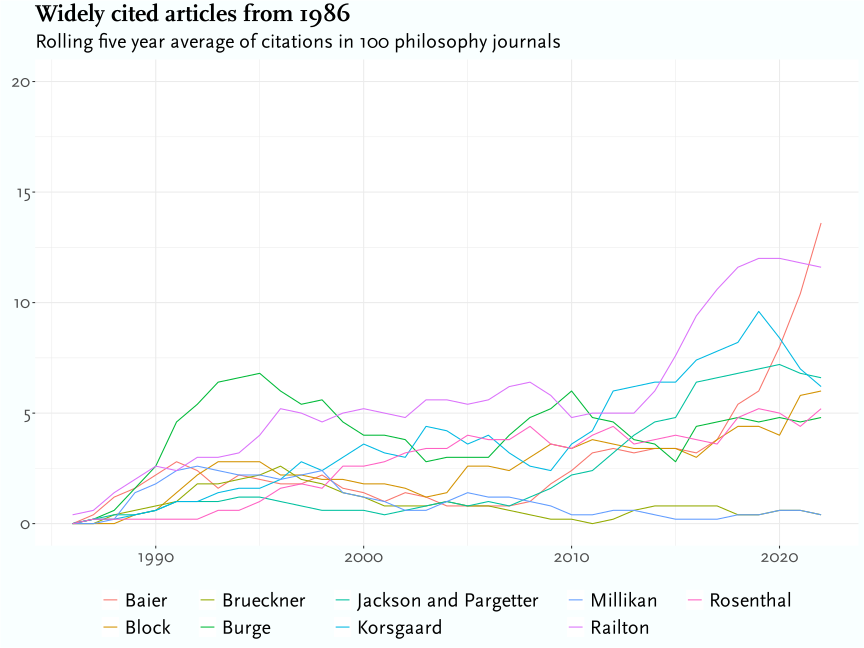
\includegraphics{citations_files/figure-pdf/fig-citation-spaghetti-1986-1.pdf}

}

\caption{\label{fig-citation-spaghetti-1986}Rolling five year average of
citation frequency for widely cited articles from 1986.}

\end{figure}%

\begin{figure}

\centering{

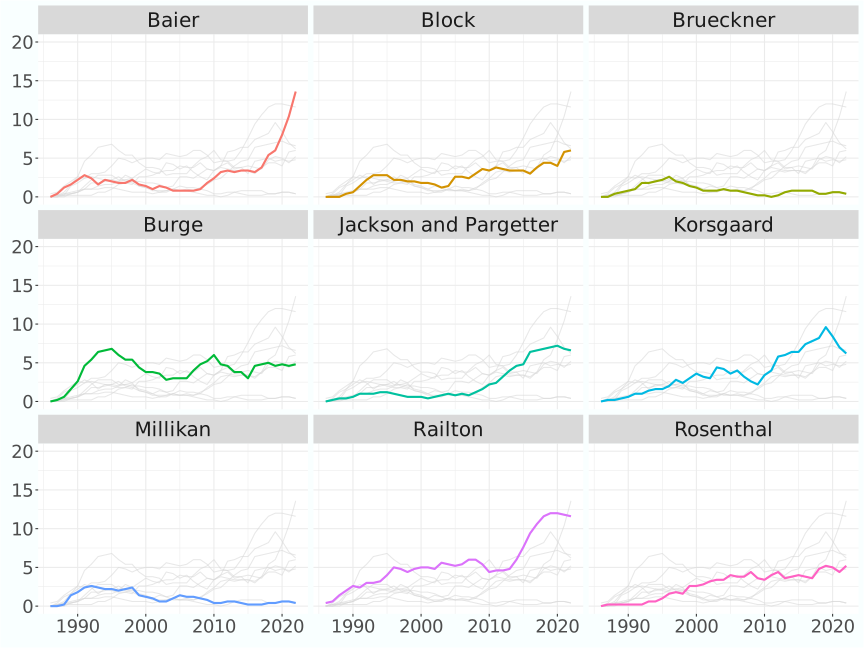
\includegraphics{citations_files/figure-pdf/fig-citation-facet-1986-1.pdf}

}

\caption{\label{fig-citation-facet-1986}Faceted version of
Figure~\ref{fig-citation-spaghetti-1986}.}

\end{figure}%

\newpage

\subsection{1987}\label{section-11}

\subsubsection*{Widely Cited Articles}\label{widely-cited-articles-11}
\addcontentsline{toc}{subsubsection}{Widely Cited Articles}

\begin{enumerate}
\def\labelenumi{\arabic{enumi}.}
\tightlist
\item
  M Smith, ``The Humean Theory of Motivation'' \emph{Mind} 96 (381):
  36-61.
\item
  J Bigelow and R Pargetter, ``Functions'' \emph{Journal Of Philosophy}
  84 (4): 181-196.
\item
  H Frankfurt, ``Equality as a Moral Ideal'' \emph{Ethics} 98 (1):
  21-43.
\item
  J Earman and J Norton, ``What Price Spacetime Substantivalism: The
  Hole Story'' \emph{British Journal For The Philosophy Of Science} 38
  (4): 515-525.
\item
  DW Stampe, ``The Authority of Desire'' \emph{Philosophical Review} 96
  (3): 335-381.
\item
  M Gilbert, ``Modeling Collective Belief'' \emph{Synthese} 73 (1):
  185-204.
\item
  LS Temkin, ``Intransitivity and the Mere Addition Paradox''
  \emph{Philosophy \& Public Affairs} 16 (2): 138-187.
\item
  L Laudan, ``Progress or Rationality: The Prospects for Normative
  Naturalism'' \emph{American Philosophical Quarterly} 24 (1): 19-31.
\item
  T Nagel, ``Moral Conflict and Political Legitimacy'' \emph{Philosophy
  \& Public Affairs} 16 (3): 215-240.
\end{enumerate}

\subsubsection*{Citation Count}\label{citation-count-11}
\addcontentsline{toc}{subsubsection}{Citation Count}

\begin{longtable}[]{@{}lrrr@{}}

\caption{\label{tbl-citation-count-1987}Citation count for widely cited
articles from 1987.}

\tabularnewline

\toprule\noalign{}
Article & All & Early & Late \\
\midrule\noalign{}
\endhead
\bottomrule\noalign{}
\endlastfoot
Smith & 121 & 19 & 61 \\
Bigelow and Pargetter & 90 & 23 & 33 \\
Frankfurt & 89 & 1 & 60 \\
Earman and Norton & 81 & 20 & 36 \\
Stampe & 78 & 6 & 53 \\
Temkin & 68 & 3 & 41 \\
Nagel & 67 & 17 & 24 \\
Gilbert & 61 & 5 & 45 \\
Laudan & 51 & 27 & 10 \\

\end{longtable}

\subsubsection*{Citation Rank}\label{citation-rank-11}
\addcontentsline{toc}{subsubsection}{Citation Rank}

\begin{longtable}[]{@{}lrrr@{}}

\caption{\label{tbl-citation-rank-1987}Citation rank for widely cited
articles from 1987.}

\tabularnewline

\toprule\noalign{}
Article & Overall & Early & Late \\
\midrule\noalign{}
\endhead
\bottomrule\noalign{}
\endlastfoot
Smith & 1 & 4 & 1 \\
Bigelow and Pargetter & 2 & 2 & 7 \\
Frankfurt & 3 & 253 & 2 \\
Earman and Norton & 4 & 3 & 6 \\
Stampe & 5 & 33 & 3 \\
Temkin & 7 & 91 & 5 \\
Nagel & 8 & 5 & 12 \\
Gilbert & 10 & 43 & 4 \\
Laudan & 13 & 1 & 36 \\

\end{longtable}

\subsubsection*{Citation Trends}\label{citation-trends-11}
\addcontentsline{toc}{subsubsection}{Citation Trends}

\begin{figure}

\centering{

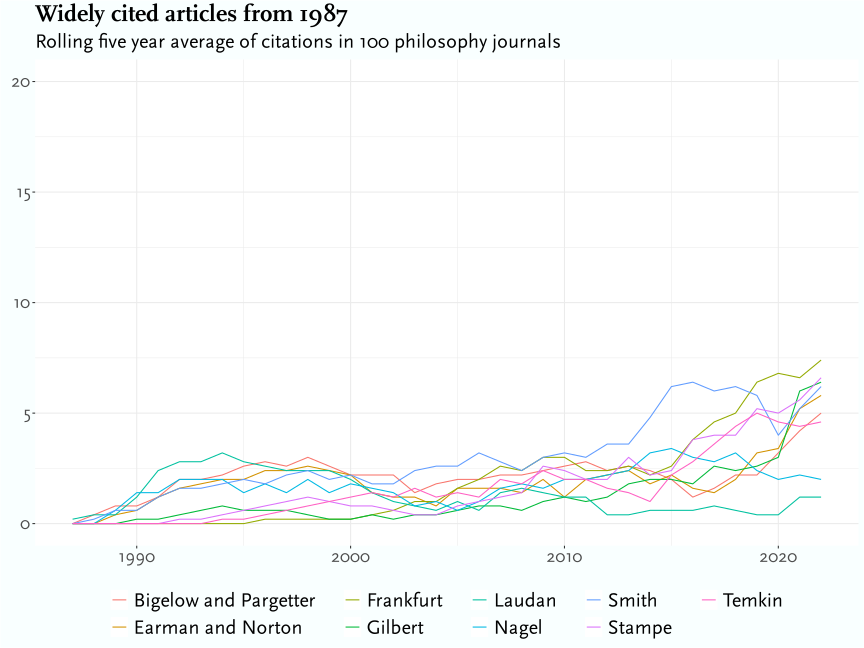
\includegraphics{citations_files/figure-pdf/fig-citation-spaghetti-1987-1.pdf}

}

\caption{\label{fig-citation-spaghetti-1987}Rolling five year average of
citation frequency for widely cited articles from 1987.}

\end{figure}%

\begin{figure}

\centering{

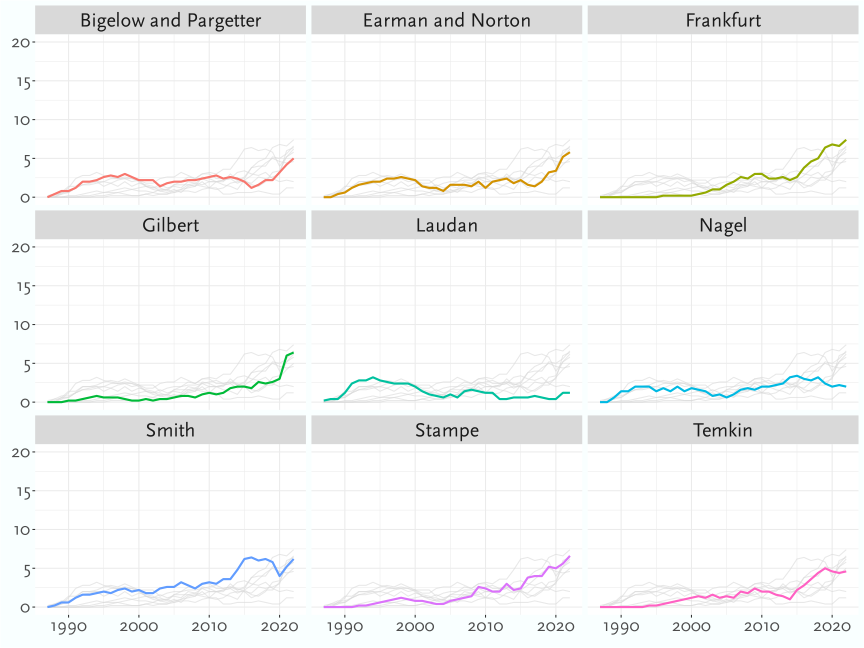
\includegraphics{citations_files/figure-pdf/fig-citation-facet-1987-1.pdf}

}

\caption{\label{fig-citation-facet-1987}Faceted version of
Figure~\ref{fig-citation-spaghetti-1987}.}

\end{figure}%

\newpage

\subsection{1988}\label{section-12}

\subsubsection*{Widely Cited Articles}\label{widely-cited-articles-12}
\addcontentsline{toc}{subsubsection}{Widely Cited Articles}

\begin{enumerate}
\def\labelenumi{\arabic{enumi}.}
\tightlist
\item
  T Burge, ``Individualism and Self-Knowledge'' \emph{Journal Of
  Philosophy} 85 (11): 649-663.
\item
  J Bogen and J Woodward, ``Saving the Phenomena'' \emph{Philosophical
  Review} 97 (3): 303-352.
\item
  A Grove, ``Two Modelings for Theory Change'' \emph{Journal Of
  Philosophical Logic} 17 (2): 157-170.
\item
  K Sterelny and P Kitcher, ``The Return of the Gene'' \emph{Journal Of
  Philosophy} 85 (7): 339-361.
\item
  S Kagan, ``The Additive Fallacy'' \emph{Ethics} 99 (1): 5-31.
\item
  WP Alston, ``An Internalist Externalism'' \emph{Synthese} 74 (3):
  265-283.
\item
  DLM Baxter, ``Identity in the Loose and Popular Sense'' \emph{Mind} 97
  (388): 575-582.
\item
  F Jackson and P Pettit, ``Functionalism and Broad Content''
  \emph{Mind} 97 (387): 381-400.
\item
  J Rawls, ``The Priority of Right and Ideas of the Good''
  \emph{Philosophy \& Public Affairs} 17 (4): 251-276.
\end{enumerate}

\subsubsection*{Citation Count}\label{citation-count-12}
\addcontentsline{toc}{subsubsection}{Citation Count}

\begin{longtable}[]{@{}lrrr@{}}

\caption{\label{tbl-citation-count-1988}Citation count for widely cited
articles from 1988.}

\tabularnewline

\toprule\noalign{}
Article & All & Early & Late \\
\midrule\noalign{}
\endhead
\bottomrule\noalign{}
\endlastfoot
Burge & 173 & 27 & 52 \\
Bogen and Woodward & 155 & 19 & 83 \\
Grove & 95 & 4 & 51 \\
Sterelny and Kitcher & 81 & 20 & 19 \\
Kagan & 76 & 11 & 39 \\
Alston & 71 & 7 & 44 \\
Jackson and Pettit & 66 & 34 & 9 \\
Baxter & 61 & 4 & 39 \\
Rawls & 37 & 23 & 10 \\

\end{longtable}

\subsubsection*{Citation Rank}\label{citation-rank-12}
\addcontentsline{toc}{subsubsection}{Citation Rank}

\begin{longtable}[]{@{}lrrr@{}}

\caption{\label{tbl-citation-rank-1988}Citation rank for widely cited
articles from 1988.}

\tabularnewline

\toprule\noalign{}
Article & Overall & Early & Late \\
\midrule\noalign{}
\endhead
\bottomrule\noalign{}
\endlastfoot
Burge & 1 & 2 & 2 \\
Bogen and Woodward & 2 & 5 & 1 \\
Grove & 3 & 64 & 3 \\
Sterelny and Kitcher & 4 & 4 & 16 \\
Kagan & 5 & 14 & 5 \\
Alston & 6 & 29 & 4 \\
Jackson and Pettit & 7 & 1 & 47 \\
Baxter & 10 & 64 & 5 \\
Rawls & 23 & 3 & 40 \\

\end{longtable}

\subsubsection*{Citation Trends}\label{citation-trends-12}
\addcontentsline{toc}{subsubsection}{Citation Trends}

\begin{figure}

\centering{

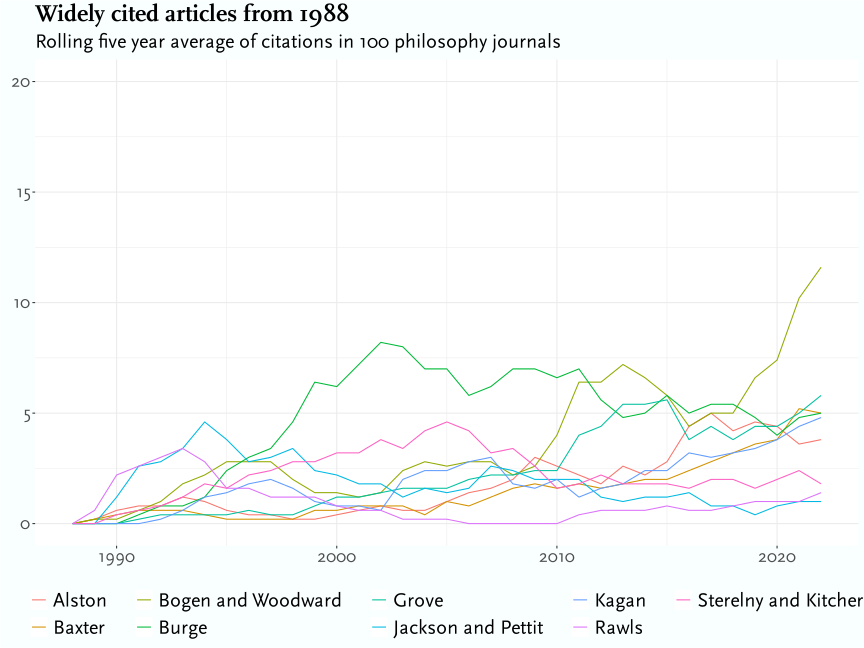
\includegraphics{citations_files/figure-pdf/fig-citation-spaghetti-1988-1.pdf}

}

\caption{\label{fig-citation-spaghetti-1988}Rolling five year average of
citation frequency for widely cited articles from 1988.}

\end{figure}%

\begin{figure}

\centering{

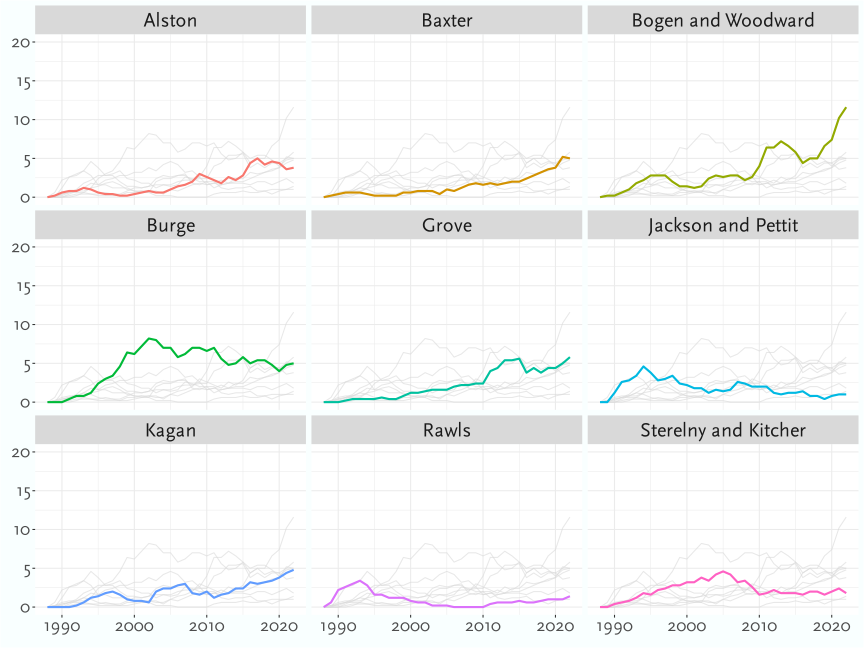
\includegraphics{citations_files/figure-pdf/fig-citation-facet-1988-1.pdf}

}

\caption{\label{fig-citation-facet-1988}Faceted version of
Figure~\ref{fig-citation-spaghetti-1988}.}

\end{figure}%

\newpage

\subsection{1989}\label{section-13}

\subsubsection*{Widely Cited Articles}\label{widely-cited-articles-13}
\addcontentsline{toc}{subsubsection}{Widely Cited Articles}

\begin{enumerate}
\def\labelenumi{\arabic{enumi}.}
\tightlist
\item
  GA Cohen, ``On the Currency of Egalitarian Justice'' \emph{Ethics} 99
  (4): 906-944.
\item
  RG Millikan, ``In Defense of Proper Functions'' \emph{Philosophy Of
  Science} 56 (2): 288-302.
\item
  RG Millikan, ``Biosemantics'' \emph{Journal Of Philosophy} 86 (6):
  281-297.
\item
  PA Boghossian and JD Velleman, ``Color as a Secondary Quality''
  \emph{Mind} 98 (389): 81-103.
\item
  RJ Arneson, ``Equality and Equal-Opportunity for Welfare''
  \emph{Philosophical Studies} 56 (1): 77-93.
\item
  PA Boghossian, ``The Rule-Following Considerations'' \emph{Mind} 5 98
  (392): 507-549.
\item
  WS Quinn, ``Actions, Intentions, and Consequences: The Doctrine of
  Double Effect'' \emph{Philosophy \& Public Affairs} 18 (4): 334-351.
\item
  D Marquis, ``Why Abortion is Immoral'' \emph{Journal Of Philosophy} 86
  (4): 183-202.
\item
  M Crimmins and J Perry, ``The Prince and the Phone Booth: Reporting
  Puzzling Beliefs'' \emph{Journal Of Philosophy} 86 (12): 685-711.
\end{enumerate}

\subsubsection*{Citation Count}\label{citation-count-13}
\addcontentsline{toc}{subsubsection}{Citation Count}

\begin{longtable}[]{@{}lrrr@{}}

\caption{\label{tbl-citation-count-1989}Citation count for widely cited
articles from 1989.}

\tabularnewline

\toprule\noalign{}
Article & All & Early & Late \\
\midrule\noalign{}
\endhead
\bottomrule\noalign{}
\endlastfoot
Cohen & 244 & 27 & 109 \\
Millikan, Proper Function & 173 & 35 & 86 \\
Millikan, Biosemantics & 164 & 32 & 89 \\
Boghossian and Velleman & 150 & 23 & 66 \\
Arneson & 138 & 11 & 65 \\
Boghossian & 107 & 14 & 43 \\
Crimmins and Perry & 90 & 25 & 39 \\
Marquis & 89 & 7 & 47 \\
Quinn & 79 & 15 & 47 \\

\end{longtable}

\subsubsection*{Citation Rank}\label{citation-rank-13}
\addcontentsline{toc}{subsubsection}{Citation Rank}

\begin{longtable}[]{@{}lrrr@{}}

\caption{\label{tbl-citation-rank-1989}Citation rank for widely cited
articles from 1989.}

\tabularnewline

\toprule\noalign{}
Article & Overall & Early & Late \\
\midrule\noalign{}
\endhead
\bottomrule\noalign{}
\endlastfoot
Cohen & 1 & 3 & 1 \\
Millikan, Proper Function & 2 & 1 & 3 \\
Millikan, Biosemantics & 3 & 2 & 2 \\
Boghossian and Velleman & 4 & 5 & 4 \\
Arneson & 5 & 15 & 5 \\
Boghossian & 6 & 8 & 10 \\
Crimmins and Perry & 8 & 4 & 11 \\
Marquis & 9 & 31 & 6 \\
Quinn & 10 & 7 & 6 \\

\end{longtable}

\subsubsection*{Citation Trends}\label{citation-trends-13}
\addcontentsline{toc}{subsubsection}{Citation Trends}

\begin{figure}

\centering{

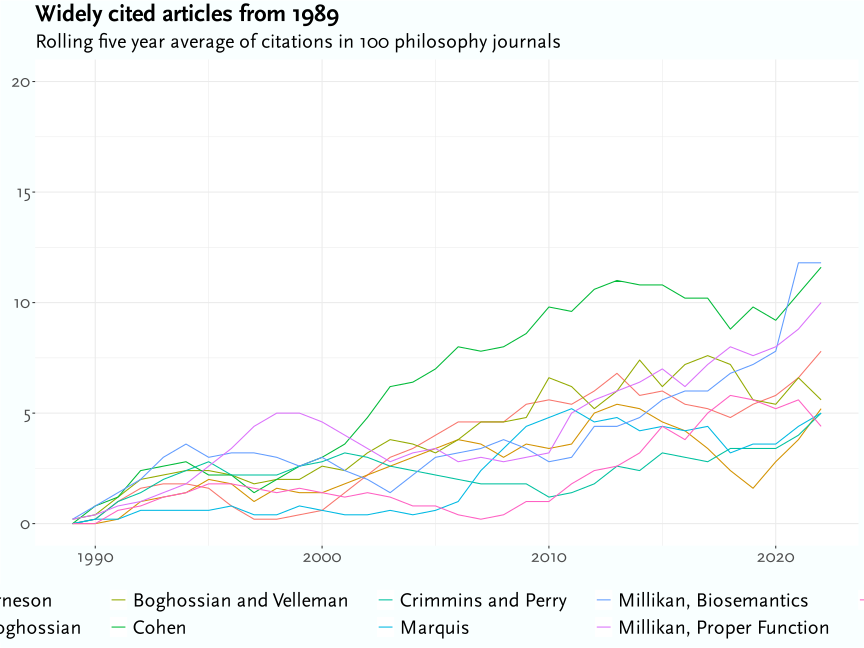
\includegraphics{citations_files/figure-pdf/fig-citation-spaghetti-1989-1.pdf}

}

\caption{\label{fig-citation-spaghetti-1989}Rolling five year average of
citation frequency for widely cited articles from 1989.}

\end{figure}%

\begin{figure}

\centering{

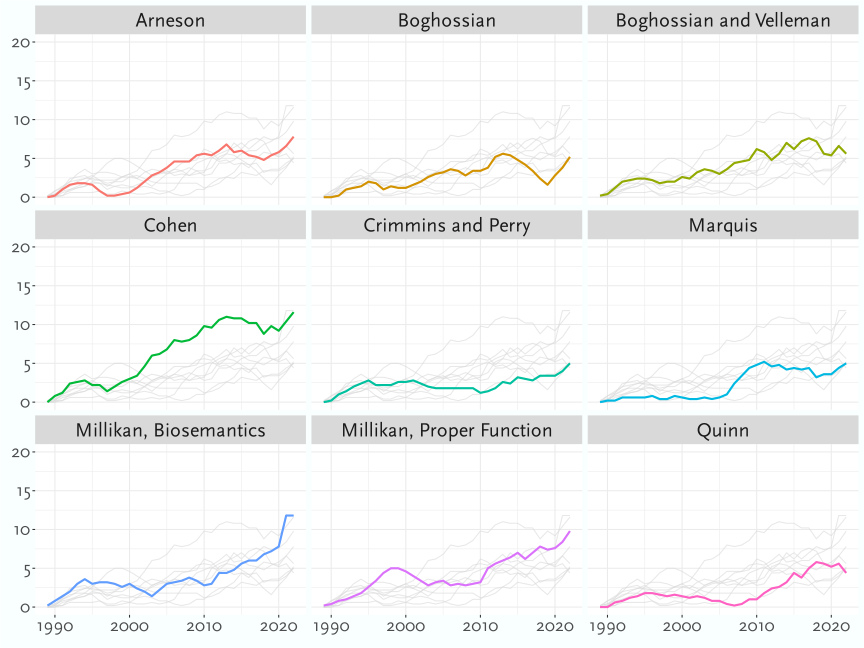
\includegraphics{citations_files/figure-pdf/fig-citation-facet-1989-1.pdf}

}

\caption{\label{fig-citation-facet-1989}Faceted version of
Figure~\ref{fig-citation-spaghetti-1989}.}

\end{figure}%

\newpage

\subsection{1990}\label{section-14}

\subsubsection*{Widely Cited Articles}\label{widely-cited-articles-14}
\addcontentsline{toc}{subsubsection}{Widely Cited Articles}

\begin{enumerate}
\def\labelenumi{\arabic{enumi}.}
\tightlist
\item
  P Kitcher, ``The Division of Cognitive Labor'' \emph{Journal Of
  Philosophy} 87 (1): 5-22.
\item
  F Jackson and P Pettit, ``Program Explanation: A General Perspective''
  \emph{Analysis} 50 (2): 107-117.
\item
  D Davidson, ``The Structure and Content of Truth'' \emph{Journal Of
  Philosophy} 87 (6): 279-328.
\item
  G Rosen, ``Modal Fictionalism'' \emph{Mind} 99 (395): 327-354.
\item
  T Crane and DH Mellor, ``There is No Question of Physicalism''
  \emph{Mind} 99 (394): 185-206.
\item
  J Vogel, ``Cartesian Skepticism and Inference To the Best
  Explanation'' \emph{Journal Of Philosophy} 87 (11): 658-666.
\item
  J Dreier, ``Internalism and Speaker Relativism'' \emph{Ethics} 101
  (1): 6-26.
\item
  JW Kim, ``Supervenience as a Philosophical Concept''
  \emph{Metaphilosophy} 21 (1-2): 1-27 -.
\item
  M Tye, ``Vague Objects'' \emph{Mind} 99 (396): 535-557.
\end{enumerate}

\subsubsection*{Citation Count}\label{citation-count-14}
\addcontentsline{toc}{subsubsection}{Citation Count}

\begin{longtable}[]{@{}lrrr@{}}

\caption{\label{tbl-citation-count-1990}Citation count for widely cited
articles from 1990.}

\tabularnewline

\toprule\noalign{}
Article & All & Early & Late \\
\midrule\noalign{}
\endhead
\bottomrule\noalign{}
\endlastfoot
Kitcher & 160 & 23 & 108 \\
Jackson and Pettit & 122 & 17 & 60 \\
Davidson & 114 & 40 & 29 \\
Rosen & 110 & 22 & 43 \\
Crane and Mellor & 95 & 30 & 30 \\
Dreier & 85 & 10 & 39 \\
Vogel & 76 & 8 & 46 \\
Kim & 59 & 23 & 21 \\
Tye & 51 & 22 & 12 \\

\end{longtable}

\subsubsection*{Citation Rank}\label{citation-rank-14}
\addcontentsline{toc}{subsubsection}{Citation Rank}

\begin{longtable}[]{@{}lrrr@{}}

\caption{\label{tbl-citation-rank-1990}Citation rank for widely cited
articles from 1990.}

\tabularnewline

\toprule\noalign{}
Article & Overall & Early & Late \\
\midrule\noalign{}
\endhead
\bottomrule\noalign{}
\endlastfoot
Kitcher & 1 & 3 & 1 \\
Jackson and Pettit & 2 & 9 & 2 \\
Davidson & 3 & 1 & 9 \\
Rosen & 4 & 5 & 4 \\
Crane and Mellor & 5 & 2 & 7 \\
Dreier & 7 & 16 & 5 \\
Vogel & 8 & 22 & 3 \\
Kim & 10 & 3 & 15 \\
Tye & 14 & 5 & 30 \\

\end{longtable}

\subsubsection*{Citation Trends}\label{citation-trends-14}
\addcontentsline{toc}{subsubsection}{Citation Trends}

\begin{figure}

\centering{

\includegraphics{citations_files/figure-pdf/fig-citation-spaghetti-1990-1.pdf}

}

\caption{\label{fig-citation-spaghetti-1990}Rolling five year average of
citation frequency for widely cited articles from 1990.}

\end{figure}%

\begin{figure}

\centering{

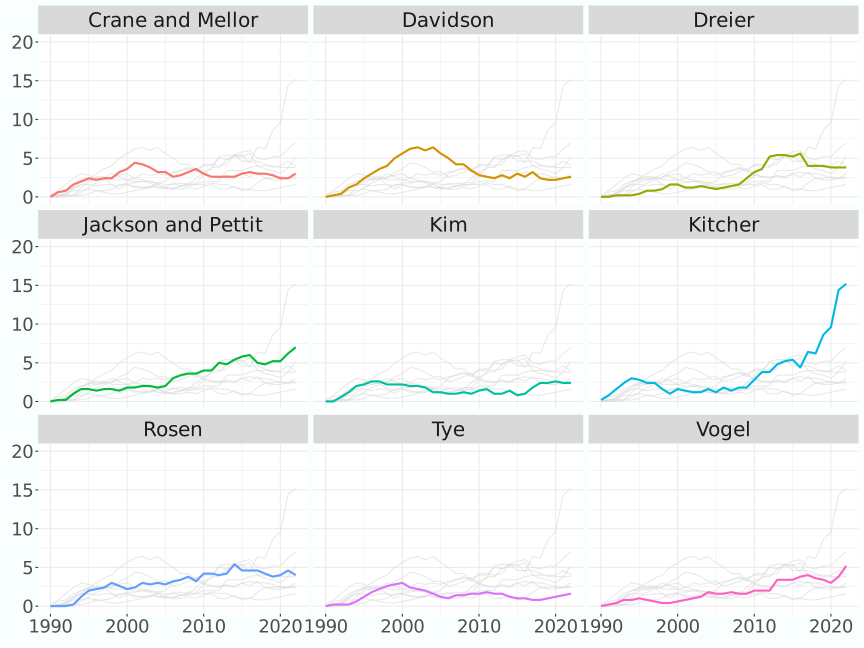
\includegraphics{citations_files/figure-pdf/fig-citation-facet-1990-1.pdf}

}

\caption{\label{fig-citation-facet-1990}Faceted version of
Figure~\ref{fig-citation-spaghetti-1990}.}

\end{figure}%

\newpage

\subsection{1991}\label{section-15}

\subsubsection*{Widely Cited Articles}\label{widely-cited-articles-15}
\addcontentsline{toc}{subsubsection}{Widely Cited Articles}

\begin{enumerate}
\def\labelenumi{\arabic{enumi}.}
\tightlist
\item
  K Neander, ``Functions as Selected Effects: The Conceptual Analysts
  Defense'' \emph{Philosophy Of Science} 58 (2): 168-184.
\item
  DC Dennett, ``Real Patterns'' \emph{Journal Of Philosophy} 88 (1):
  27-51.
\item
  R Boyd, ``Realism, Antifoundationalism and the Enthusiasm for Natural
  Kinds'' \emph{Philosophical Studies} 61 (1-2): 127-148.
\item
  F Jackson, ``Decision-Theoretic Consequentialism and the Nearest and
  Dearest Objection'' \emph{Ethics} 101 (3): 461-482.
\item
  JJ Thomson, ``Self-Defense'' \emph{Philosophy \& Public Affairs} 20
  (4): 283-310.
\item
  K DeRose, ``Epistemic Possibilities'' \emph{Philosophical Review} 100
  (4): 581-605.
\item
  J Hardwig, ``The Role of Trust in Knowledge'' \emph{Journal Of
  Philosophy} 88 (12): 693-708.
\item
  M McKinsey, ``Anti-Individualism and Privileged Access''
  \emph{Analysis} 51 (1): 9-16.
\item
  S Schiffer, ``Ceteris-Paribus Laws'' \emph{Mind} 100 (397): 1-17.
\end{enumerate}

\subsubsection*{Citation Count}\label{citation-count-15}
\addcontentsline{toc}{subsubsection}{Citation Count}

\begin{longtable}[]{@{}lrrr@{}}

\caption{\label{tbl-citation-count-1991}Citation count for widely cited
articles from 1991.}

\tabularnewline

\toprule\noalign{}
Article & All & Early & Late \\
\midrule\noalign{}
\endhead
\bottomrule\noalign{}
\endlastfoot
Neander & 190 & 41 & 94 \\
Dennett & 175 & 20 & 114 \\
Boyd & 154 & 8 & 103 \\
Jackson & 146 & 10 & 103 \\
Thomson & 127 & 7 & 63 \\
Derose & 113 & 10 & 63 \\
Hardwig & 99 & 10 & 63 \\
McKinsey & 86 & 25 & 23 \\
Schiffer & 54 & 22 & 12 \\

\end{longtable}

\subsubsection*{Citation Rank}\label{citation-rank-15}
\addcontentsline{toc}{subsubsection}{Citation Rank}

\begin{longtable}[]{@{}lrrr@{}}

\caption{\label{tbl-citation-rank-1991}Citation rank for widely cited
articles from 1991.}

\tabularnewline

\toprule\noalign{}
Article & Overall & Early & Late \\
\midrule\noalign{}
\endhead
\bottomrule\noalign{}
\endlastfoot
Neander & 1 & 1 & 4 \\
Dennett & 2 & 5 & 1 \\
Boyd & 3 & 31 & 2 \\
Jackson & 4 & 19 & 2 \\
Thomson & 5 & 43 & 5 \\
Derose & 6 & 19 & 5 \\
Hardwig & 7 & 19 & 5 \\
McKinsey & 10 & 2 & 18 \\
Schiffer & 17 & 3 & 39 \\

\end{longtable}

\subsubsection*{Citation Trends}\label{citation-trends-15}
\addcontentsline{toc}{subsubsection}{Citation Trends}

\begin{figure}

\centering{

\includegraphics{citations_files/figure-pdf/fig-citation-spaghetti-1991-1.pdf}

}

\caption{\label{fig-citation-spaghetti-1991}Rolling five year average of
citation frequency for widely cited articles from 1991.}

\end{figure}%

\begin{figure}

\centering{

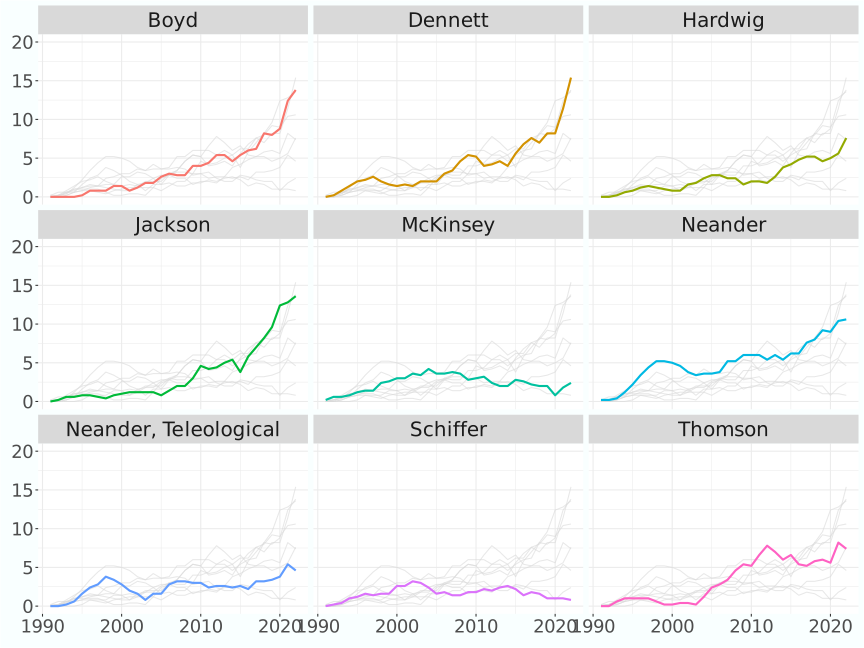
\includegraphics{citations_files/figure-pdf/fig-citation-facet-1991-1.pdf}

}

\caption{\label{fig-citation-facet-1991}Faceted version of
Figure~\ref{fig-citation-spaghetti-1991}.}

\end{figure}%

\newpage

\subsection{1992}\label{section-16}

\subsubsection*{Widely Cited Articles}\label{widely-cited-articles-16}
\addcontentsline{toc}{subsubsection}{Widely Cited Articles}

\begin{enumerate}
\def\labelenumi{\arabic{enumi}.}
\tightlist
\item
  S Yablo, ``Mental Causation'' \emph{Philosophical Review} 101 (2):
  245-280.
\item
  M Johnston, ``How To Speak of the Colors'' \emph{Philosophical
  Studies} 68 (3): 221-263.
\item
  K DeRose, ``Contextualism and Knowledge Attributions''
  \emph{Philosophy And Phenomenological Research} 52 (4): 913-929.
\item
  JW Kim, ``Multiple Realization and the Metaphysics of Reduction''
  \emph{Philosophy And Phenomenological Research} 52 (1): 1-26.
\item
  ME Bratman, ``Shared Cooperative Activity'' \emph{Philosophical
  Review} 101 (2): 327-340.
\item
  R Foley, ``The Epistemology of Belief and the Epistemology of Degrees
  of Belief'' \emph{American Philosophical Quarterly} 29 (2): 111-124.
\item
  MB Burke, ``Copper Statues and Pieces of Copper: A Challenge To the
  Standard Account'' \emph{Analysis} 52 (1): 12-17.
\item
  P Kitcher, ``The Naturalists Return'' \emph{Philosophical Review} 101
  (1): 53-114.
\item
  A Brueckner, ``What An Antiindividualist Knows A-Priori''
  \emph{Analysis} 52 (2): 111-118.
\end{enumerate}

\subsubsection*{Citation Count}\label{citation-count-16}
\addcontentsline{toc}{subsubsection}{Citation Count}

\begin{longtable}[]{@{}lrrr@{}}

\caption{\label{tbl-citation-count-1992}Citation count for widely cited
articles from 1992.}

\tabularnewline

\toprule\noalign{}
Article & All & Early & Late \\
\midrule\noalign{}
\endhead
\bottomrule\noalign{}
\endlastfoot
Yablo & 300 & 51 & 148 \\
Johnston & 261 & 30 & 142 \\
Derose & 246 & 12 & 139 \\
Kim & 125 & 23 & 54 \\
Bratman & 88 & 5 & 59 \\
Kitcher & 86 & 25 & 27 \\
Foley & 78 & 5 & 59 \\
Burke & 74 & 27 & 25 \\
Brueckner & 34 & 25 & 3 \\

\end{longtable}

\subsubsection*{Citation Rank}\label{citation-rank-16}
\addcontentsline{toc}{subsubsection}{Citation Rank}

\begin{longtable}[]{@{}lrrr@{}}

\caption{\label{tbl-citation-rank-1992}Citation rank for widely cited
articles from 1992.}

\tabularnewline

\toprule\noalign{}
Article & Overall & Early & Late \\
\midrule\noalign{}
\endhead
\bottomrule\noalign{}
\endlastfoot
Yablo & 1 & 1 & 1 \\
Johnston & 2 & 2 & 2 \\
Derose & 3 & 15 & 3 \\
Kim & 4 & 6 & 6 \\
Bratman & 5 & 70 & 4 \\
Kitcher & 6 & 4 & 20 \\
Foley & 10 & 70 & 4 \\
Burke & 12 & 3 & 23 \\
Brueckner & 32 & 4 & 155 \\

\end{longtable}

\subsubsection*{Citation Trends}\label{citation-trends-16}
\addcontentsline{toc}{subsubsection}{Citation Trends}

\begin{figure}

\centering{

\includegraphics{citations_files/figure-pdf/fig-citation-spaghetti-1992-1.pdf}

}

\caption{\label{fig-citation-spaghetti-1992}Rolling five year average of
citation frequency for widely cited articles from 1992.}

\end{figure}%

\begin{figure}

\centering{

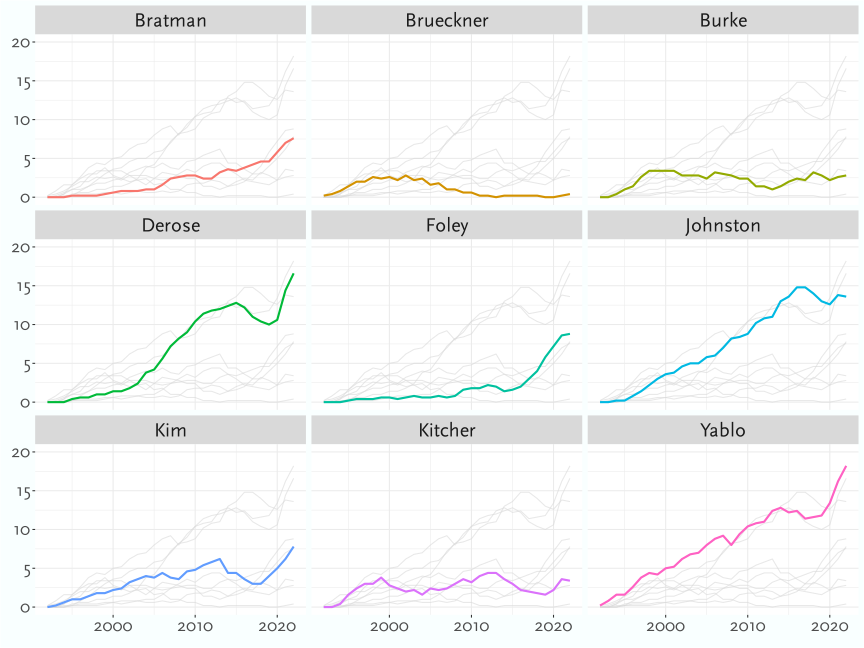
\includegraphics{citations_files/figure-pdf/fig-citation-facet-1992-1.pdf}

}

\caption{\label{fig-citation-facet-1992}Faceted version of
Figure~\ref{fig-citation-spaghetti-1992}.}

\end{figure}%

\newpage

\subsection{1993}\label{section-17}

\subsubsection*{Widely Cited Articles}\label{widely-cited-articles-17}
\addcontentsline{toc}{subsubsection}{Widely Cited Articles}

\begin{enumerate}
\def\labelenumi{\arabic{enumi}.}
\tightlist
\item
  T Burge, ``Content Preservation'' \emph{Philosophical Review} 102 (4):
  457-488.
\item
  S Yablo, ``Is Conceivability a Guide To Possibility'' \emph{Philosophy
  And Phenomenological Research} 53 (1): 1-42.
\item
  R Langton, ``Speech Acts and Unspeakable Acts'' \emph{Philosophy \&
  Public Affairs} 22 (4): 293-330.
\item
  S Yablo, ``Paradox Without Self-Reference'' \emph{Analysis} 53 (4):
  251-252.
\item
  ME Bratman, ``Shared Intention'' \emph{Ethics} 104 (1): 97-113.
\item
  PE Griffiths, ``Functional-Analysis and Proper Functions''
  \emph{British Journal For The Philosophy Of Science} 44 (3): 409-422.
\item
  J Dreier, ``Structures of Normative Theories'' \emph{Monist} 76 (1):
  22-40.
\item
  F Dretske, ``Conscious Experience'' \emph{Mind} 102 (406): 263-283.
\item
  RK Larson and P Ludlow, ``Interpreted Logical Forms'' \emph{Synthese}
  95 (3): 305-355.
\end{enumerate}

\subsubsection*{Citation Count}\label{citation-count-17}
\addcontentsline{toc}{subsubsection}{Citation Count}

\begin{longtable}[]{@{}lrrr@{}}

\caption{\label{tbl-citation-count-1993}Citation count for widely cited
articles from 1993.}

\tabularnewline

\toprule\noalign{}
Article & All & Early & Late \\
\midrule\noalign{}
\endhead
\bottomrule\noalign{}
\endlastfoot
Burge & 297 & 54 & 141 \\
Yablo, Conceivability & 159 & 18 & 106 \\
Langton & 103 & 6 & 84 \\
Yablo, Paradox & 95 & 19 & 47 \\
Bratman & 78 & 5 & 49 \\
Griffiths & 75 & 17 & 38 \\
Dretske & 66 & 21 & 21 \\
Dreier & 65 & 4 & 46 \\
Larson and Ludlow & 40 & 16 & 12 \\

\end{longtable}

\subsubsection*{Citation Rank}\label{citation-rank-17}
\addcontentsline{toc}{subsubsection}{Citation Rank}

\begin{longtable}[]{@{}lrrr@{}}

\caption{\label{tbl-citation-rank-1993}Citation rank for widely cited
articles from 1993.}

\tabularnewline

\toprule\noalign{}
Article & Overall & Early & Late \\
\midrule\noalign{}
\endhead
\bottomrule\noalign{}
\endlastfoot
Burge & 1 & 1 & 1 \\
Yablo, Conceivability & 2 & 4 & 2 \\
Langton & 3 & 47 & 3 \\
Yablo, Paradox & 4 & 3 & 5 \\
Bratman & 5 & 57 & 4 \\
Griffiths & 6 & 5 & 8 \\
Dretske & 9 & 2 & 15 \\
Dreier & 10 & 79 & 6 \\
Larson and Ludlow & 17 & 6 & 35 \\

\end{longtable}

\subsubsection*{Citation Trends}\label{citation-trends-17}
\addcontentsline{toc}{subsubsection}{Citation Trends}

\begin{figure}

\centering{

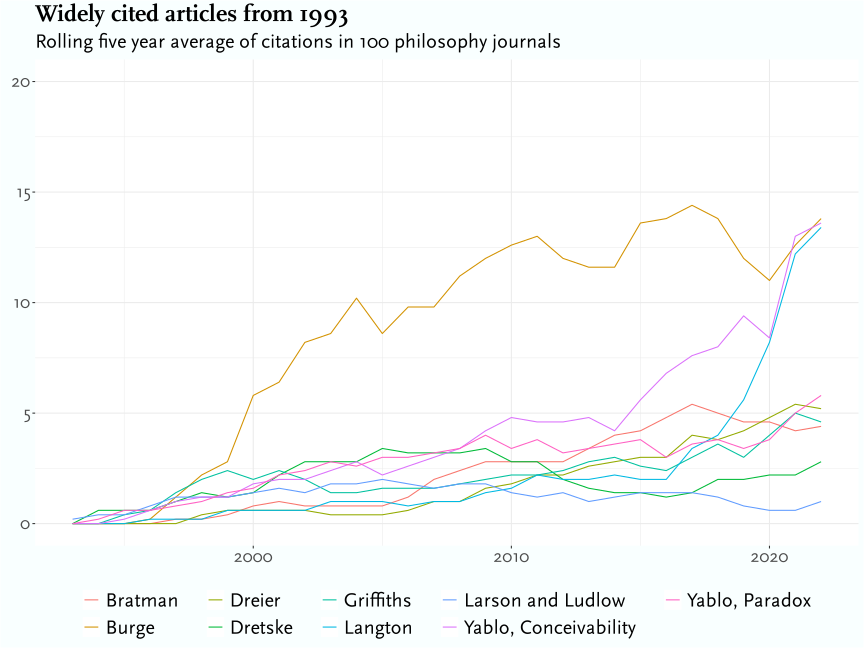
\includegraphics{citations_files/figure-pdf/fig-citation-spaghetti-1993-1.pdf}

}

\caption{\label{fig-citation-spaghetti-1993}Rolling five year average of
citation frequency for widely cited articles from 1993.}

\end{figure}%

\begin{figure}

\centering{

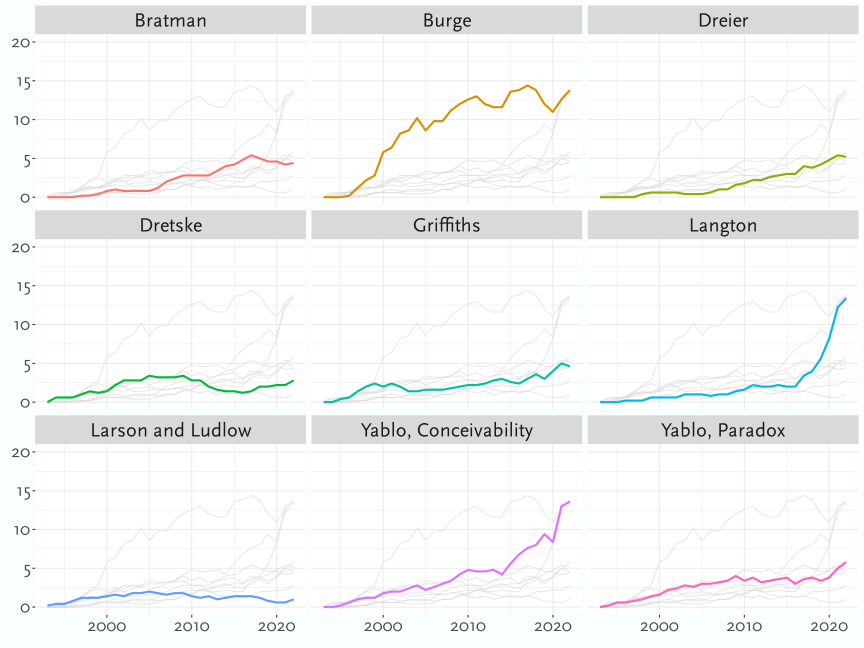
\includegraphics{citations_files/figure-pdf/fig-citation-facet-1993-1.pdf}

}

\caption{\label{fig-citation-facet-1993}Faceted version of
Figure~\ref{fig-citation-spaghetti-1993}.}

\end{figure}%

\newpage

\subsection{1994}\label{section-18}

\subsubsection*{Widely Cited Articles}\label{widely-cited-articles-18}
\addcontentsline{toc}{subsubsection}{Widely Cited Articles}

\begin{enumerate}
\def\labelenumi{\arabic{enumi}.}
\tightlist
\item
  D Lewis, ``Humean Supervenience Debugged'' \emph{Mind} 103 (412):
  473-490.
\item
  CB Martin, ``Dispositions and Conditionals'' \emph{Philosophical
  Quarterly} 44 (174): 1-8.
\item
  H Field, ``Deflationist Views of Meaning and Content'' \emph{Mind} 103
  (411): 249-285.
\item
  M Forster and E Sober, ``How To Tell When Simpler, More Unified, or
  Less Ad-Hoc Theories Will Provide More Accurate Predictions''
  \emph{British Journal For The Philosophy Of Science} 45 (1): 1-35.
\item
  P Godfrey-Smith, ``A Modern History Theory of Functions'' \emph{Noûs}
  28 (3): 344-362.
\item
  G Strawson, ``The Impossibility of Moral Responsibility''
  \emph{Philosophical Studies} 75 (1-2): 5-24.
\item
  R Audi, ``Dispositional Beliefs and Dispositions To Believe''
  \emph{Noûs} 28 (4): 419-434.
\item
  R Holton, ``Deciding To Trust, Coming To Believe'' \emph{Australasian
  Journal Of Philosophy} 72 (1): 63-76.
\item
  H Putnam, ``Sense, Nonsense, and the Senses: An Inquiry into the
  Powers of the Human Mind'' \emph{Journal Of Philosophy} 91 (9):
  445-465.
\end{enumerate}

\subsubsection*{Citation Count}\label{citation-count-18}
\addcontentsline{toc}{subsubsection}{Citation Count}

\begin{longtable}[]{@{}lrrr@{}}

\caption{\label{tbl-citation-count-1994}Citation count for widely cited
articles from 1994.}

\tabularnewline

\toprule\noalign{}
Article & All & Early & Late \\
\midrule\noalign{}
\endhead
\bottomrule\noalign{}
\endlastfoot
Lewis & 297 & 40 & 193 \\
Martin & 203 & 33 & 95 \\
Field & 135 & 42 & 64 \\
Forster and Sober & 125 & 37 & 59 \\
Godfrey-Smith & 108 & 24 & 55 \\
Audi & 102 & 7 & 69 \\
Strawson & 97 & 11 & 72 \\
Holton & 84 & 5 & 67 \\
Putnam & 67 & 38 & 17 \\

\end{longtable}

\subsubsection*{Citation Rank}\label{citation-rank-18}
\addcontentsline{toc}{subsubsection}{Citation Rank}

\begin{longtable}[]{@{}lrrr@{}}

\caption{\label{tbl-citation-rank-1994}Citation rank for widely cited
articles from 1994.}

\tabularnewline

\toprule\noalign{}
Article & Overall & Early & Late \\
\midrule\noalign{}
\endhead
\bottomrule\noalign{}
\endlastfoot
Lewis & 1 & 2 & 1 \\
Martin & 2 & 6 & 2 \\
Field & 3 & 1 & 6 \\
Forster and Sober & 4 & 4 & 8 \\
Godfrey-Smith & 5 & 12 & 9 \\
Audi & 6 & 61 & 4 \\
Strawson & 7 & 31 & 3 \\
Holton & 10 & 97 & 5 \\
Putnam & 19 & 3 & 40 \\

\end{longtable}

\subsubsection*{Citation Trends}\label{citation-trends-18}
\addcontentsline{toc}{subsubsection}{Citation Trends}

\begin{figure}

\centering{

\includegraphics{citations_files/figure-pdf/fig-citation-spaghetti-1994-1.pdf}

}

\caption{\label{fig-citation-spaghetti-1994}Rolling five year average of
citation frequency for widely cited articles from 1994.}

\end{figure}%

\begin{figure}

\centering{

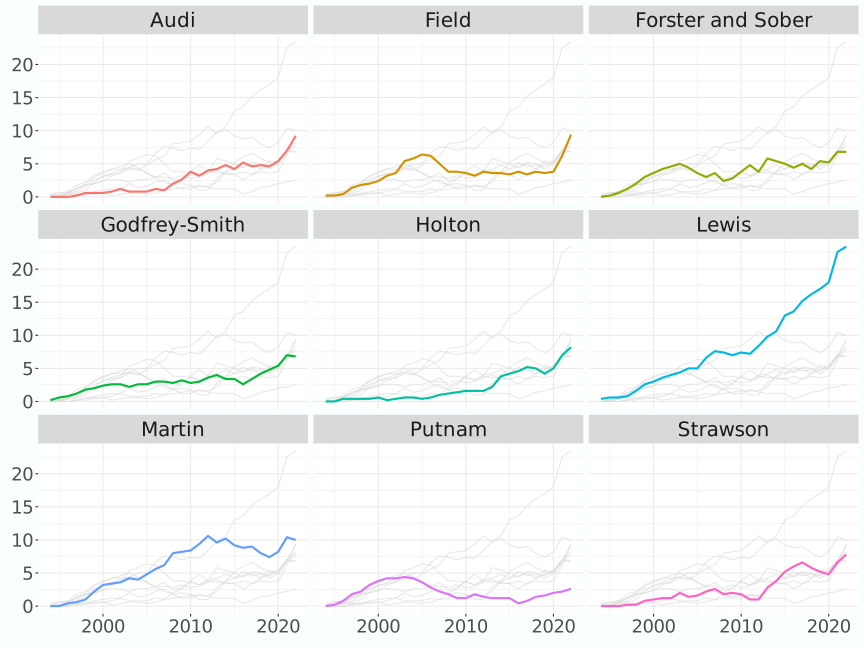
\includegraphics{citations_files/figure-pdf/fig-citation-facet-1994-1.pdf}

}

\caption{\label{fig-citation-facet-1994}Faceted version of
Figure~\ref{fig-citation-spaghetti-1994}.}

\end{figure}%

\newpage

\subsection{1995}\label{section-19}

\subsubsection*{Widely Cited Articles}\label{widely-cited-articles-19}
\addcontentsline{toc}{subsubsection}{Widely Cited Articles}

\begin{enumerate}
\def\labelenumi{\arabic{enumi}.}
\tightlist
\item
  K DeRose, ``Solving the Skeptical Problem'' \emph{Philosophical
  Review} 104 (1): 1-52.
\item
  D Widerker, ``Libertarianism and Frankfurt's Attack on the Principle
  of Alternative Possibilities'' \emph{Philosophical Review} 104 (2):
  247-261.
\item
  DW Zimmerman, ``Theories of Masses and Problems of Constitution''
  \emph{Philosophical Review} 104 (1): 53-110.
\item
  T van Gelder, ``What Might Cognition Be, If Not Computation''
  \emph{Journal Of Philosophy} 92 (7): 345-381.
\item
  K Neander, ``Misrepresenting and Malfunctioning'' \emph{Philosophical
  Studies} 79 (2): 109-141.
\item
  P Pietroski and G Rey, ``When Other Things Arent Equal: Saving Ceteris
  Paribus Laws From Vacuity'' \emph{British Journal For The Philosophy
  Of Science} 46 (1): 81-110.
\item
  K Fine, ``The Logic of Essence'' \emph{Journal Of Philosophical Logic}
  24 (3): 241-273.
\item
  J McDowell, ``Knowledge and the Internal'' \emph{Philosophy And
  Phenomenological Research} 55 (4): 877-893.
\item
  N Chomsky, ``Language and Nature'' \emph{Mind} 104 (413): 1-61.
\end{enumerate}

\subsubsection*{Citation Count}\label{citation-count-19}
\addcontentsline{toc}{subsubsection}{Citation Count}

\begin{longtable}[]{@{}lrrr@{}}

\caption{\label{tbl-citation-count-1995}Citation count for widely cited
articles from 1995.}

\tabularnewline

\toprule\noalign{}
Article & All & Early & Late \\
\midrule\noalign{}
\endhead
\bottomrule\noalign{}
\endlastfoot
Derose & 316 & 84 & 124 \\
Widerker & 96 & 26 & 35 \\
Zimmerman & 90 & 36 & 29 \\
Gelder & 83 & 13 & 56 \\
Neander & 83 & 26 & 42 \\
Pietroski and Rey & 80 & 25 & 33 \\
McDowell & 78 & 8 & 49 \\
Chomsky & 74 & 21 & 39 \\
Fine & 62 & 3 & 55 \\

\end{longtable}

\subsubsection*{Citation Rank}\label{citation-rank-19}
\addcontentsline{toc}{subsubsection}{Citation Rank}

\begin{longtable}[]{@{}lrrr@{}}

\caption{\label{tbl-citation-rank-1995}Citation rank for widely cited
articles from 1995.}

\tabularnewline

\toprule\noalign{}
Article & Overall & Early & Late \\
\midrule\noalign{}
\endhead
\bottomrule\noalign{}
\endlastfoot
Derose & 1 & 1 & 1 \\
Widerker & 2 & 3 & 8 \\
Zimmerman & 3 & 2 & 13 \\
Gelder & 4 & 17 & 2 \\
Neander & 4 & 3 & 5 \\
Pietroski and Rey & 6 & 5 & 11 \\
McDowell & 7 & 40 & 4 \\
Chomsky & 8 & 8 & 6 \\
Fine & 11 & 142 & 3 \\

\end{longtable}

\subsubsection*{Citation Trends}\label{citation-trends-19}
\addcontentsline{toc}{subsubsection}{Citation Trends}

\begin{figure}

\centering{

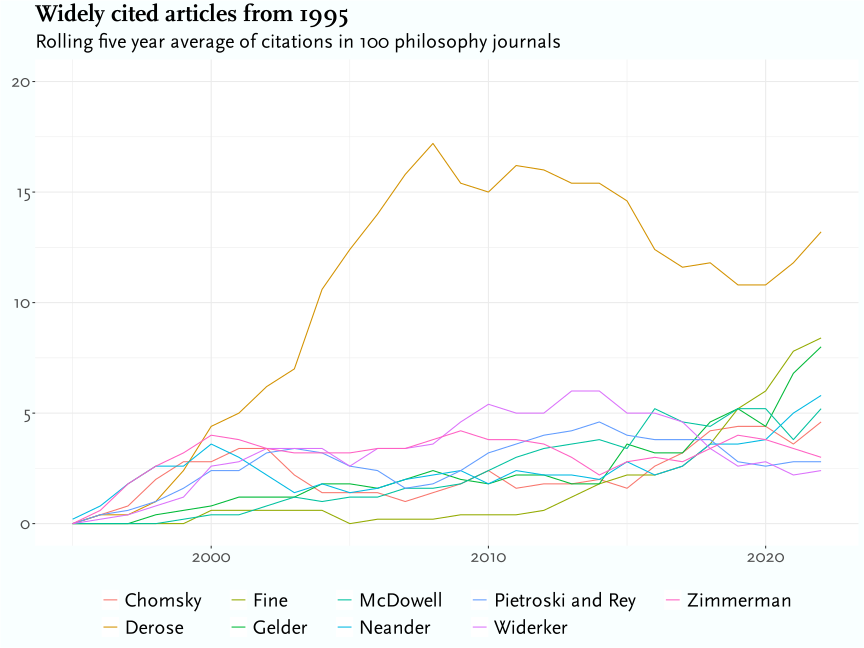
\includegraphics{citations_files/figure-pdf/fig-citation-spaghetti-1995-1.pdf}

}

\caption{\label{fig-citation-spaghetti-1995}Rolling five year average of
citation frequency for widely cited articles from 1995.}

\end{figure}%

\begin{figure}

\centering{

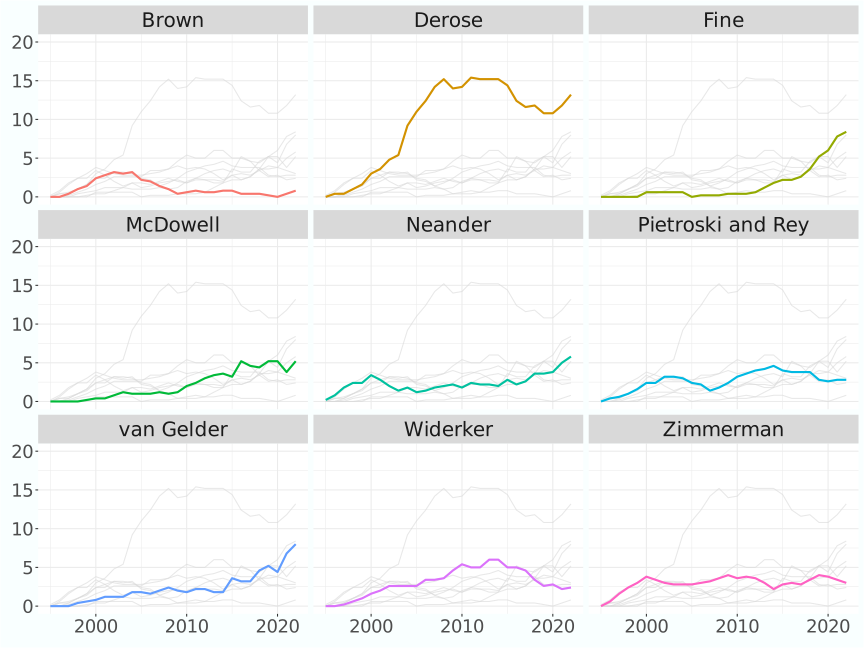
\includegraphics{citations_files/figure-pdf/fig-citation-facet-1995-1.pdf}

}

\caption{\label{fig-citation-facet-1995}Faceted version of
Figure~\ref{fig-citation-spaghetti-1995}.}

\end{figure}%

\newpage

\subsection{1996}\label{section-20}

\subsubsection*{Widely Cited Articles}\label{widely-cited-articles-20}
\addcontentsline{toc}{subsubsection}{Widely Cited Articles}

\begin{enumerate}
\def\labelenumi{\arabic{enumi}.}
\tightlist
\item
  D Lewis, ``Elusive Knowledge'' \emph{Australasian Journal Of
  Philosophy} 74 (4): 549-567.
\item
  T Williamson, ``Knowing and Asserting'' \emph{Philosophical Review}
  105 (4): 489-523.
\item
  F Veltman, ``Defaults in Update Semantics'' \emph{Journal Of
  Philosophical Logic} 25 (3): 221-261.
\item
  K Jones, ``Trust as An Affective Attitude'' \emph{Ethics} 107 (1):
  4-25.
\item
  R Dworkin, ``Objectivity and Truth: You'd Better Believe It''
  \emph{Philosophy \& Public Affairs} 25 (2): 87-139.
\item
  D Davidson, ``The Folly of Trying To Define Truth'' \emph{Journal Of
  Philosophy} 93 (6): 263-278.
\item
  A Oliver, ``The Metaphysics of Properties'' \emph{Mind} 105 (417):
  1-80.
\item
  T Sider, ``All the World's a Stage'' \emph{Australasian Journal Of
  Philosophy} 74 (3): 433-453.
\item
  C McGinn, ``Another Look At Color'' \emph{Journal Of Philosophy} 93
  (11): 537-553.
\end{enumerate}

\subsubsection*{Citation Count}\label{citation-count-20}
\addcontentsline{toc}{subsubsection}{Citation Count}

\begin{longtable}[]{@{}lrrr@{}}

\caption{\label{tbl-citation-count-1996}Citation count for widely cited
articles from 1996.}

\tabularnewline

\toprule\noalign{}
Article & All & Early & Late \\
\midrule\noalign{}
\endhead
\bottomrule\noalign{}
\endlastfoot
Lewis & 505 & 117 & 277 \\
Williamson & 155 & 21 & 109 \\
Veltman & 120 & 7 & 99 \\
Jones & 104 & 4 & 81 \\
Dworkin & 100 & 18 & 67 \\
Sider & 86 & 20 & 47 \\
McGinn & 72 & 20 & 32 \\
Oliver & 65 & 21 & 34 \\
Davidson & 60 & 28 & 21 \\

\end{longtable}

\subsubsection*{Citation Rank}\label{citation-rank-20}
\addcontentsline{toc}{subsubsection}{Citation Rank}

\begin{longtable}[]{@{}lrrr@{}}

\caption{\label{tbl-citation-rank-1996}Citation rank for widely cited
articles from 1996.}

\tabularnewline

\toprule\noalign{}
Article & Overall & Early & Late \\
\midrule\noalign{}
\endhead
\bottomrule\noalign{}
\endlastfoot
Lewis & 1 & 1 & 1 \\
Williamson & 2 & 3 & 2 \\
Veltman & 3 & 55 & 3 \\
Jones & 4 & 122 & 4 \\
Dworkin & 5 & 8 & 5 \\
Sider & 7 & 5 & 8 \\
McGinn & 8 & 5 & 11 \\
Oliver & 10 & 3 & 10 \\
Davidson & 13 & 2 & 32 \\

\end{longtable}

\subsubsection*{Citation Trends}\label{citation-trends-20}
\addcontentsline{toc}{subsubsection}{Citation Trends}

\begin{figure}

\centering{

\includegraphics{citations_files/figure-pdf/fig-citation-spaghetti-1996-1.pdf}

}

\caption{\label{fig-citation-spaghetti-1996}Rolling five year average of
citation frequency for widely cited articles from 1996.}

\end{figure}%

\begin{figure}

\centering{

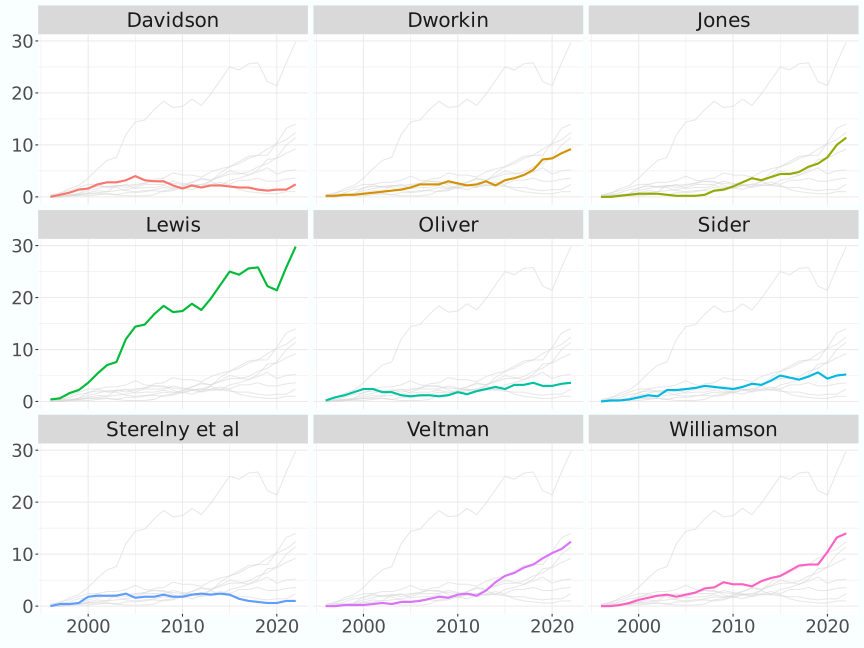
\includegraphics{citations_files/figure-pdf/fig-citation-facet-1996-1.pdf}

}

\caption{\label{fig-citation-facet-1996}Faceted version of
Figure~\ref{fig-citation-spaghetti-1996}.}

\end{figure}%

\newpage

\subsection{1997}\label{section-21}

\subsubsection*{Widely Cited Articles}\label{widely-cited-articles-21}
\addcontentsline{toc}{subsubsection}{Widely Cited Articles}

\begin{enumerate}
\def\labelenumi{\arabic{enumi}.}
\tightlist
\item
  D Lewis, ``Finkish Dispositions'' \emph{Philosophical Quarterly} 47
  (187): 143-158.
\item
  D Parfit, ``Equality and Priority'' \emph{Ratio-New Series} 10 (3):
  202-221.
\item
  LR Baker, ``Why Constitution is Not Identity'' \emph{Journal Of
  Philosophy} 94 (12): 599-621.
\item
  R Audi, ``The Place of Testimony in the Fabric of Knowledge and
  Justification'' \emph{American Philosophical Quarterly} 34 (4):
  405-422.
\item
  CS Hill, ``Imaginability, Conceivability, Possibility and the
  Mind-Body Problem'' \emph{Philosophical Studies} 87 (1): 61-85.
\item
  MJ Zimmerman, ``Moral Responsibility and Ignorance'' \emph{Ethics} 107
  (3): 410-426.
\item
  J Fodor, ``Special Sciences: Still Autonomous After All These Years''
  \emph{Noûs} 149-163.
\item
  T Sider, ``Four-Dimensionalism'' \emph{Philosophical Review} 106 (2):
  197-231.
\item
  T Burge, ``Interlocution, Perception, and Memory'' \emph{Philosophical
  Studies} 86 (1): 21-47.
\end{enumerate}

\subsubsection*{Citation Count}\label{citation-count-21}
\addcontentsline{toc}{subsubsection}{Citation Count}

\begin{longtable}[]{@{}lrrr@{}}

\caption{\label{tbl-citation-count-1997}Citation count for widely cited
articles from 1997.}

\tabularnewline

\toprule\noalign{}
Article & All & Early & Late \\
\midrule\noalign{}
\endhead
\bottomrule\noalign{}
\endlastfoot
Lewis & 217 & 41 & 121 \\
Parfit & 111 & 14 & 80 \\
Baker & 82 & 25 & 44 \\
Audi & 73 & 25 & 40 \\
Hill & 70 & 19 & 27 \\
Burge & 63 & 24 & 31 \\
Zimmerman & 57 & 5 & 47 \\
Fodor & 53 & 0 & 46 \\
Sider & 51 & 27 & 17 \\

\end{longtable}

\subsubsection*{Citation Rank}\label{citation-rank-21}
\addcontentsline{toc}{subsubsection}{Citation Rank}

\begin{longtable}[]{@{}lrrr@{}}

\caption{\label{tbl-citation-rank-1997}Citation rank for widely cited
articles from 1997.}

\tabularnewline

\toprule\noalign{}
Article & Overall & Early & Late \\
\midrule\noalign{}
\endhead
\bottomrule\noalign{}
\endlastfoot
Lewis & 1 & 1 & 1 \\
Parfit & 2 & 20 & 2 \\
Baker & 3 & 3 & 5 \\
Audi & 4 & 3 & 8 \\
Hill & 5 & 7 & 20 \\
Burge & 6 & 5 & 17 \\
Zimmerman & 14 & 102 & 3 \\
Fodor & 18 & 713 & 4 \\
Sider & 20 & 2 & 38 \\

\end{longtable}

\subsubsection*{Citation Trends}\label{citation-trends-21}
\addcontentsline{toc}{subsubsection}{Citation Trends}

\begin{figure}

\centering{

\includegraphics{citations_files/figure-pdf/fig-citation-spaghetti-1997-1.pdf}

}

\caption{\label{fig-citation-spaghetti-1997}Rolling five year average of
citation frequency for widely cited articles from 1997.}

\end{figure}%

\begin{figure}

\centering{

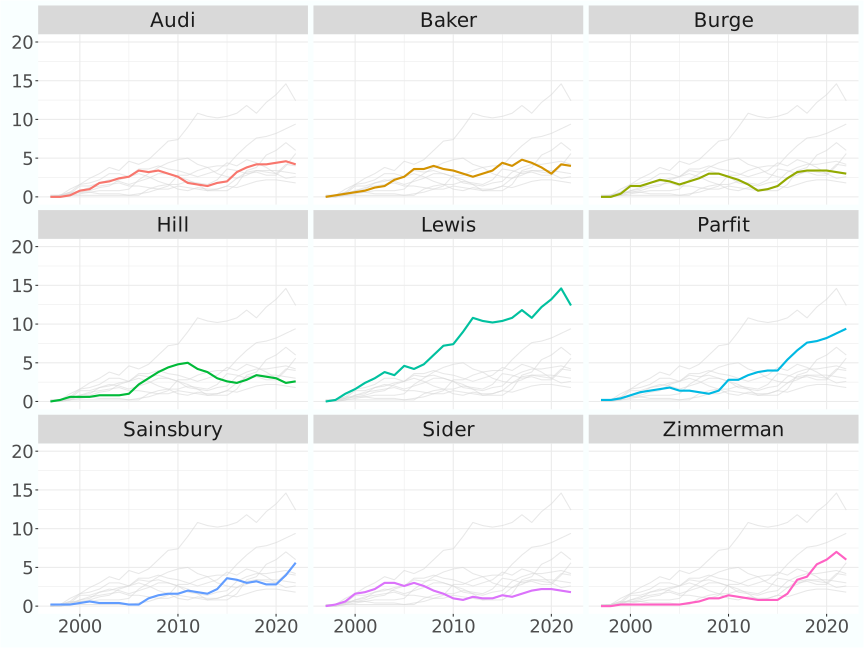
\includegraphics{citations_files/figure-pdf/fig-citation-facet-1997-1.pdf}

}

\caption{\label{fig-citation-facet-1997}Faceted version of
Figure~\ref{fig-citation-spaghetti-1997}.}

\end{figure}%

\newpage

\subsection{1998}\label{section-22}

\subsubsection*{Widely Cited Articles}\label{widely-cited-articles-22}
\addcontentsline{toc}{subsubsection}{Widely Cited Articles}

\begin{enumerate}
\def\labelenumi{\arabic{enumi}.}
\tightlist
\item
  A Clark and D Chalmers, ``The Extended Mind'' \emph{Analysis} 58 (1):
  7-19.
\item
  JM Joyce, ``A Nonpragmatic Vindication of Probabilism''
  \emph{Philosophy Of Science} 65 (4): 575-603.
\item
  J Ladyman, ``What is Structural Realism?'' \emph{Studies In History
  And Philosophy Of Science} 29 (3): 409-424.
\item
  A Bird, ``Dispositions and Antidotes'' \emph{Philosophical Quarterly}
  48 (191): 227-234.
\item
  N Salmon, ``Nonexistence'' \emph{Noûs} 32 (3): 277-319.
\item
  R Langton and D Lewis, ``Defining `Intrinsic'\,'' \emph{Philosophy And
  Phenomenological Research} 58 (2): 333-345.
\item
  E Conee and R Feldman, ``The Generality Problem for Reliabilism''
  \emph{Philosophical Studies} 89 (1): 1-29.
\item
  JJ Thomson, ``The Statue and the Clay'' \emph{Noûs} 32 (2): 149-173.
\item
  N Markosian, ``Brutal Composition'' \emph{Philosophical Studies} 92
  (3): 211-249.
\end{enumerate}

\subsubsection*{Citation Count}\label{citation-count-22}
\addcontentsline{toc}{subsubsection}{Citation Count}

\begin{longtable}[]{@{}lrrr@{}}

\caption{\label{tbl-citation-count-1998}Citation count for widely cited
articles from 1998.}

\tabularnewline

\toprule\noalign{}
Article & All & Early & Late \\
\midrule\noalign{}
\endhead
\bottomrule\noalign{}
\endlastfoot
Clark and Chalmers & 346 & 30 & 250 \\
Joyce & 241 & 13 & 211 \\
Ladyman & 141 & 28 & 84 \\
Bird & 130 & 37 & 67 \\
Salmon & 129 & 33 & 80 \\
Langton and Lewis & 127 & 43 & 65 \\
Conee and Feldman & 119 & 20 & 87 \\
Markosian & 101 & 28 & 59 \\
Thomson & 96 & 39 & 48 \\

\end{longtable}

\subsubsection*{Citation Rank}\label{citation-rank-22}
\addcontentsline{toc}{subsubsection}{Citation Rank}

\begin{longtable}[]{@{}lrrr@{}}

\caption{\label{tbl-citation-rank-1998}Citation rank for widely cited
articles from 1998.}

\tabularnewline

\toprule\noalign{}
Article & Overall & Early & Late \\
\midrule\noalign{}
\endhead
\bottomrule\noalign{}
\endlastfoot
Clark and Chalmers & 1 & 5 & 1 \\
Joyce & 2 & 31 & 2 \\
Ladyman & 3 & 6 & 4 \\
Bird & 4 & 3 & 6 \\
Salmon & 5 & 4 & 5 \\
Langton and Lewis & 6 & 1 & 7 \\
Conee and Feldman & 7 & 13 & 3 \\
Markosian & 8 & 6 & 8 \\
Thomson & 10 & 2 & 11 \\

\end{longtable}

\subsubsection*{Citation Trends}\label{citation-trends-22}
\addcontentsline{toc}{subsubsection}{Citation Trends}

\begin{figure}

\centering{

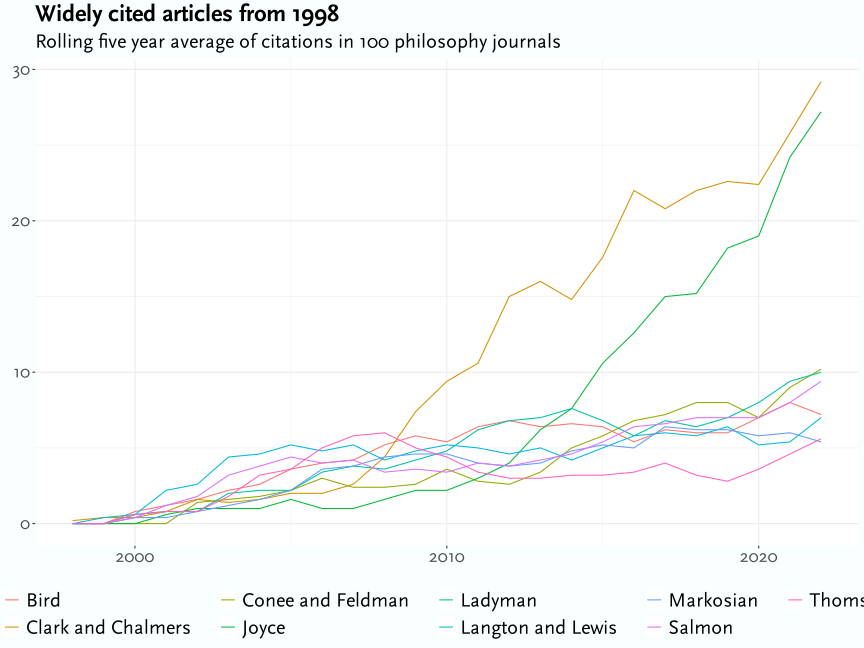
\includegraphics{citations_files/figure-pdf/fig-citation-spaghetti-1998-1.pdf}

}

\caption{\label{fig-citation-spaghetti-1998}Rolling five year average of
citation frequency for widely cited articles from 1998.}

\end{figure}%

\begin{figure}

\centering{

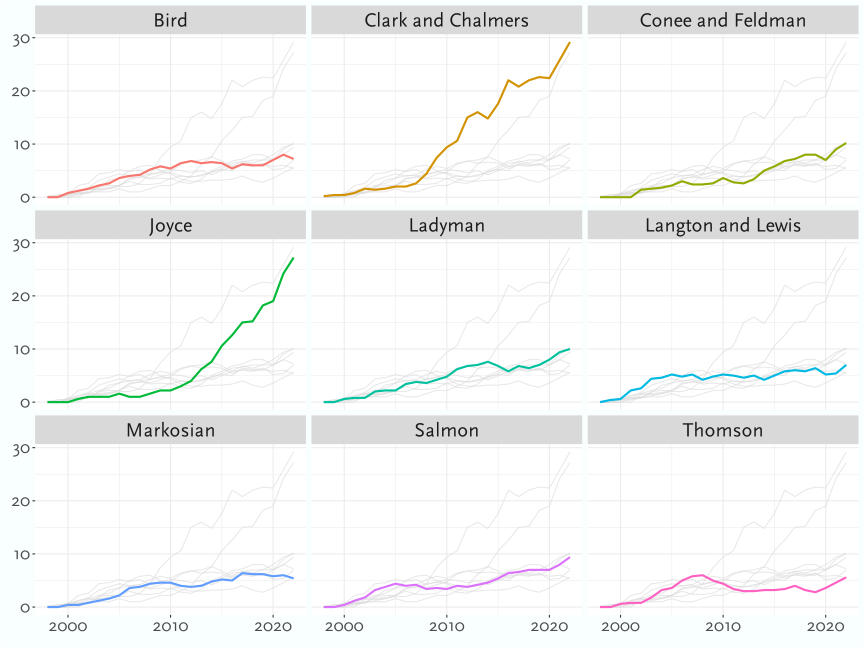
\includegraphics{citations_files/figure-pdf/fig-citation-facet-1998-1.pdf}

}

\caption{\label{fig-citation-facet-1998}Faceted version of
Figure~\ref{fig-citation-spaghetti-1998}.}

\end{figure}%

\newpage

\subsection{1999}\label{section-23}

\subsubsection*{Widely Cited Articles}\label{widely-cited-articles-23}
\addcontentsline{toc}{subsubsection}{Widely Cited Articles}

\begin{enumerate}
\def\labelenumi{\arabic{enumi}.}
\tightlist
\item
  ES Anderson, ``What is the Point of Equality?'' \emph{Ethics} 109 (2):
  287-337.
\item
  J Broome, ``Normative Requirements'' \emph{Ratio-New Series} 12 (4):
  398-419.
\item
  E Sosa, ``How To Defeat Opposition To Moore'' \emph{Noûs} 141-153.
\item
  N Block and R Stalnaker, ``Conceptual Analysis, Dualism, and the
  Explanatory Gap'' \emph{Philosophical Review} 108 (1): 1-46.
\item
  J Kim, ``Making Sense of Emergence'' \emph{Philosophical Studies} 95
  (1-2): 3-36.
\item
  JD Velleman, ``Love as a Moral Emotion'' \emph{Ethics} 109 (2):
  338-374.
\item
  S Cohen, ``Contextualism, Skepticism, and the Structure of Reasons''
  \emph{Noûs} 57-89.
\item
  J Hyman, ``How Knowledge Works'' \emph{Philosophical Quarterly} 49
  (197): 433-451.
\item
  T Shogenji, ``Is Coherence Truth Conducive?'' \emph{Analysis} 59 (4):
  338-345.
\end{enumerate}

\subsubsection*{Citation Count}\label{citation-count-23}
\addcontentsline{toc}{subsubsection}{Citation Count}

\begin{longtable}[]{@{}lrrr@{}}

\caption{\label{tbl-citation-count-1999}Citation count for widely cited
articles from 1999.}

\tabularnewline

\toprule\noalign{}
Article & All & Early & Late \\
\midrule\noalign{}
\endhead
\bottomrule\noalign{}
\endlastfoot
Anderson & 330 & 67 & 232 \\
Broome & 186 & 39 & 125 \\
Sosa & 170 & 0 & 165 \\
Block and Stalnaker & 151 & 57 & 70 \\
Kim & 124 & 45 & 52 \\
Velleman & 108 & 18 & 83 \\
Cohen & 102 & 0 & 94 \\
Shogenji & 93 & 36 & 45 \\
Hyman & 90 & 12 & 70 \\

\end{longtable}

\subsubsection*{Citation Rank}\label{citation-rank-23}
\addcontentsline{toc}{subsubsection}{Citation Rank}

\begin{longtable}[]{@{}lrrr@{}}

\caption{\label{tbl-citation-rank-1999}Citation rank for widely cited
articles from 1999.}

\tabularnewline

\toprule\noalign{}
Article & Overall & Early & Late \\
\midrule\noalign{}
\endhead
\bottomrule\noalign{}
\endlastfoot
Anderson & 1 & 1 & 1 \\
Broome & 2 & 4 & 3 \\
Sosa & 3 & 734 & 2 \\
Block and Stalnaker & 4 & 2 & 6 \\
Kim & 5 & 3 & 11 \\
Velleman & 6 & 18 & 5 \\
Cohen & 8 & 734 & 4 \\
Shogenji & 10 & 5 & 14 \\
Hyman & 11 & 35 & 6 \\

\end{longtable}

\subsubsection*{Citation Trends}\label{citation-trends-23}
\addcontentsline{toc}{subsubsection}{Citation Trends}

\begin{figure}

\centering{

\includegraphics{citations_files/figure-pdf/fig-citation-spaghetti-1999-1.pdf}

}

\caption{\label{fig-citation-spaghetti-1999}Rolling five year average of
citation frequency for widely cited articles from 1999.}

\end{figure}%

\begin{figure}

\centering{

\includegraphics{citations_files/figure-pdf/fig-citation-facet-1999-1.pdf}

}

\caption{\label{fig-citation-facet-1999}Faceted version of
Figure~\ref{fig-citation-spaghetti-1999}.}

\end{figure}%

\newpage

\subsection{2000}\label{section-24}

\subsubsection*{Widely Cited Articles}\label{widely-cited-articles-24}
\addcontentsline{toc}{subsubsection}{Widely Cited Articles}

\begin{enumerate}
\def\labelenumi{\arabic{enumi}.}
\tightlist
\item
  P Machamer, et al, ``Thinking About Mechanisms'' \emph{Philosophy Of
  Science} 67 (1): 1-25.
\item
  J Pryor, ``The Skeptic and the Dogmatist'' \emph{Noûs} 34 (4):
  517-549.
\item
  S Haslanger, ``Gender and Race: (What) Are They? (What) Do We Want
  Them To Be?'' \emph{Noûs} 34 (1): 31-55.
\item
  D Lewis, ``Causation as Influence'' \emph{Journal Of Philosophy} 97
  (4): 182-197.
\item
  J D'Arms and D Jacobson, ``The Moralistic Fallacy: On the
  `Appropriateness' of Emotions'' \emph{Philosophy And Phenomenological
  Research} 61 (1): 65-90.
\item
  H Douglas, ``Inductive Risk and Values in Science'' \emph{Philosophy
  Of Science} 67 (4): 559-579.
\item
  A Elga, ``Self-Locating Belief and the `Sleeping Beauty' Problem''
  \emph{Analysis} 60 (2): 143-147.
\item
  RG Heck, ``Nonconceptual Content and the''Space of Reasons''\,''
  \emph{Philosophical Review} 109 (4): 483-523.
\item
  LA Shapiro, ``Multiple Realizations'' \emph{Journal Of Philosophy} 97
  (12): 635-654.
\end{enumerate}

\subsubsection*{Citation Count}\label{citation-count-24}
\addcontentsline{toc}{subsubsection}{Citation Count}

\begin{longtable}[]{@{}lrrr@{}}

\caption{\label{tbl-citation-count-2000}Citation count for widely cited
articles from 2000.}

\tabularnewline

\toprule\noalign{}
Article & All & Early & Late \\
\midrule\noalign{}
\endhead
\bottomrule\noalign{}
\endlastfoot
Machamer et al & 494 & 100 & 347 \\
Pryor & 379 & 66 & 271 \\
Haslanger & 228 & 10 & 216 \\
Lewis & 212 & 63 & 135 \\
D'Arms and Jacobson & 197 & 27 & 156 \\
Douglas & 149 & 8 & 134 \\
Heck & 126 & 42 & 67 \\
Elga & 124 & 43 & 65 \\
Shapiro & 98 & 36 & 51 \\

\end{longtable}

\subsubsection*{Citation Rank}\label{citation-rank-24}
\addcontentsline{toc}{subsubsection}{Citation Rank}

\begin{longtable}[]{@{}lrrr@{}}

\caption{\label{tbl-citation-rank-2000}Citation rank for widely cited
articles from 2000.}

\tabularnewline

\toprule\noalign{}
Article & Overall & Early & Late \\
\midrule\noalign{}
\endhead
\bottomrule\noalign{}
\endlastfoot
Machamer et al & 1 & 1 & 1 \\
Pryor & 2 & 2 & 2 \\
Haslanger & 3 & 57 & 3 \\
Lewis & 4 & 3 & 5 \\
D'Arms and Jacobson & 5 & 8 & 4 \\
Douglas & 6 & 86 & 6 \\
Heck & 8 & 5 & 10 \\
Elga & 9 & 4 & 12 \\
Shapiro & 11 & 6 & 18 \\

\end{longtable}

\subsubsection*{Citation Trends}\label{citation-trends-24}
\addcontentsline{toc}{subsubsection}{Citation Trends}

\begin{figure}

\centering{

\includegraphics{citations_files/figure-pdf/fig-citation-spaghetti-2000-1.pdf}

}

\caption{\label{fig-citation-spaghetti-2000}Rolling five year average of
citation frequency for widely cited articles from 2000.}

\end{figure}%

\begin{figure}

\centering{

\includegraphics{citations_files/figure-pdf/fig-citation-facet-2000-1.pdf}

}

\caption{\label{fig-citation-facet-2000}Faceted version of
Figure~\ref{fig-citation-spaghetti-2000}.}

\end{figure}%

\newpage

\subsection{2001}\label{section-25}

\subsubsection*{Widely Cited Articles}\label{widely-cited-articles-25}
\addcontentsline{toc}{subsubsection}{Widely Cited Articles}

\begin{enumerate}
\def\labelenumi{\arabic{enumi}.}
\tightlist
\item
  J Stanley and T Williamson, ``Knowing How'' \emph{Journal Of
  Philosophy} 98 (8): 411-444.
\item
  DJ Chalmers and F Jackson, ``Conceptual Analysis and Reductive
  Explanation'' \emph{Philosophical Review} 110 (3): 315-360.
\item
  AI Goldman, ``Experts: Which Ones Should You Trust?'' \emph{Philosophy
  And Phenomenological Research} 63 (1): 85-110.
\item
  C Hitchcock, ``The Intransitivity of Causation Revealed in Equations
  and Graphs'' \emph{Journal Of Philosophy} 98 (6): 273-299.
\item
  P Rysiew, ``The Context-Sensitivity of Knowledge Attributions''
  \emph{Noûs} 35 (4): 477-514.
\item
  D Lewis, ``Truthmaking and Difference-Making'' \emph{Noûs} 35 (4):
  602-615.
\item
  CF Craver, ``Role Functions, Mechanisms, and Hierarchy''
  \emph{Philosophy Of Science} 68 (1): 53-74.
\item
  P Hieronymi, ``Articulating An Uncompromising Forgiveness''
  \emph{Philosophy And Phenomenological Research} 62 (3): 529-555.
\item
  C Peacocke, ``Does Perception Have a Nonconceptual Content?''
  \emph{Journal Of Philosophy} 98 (5): 239-264.
\end{enumerate}

\subsubsection*{Citation Count}\label{citation-count-25}
\addcontentsline{toc}{subsubsection}{Citation Count}

\begin{longtable}[]{@{}lrrr@{}}

\caption{\label{tbl-citation-count-2001}Citation count for widely cited
articles from 2001.}

\tabularnewline

\toprule\noalign{}
Article & All & Early & Late \\
\midrule\noalign{}
\endhead
\bottomrule\noalign{}
\endlastfoot
Stanley and Williamson & 261 & 65 & 188 \\
Chalmers and Jackson & 170 & 72 & 88 \\
Goldman & 135 & 14 & 118 \\
Hitchcock & 124 & 33 & 87 \\
Rysiew & 112 & 42 & 67 \\
Lewis & 101 & 29 & 68 \\
Craver & 94 & 37 & 54 \\
Peacocke & 92 & 46 & 43 \\
Hieronymi & 83 & 15 & 66 \\

\end{longtable}

\subsubsection*{Citation Rank}\label{citation-rank-25}
\addcontentsline{toc}{subsubsection}{Citation Rank}

\begin{longtable}[]{@{}lrrr@{}}

\caption{\label{tbl-citation-rank-2001}Citation rank for widely cited
articles from 2001.}

\tabularnewline

\toprule\noalign{}
Article & Overall & Early & Late \\
\midrule\noalign{}
\endhead
\bottomrule\noalign{}
\endlastfoot
Stanley and Williamson & 1 & 2 & 1 \\
Chalmers and Jackson & 2 & 1 & 3 \\
Goldman & 3 & 38 & 2 \\
Hitchcock & 4 & 6 & 4 \\
Rysiew & 5 & 4 & 6 \\
Lewis & 6 & 9 & 5 \\
Craver & 7 & 5 & 9 \\
Peacocke & 8 & 3 & 17 \\
Hieronymi & 10 & 31 & 7 \\

\end{longtable}

\subsubsection*{Citation Trends}\label{citation-trends-25}
\addcontentsline{toc}{subsubsection}{Citation Trends}

\begin{figure}

\centering{

\includegraphics{citations_files/figure-pdf/fig-citation-spaghetti-2001-1.pdf}

}

\caption{\label{fig-citation-spaghetti-2001}Rolling five year average of
citation frequency for widely cited articles from 2001.}

\end{figure}%

\begin{figure}

\centering{

\includegraphics{citations_files/figure-pdf/fig-citation-facet-2001-1.pdf}

}

\caption{\label{fig-citation-facet-2001}Faceted version of
Figure~\ref{fig-citation-spaghetti-2001}.}

\end{figure}%

\newpage

\subsection{2002}\label{section-26}

\subsubsection*{Widely Cited Articles}\label{widely-cited-articles-26}
\addcontentsline{toc}{subsubsection}{Widely Cited Articles}

\begin{enumerate}
\def\labelenumi{\arabic{enumi}.}
\tightlist
\item
  J Fantl and M McGrath, ``Evidence, Pragmatics, and Justification''
  \emph{Philosophical Review} 111 (1): 67-94.
\item
  S Cohen, ``Basic Knowledge and the Problem of Easy Knowledge''
  \emph{Philosophy And Phenomenological Research} 65 (2): 309-329.
\item
  S Glennan, ``Rethinking Mechanistic Explanation'' \emph{Philosophy Of
  Science} 69 (3): 342-353.
\item
  R Chang, ``The Possibility of Parity'' \emph{Ethics} 112 (4): 659-688.
\item
  R Wedgwood, ``The Aim of Belief'' \emph{Noûs} 267-297.
\item
  C Wright, ``(Anti-)Sceptics Simple and Subtle: G.E. Moore and John
  McDowell'' \emph{Philosophy And Phenomenological Research} 65 (2):
  330-348.
\item
  E Schwitzgebel, ``A Phenomenal, Dispositional Account of Belief''
  \emph{Noûs} 36 (2): 249-275.
\item
  M Matthen and A Ariew, ``Two Ways of Thinking About Fitness and
  Natural Selection'' \emph{Journal Of Philosophy} 99 (2): 55-83.
\item
  DM Walsh, et al, ``The Trials of Life: Natural Selection and Random
  Drift'' \emph{Philosophy Of Science} 69 (3): 452-473.
\end{enumerate}

\subsubsection*{Citation Count}\label{citation-count-26}
\addcontentsline{toc}{subsubsection}{Citation Count}

\begin{longtable}[]{@{}lrrr@{}}

\caption{\label{tbl-citation-count-2002}Citation count for widely cited
articles from 2002.}

\tabularnewline

\toprule\noalign{}
Article & All & Early & Late \\
\midrule\noalign{}
\endhead
\bottomrule\noalign{}
\endlastfoot
Fantl and McGrath & 205 & 48 & 157 \\
Cohen & 151 & 49 & 102 \\
Glennan & 151 & 58 & 93 \\
Chang & 142 & 29 & 113 \\
Wedgwood & 136 & 7 & 129 \\
Wright & 117 & 48 & 69 \\
Schwitzgebel & 96 & 18 & 78 \\
Matthen and Ariew & 95 & 46 & 49 \\
Walsh et al & 88 & 39 & 49 \\

\end{longtable}

\subsubsection*{Citation Rank}\label{citation-rank-26}
\addcontentsline{toc}{subsubsection}{Citation Rank}

\begin{longtable}[]{@{}lrrr@{}}

\caption{\label{tbl-citation-rank-2002}Citation rank for widely cited
articles from 2002.}

\tabularnewline

\toprule\noalign{}
Article & Overall & Early & Late \\
\midrule\noalign{}
\endhead
\bottomrule\noalign{}
\endlastfoot
Fantl and McGrath & 1 & 3 & 1 \\
Cohen & 2 & 2 & 4 \\
Glennan & 2 & 1 & 5 \\
Chang & 4 & 10 & 3 \\
Wedgwood & 5 & 121 & 2 \\
Wright & 6 & 3 & 7 \\
Schwitzgebel & 7 & 26 & 6 \\
Matthen and Ariew & 8 & 5 & 12 \\
Walsh et al & 10 & 6 & 12 \\

\end{longtable}

\subsubsection*{Citation Trends}\label{citation-trends-26}
\addcontentsline{toc}{subsubsection}{Citation Trends}

\begin{figure}

\centering{

\includegraphics{citations_files/figure-pdf/fig-citation-spaghetti-2002-1.pdf}

}

\caption{\label{fig-citation-spaghetti-2002}Rolling five year average of
citation frequency for widely cited articles from 2002.}

\end{figure}%

\begin{figure}

\centering{

\includegraphics{citations_files/figure-pdf/fig-citation-facet-2002-1.pdf}

}

\caption{\label{fig-citation-facet-2002}Faceted version of
Figure~\ref{fig-citation-spaghetti-2002}.}

\end{figure}%

\newpage

\subsection{2003}\label{section-27}

\subsubsection*{Widely Cited Articles}\label{widely-cited-articles-27}
\addcontentsline{toc}{subsubsection}{Widely Cited Articles}

\begin{enumerate}
\def\labelenumi{\arabic{enumi}.}
\tightlist
\item
  K DeRose, ``Assertion, Knowledge, and Context'' \emph{Philosophical
  Review} 111 (2): 167-203.
\item
  N Shah, ``How Truth Governs Belief'' \emph{Philosophical Review} 112
  (4): 447-482.
\item
  J Knobe, ``Intentional Action and Side Effects in Ordinary Language''
  \emph{Analysis} 63 (3): 190-194.
\item
  A Hájek, ``What Conditional Probability Could Not Be'' \emph{Synthese}
  137 (3): 273-323.
\item
  T Burge, ``Perceptual Entitlement'' \emph{Philosophy And
  Phenomenological Research} 67 (3): 503-548.
\item
  T Kelly, ``Epistemic Rationality as Instrumental Rationality: A
  Critique'' \emph{Philosophy And Phenomenological Research} 66 (3):
  612-640.
\item
  J Schaffer, ``Is There a Fundamental Level?'' \emph{Noûs} 37 (3):
  498-517.
\item
  N Kolodny, ``Love as Valuing a Relationship'' \emph{Philosophical
  Review} 112 (2): 135-189.
\item
  J MacFarlane, ``Future Contingents and Relative Truth''
  \emph{Philosophical Quarterly} 53 (212): 321-336.
\end{enumerate}

\subsubsection*{Citation Count}\label{citation-count-27}
\addcontentsline{toc}{subsubsection}{Citation Count}

\begin{longtable}[]{@{}lrrr@{}}

\caption{\label{tbl-citation-count-2003}Citation count for widely cited
articles from 2003.}

\tabularnewline

\toprule\noalign{}
Article & All & Early & Late \\
\midrule\noalign{}
\endhead
\bottomrule\noalign{}
\endlastfoot
Derose & 207 & 85 & 137 \\
Shah & 159 & 48 & 119 \\
Knobe & 150 & 73 & 92 \\
Hájek & 147 & 47 & 107 \\
Burge & 134 & 50 & 93 \\
Kelly & 131 & 32 & 109 \\
Schaffer & 115 & 45 & 75 \\
MacFarlane & 107 & 51 & 64 \\
Kolodny & 104 & 22 & 88 \\

\end{longtable}

\subsubsection*{Citation Rank}\label{citation-rank-27}
\addcontentsline{toc}{subsubsection}{Citation Rank}

\begin{longtable}[]{@{}lrrr@{}}

\caption{\label{tbl-citation-rank-2003}Citation rank for widely cited
articles from 2003.}

\tabularnewline

\toprule\noalign{}
Article & Overall & Early & Late \\
\midrule\noalign{}
\endhead
\bottomrule\noalign{}
\endlastfoot
Derose & 1 & 1 & 1 \\
Shah & 2 & 5 & 2 \\
Knobe & 3 & 2 & 6 \\
Hájek & 4 & 7 & 4 \\
Burge & 5 & 4 & 5 \\
Kelly & 6 & 15 & 3 \\
Schaffer & 7 & 8 & 9 \\
MacFarlane & 8 & 3 & 12 \\
Kolodny & 9 & 26 & 7 \\

\end{longtable}

\subsubsection*{Citation Trends}\label{citation-trends-27}
\addcontentsline{toc}{subsubsection}{Citation Trends}

\begin{figure}

\centering{

\includegraphics{citations_files/figure-pdf/fig-citation-spaghetti-2003-1.pdf}

}

\caption{\label{fig-citation-spaghetti-2003}Rolling five year average of
citation frequency for widely cited articles from 2003.}

\end{figure}%

\begin{figure}

\centering{

\includegraphics{citations_files/figure-pdf/fig-citation-facet-2003-1.pdf}

}

\caption{\label{fig-citation-facet-2003}Faceted version of
Figure~\ref{fig-citation-spaghetti-2003}.}

\end{figure}%

\newpage

\subsection{2004}\label{section-28}

\subsubsection*{Widely Cited Articles}\label{widely-cited-articles-28}
\addcontentsline{toc}{subsubsection}{Widely Cited Articles}

\begin{enumerate}
\def\labelenumi{\arabic{enumi}.}
\tightlist
\item
  W Rabinowicz and T Ronnow-Rasmussen, ``The Strike of the Demon: On
  Fitting Pro-Attitudes and Value'' \emph{Ethics} 114 (3): 391-423.
\item
  MGF Martin, ``The Limits of Self-Awareness'' \emph{Philosophical
  Studies} 120 (1-3): 37-89 -.
\item
  C Travis, ``The Silence of the Senses'' \emph{Mind} 113 (449): 57-94.
\item
  J Pryor, ``What's Wrong With Moore's Argument?'' \emph{Noûs} 349-378
  14.
\item
  D Pitt, ``The Phenomenology of Cognition, Or, What is It Like To Think
  That P?'' \emph{Philosophy And Phenomenological Research} 69 (1):
  1-36.
\item
  M Johnston, ``The Obscure Object of Hallucination''
  \emph{Philosophical Studies} 120 (1-3): 113-183 -.
\item
  RN Giere, ``How Models Are Used To Represent Reality''
  \emph{Philosophy Of Science} 71 (5): 742-752.
\item
  M Richard, ``Contextualism and Relativism'' \emph{Philosophical
  Studies} 119 (1-2): 215-242.
\item
  J Schaffer, ``From Contextualism To Contrastivism''
  \emph{Philosophical Studies} 119 (1-2): 73-103.
\end{enumerate}

\subsubsection*{Citation Count}\label{citation-count-28}
\addcontentsline{toc}{subsubsection}{Citation Count}

\begin{longtable}[]{@{}lrrr@{}}

\caption{\label{tbl-citation-count-2004}Citation count for widely cited
articles from 2004.}

\tabularnewline

\toprule\noalign{}
Article & All & Early & Late \\
\midrule\noalign{}
\endhead
\bottomrule\noalign{}
\endlastfoot
R and R-R & 175 & 79 & 115 \\
Martin & 171 & 56 & 129 \\
Travis & 170 & 69 & 118 \\
Pryor & 131 & 26 & 125 \\
Pitt & 126 & 55 & 87 \\
Johnston & 114 & 40 & 89 \\
Giere & 106 & 34 & 83 \\
Richard & 71 & 44 & 40 \\
Schaffer & 67 & 42 & 38 \\

\end{longtable}

\subsubsection*{Citation Rank}\label{citation-rank-28}
\addcontentsline{toc}{subsubsection}{Citation Rank}

\begin{longtable}[]{@{}lrrr@{}}

\caption{\label{tbl-citation-rank-2004}Citation rank for widely cited
articles from 2004.}

\tabularnewline

\toprule\noalign{}
Article & Overall & Early & Late \\
\midrule\noalign{}
\endhead
\bottomrule\noalign{}
\endlastfoot
R and R-R & 1 & 1 & 4 \\
Martin & 2 & 3 & 1 \\
Travis & 3 & 2 & 3 \\
Pryor & 4 & 20 & 2 \\
Pitt & 5 & 4 & 6 \\
Johnston & 6 & 8 & 5 \\
Giere & 7 & 11 & 7 \\
Richard & 13 & 5 & 24 \\
Schaffer & 16 & 6 & 25 \\

\end{longtable}

\subsubsection*{Citation Trends}\label{citation-trends-28}
\addcontentsline{toc}{subsubsection}{Citation Trends}

\begin{figure}

\centering{

\includegraphics{citations_files/figure-pdf/fig-citation-spaghetti-2004-1.pdf}

}

\caption{\label{fig-citation-spaghetti-2004}Rolling five year average of
citation frequency for widely cited articles from 2004.}

\end{figure}%

\begin{figure}

\centering{

\includegraphics{citations_files/figure-pdf/fig-citation-facet-2004-1.pdf}

}

\caption{\label{fig-citation-facet-2004}Faceted version of
Figure~\ref{fig-citation-spaghetti-2004}.}

\end{figure}%

\newpage

\subsection{2005}\label{section-29}

\subsubsection*{Widely Cited Articles}\label{widely-cited-articles-29}
\addcontentsline{toc}{subsubsection}{Widely Cited Articles}

\begin{enumerate}
\def\labelenumi{\arabic{enumi}.}
\tightlist
\item
  N Kolodny, ``Why Be Rational?'' \emph{Mind} 114 (455): 509-563.
\item
  Nishi Shah and J. David Velleman, ``Doxastic Deliberation''
  \emph{Philosophical Review} 114 (4): 497-534.
\item
  AM Smith, ``Responsibility for Attitudes: Activity and Passivity in
  Mental Life'' \emph{Ethics} 115 (2): 236-271.
\item
  P Hieronymi, ``The Wrong Kind of Reason'' \emph{Journal Of Philosophy}
  102 (9): 437-457.
\item
  A Baker, ``Are There Genuine Mathematical Explanations of Physical
  Phenomena?'' \emph{Mind} 114 (454): 223-238.
\item
  Matthew Weiner, ``Must We Know What We Say?'' \emph{Philosophical
  Review} 114 (2): 227-251.
\item
  T Williamson, ``Contextualism, Subject-Sensitive Invariantism and
  Knowledge of Knowledge'' \emph{Philosophical Quarterly} 55 (219):
  213-235.
\item
  Jonathan Schaffer, ``Contrastive Causation'' \emph{Philosophical
  Review} 114 (3): 327-358.
\item
  E Nahmias, et al, ``Surveying Freedom: Folk Intuitions About Free Will
  and Moral Responsibility'' \emph{Philosophical Psychology} 18 (5):
  561-584.
\end{enumerate}

\subsubsection*{Citation Count}\label{citation-count-29}
\addcontentsline{toc}{subsubsection}{Citation Count}

\begin{longtable}[]{@{}lrrr@{}}

\caption{\label{tbl-citation-count-2005}Citation count for widely cited
articles from 2005.}

\tabularnewline

\toprule\noalign{}
Article & All & Early & Late \\
\midrule\noalign{}
\endhead
\bottomrule\noalign{}
\endlastfoot
Kolodny & 251 & 95 & 203 \\
Shah and Velleman & 213 & 62 & 177 \\
Smith & 169 & 51 & 151 \\
Hieronymi & 153 & 39 & 126 \\
Baker & 131 & 39 & 107 \\
Weiner & 129 & 67 & 96 \\
Williamson & 109 & 48 & 85 \\
Schaffer & 105 & 44 & 85 \\
Nahmias et al & 62 & 41 & 38 \\

\end{longtable}

\subsubsection*{Citation Rank}\label{citation-rank-29}
\addcontentsline{toc}{subsubsection}{Citation Rank}

\begin{longtable}[]{@{}lrrr@{}}

\caption{\label{tbl-citation-rank-2005}Citation rank for widely cited
articles from 2005.}

\tabularnewline

\toprule\noalign{}
Article & Overall & Early & Late \\
\midrule\noalign{}
\endhead
\bottomrule\noalign{}
\endlastfoot
Kolodny & 1 & 1 & 1 \\
Shah and Velleman & 2 & 3 & 2 \\
Smith & 3 & 4 & 3 \\
Hieronymi & 4 & 10 & 4 \\
Baker & 5 & 10 & 5 \\
Weiner & 6 & 2 & 6 \\
Williamson & 7 & 5 & 7 \\
Schaffer & 8 & 6 & 7 \\
Nahmias et al & 19 & 7 & 31 \\

\end{longtable}

\subsubsection*{Citation Trends}\label{citation-trends-29}
\addcontentsline{toc}{subsubsection}{Citation Trends}

\begin{figure}

\centering{

\includegraphics{citations_files/figure-pdf/fig-citation-spaghetti-2005-1.pdf}

}

\caption{\label{fig-citation-spaghetti-2005}Rolling five year average of
citation frequency for widely cited articles from 2005.}

\end{figure}%

\begin{figure}

\centering{

\includegraphics{citations_files/figure-pdf/fig-citation-facet-2005-1.pdf}

}

\caption{\label{fig-citation-facet-2005}Faceted version of
Figure~\ref{fig-citation-spaghetti-2005}.}

\end{figure}%

\newpage

\subsection{2006}\label{section-30}

\subsubsection*{Widely Cited Articles}\label{widely-cited-articles-30}
\addcontentsline{toc}{subsubsection}{Widely Cited Articles}

\begin{enumerate}
\def\labelenumi{\arabic{enumi}.}
\tightlist
\item
  S Street, ``A Darwinian Dilemma for Realist Theories of Value''
  \emph{Philosophical Studies} 27 (1): 109-166.
\item
  Hilary Greaves and David Wallace, ``Justifying Conditionalization:
  Conditionalization Maximizes Expected Epistemic Utility'' \emph{Mind}
  115 (459): 607-632.
\item
  Igor Douven, ``Assertion, Knowledge, and Rational Credibility''
  \emph{Philosophical Review} 115 (4): 449-485.
\item
  Peter Godfrey-Smith, ``The Strategy of Model-Based Science''
  \emph{Biology \& Philosophy} 21 (5): 725-740.
\item
  Roger White, ``Problems for Dogmatism'' \emph{Philosophical Studies}
  131 (3): 525-557.
\item
  David Enoch, ``Agency, Shmagency: Why Normativity Won't Come From What
  is Constitutive of Action'' \emph{Philosophical Review} 115 (2):
  169-198.
\item
  Nishi Shah, ``A New Argument for Evidentialism'' \emph{Philosophical
  Quarterly} 56 (225): 481-498.
\item
  Carl F. Craver, ``When Mechanistic Models Explain'' \emph{Synthese}
  153 (3): 355-376.
\item
  Bill Brewer, ``Perception and Content'' \emph{European Journal Of
  Philosophy} 14 (2): 165-181.
\end{enumerate}

\subsubsection*{Citation Count}\label{citation-count-30}
\addcontentsline{toc}{subsubsection}{Citation Count}

\begin{longtable}[]{@{}lrrr@{}}

\caption{\label{tbl-citation-count-2006}Citation count for widely cited
articles from 2006.}

\tabularnewline

\toprule\noalign{}
Article & All & Early & Late \\
\midrule\noalign{}
\endhead
\bottomrule\noalign{}
\endlastfoot
Street & 275 & 92 & 246 \\
Greaves and Wallace & 135 & 35 & 126 \\
Douven & 121 & 62 & 98 \\
Godfrey-Smith & 119 & 55 & 88 \\
White & 118 & 71 & 88 \\
Craver & 115 & 48 & 94 \\
Enoch & 111 & 47 & 98 \\
Shah & 107 & 36 & 94 \\
Brewer & 91 & 50 & 67 \\

\end{longtable}

\subsubsection*{Citation Rank}\label{citation-rank-30}
\addcontentsline{toc}{subsubsection}{Citation Rank}

\begin{longtable}[]{@{}lrrr@{}}

\caption{\label{tbl-citation-rank-2006}Citation rank for widely cited
articles from 2006.}

\tabularnewline

\toprule\noalign{}
Article & Overall & Early & Late \\
\midrule\noalign{}
\endhead
\bottomrule\noalign{}
\endlastfoot
Street & 1 & 1 & 1 \\
Greaves and Wallace & 2 & 16 & 2 \\
Douven & 3 & 3 & 3 \\
Godfrey-Smith & 4 & 4 & 8 \\
White & 5 & 2 & 8 \\
Craver & 6 & 6 & 5 \\
Enoch & 8 & 7 & 3 \\
Shah & 9 & 14 & 5 \\
Brewer & 11 & 5 & 13 \\

\end{longtable}

\subsubsection*{Citation Trends}\label{citation-trends-30}
\addcontentsline{toc}{subsubsection}{Citation Trends}

\begin{figure}

\centering{

\includegraphics{citations_files/figure-pdf/fig-citation-spaghetti-2006-1.pdf}

}

\caption{\label{fig-citation-spaghetti-2006}Rolling five year average of
citation frequency for widely cited articles from 2006.}

\end{figure}%

\begin{figure}

\centering{

\includegraphics{citations_files/figure-pdf/fig-citation-facet-2006-1.pdf}

}

\caption{\label{fig-citation-facet-2006}Faceted version of
Figure~\ref{fig-citation-spaghetti-2006}.}

\end{figure}%

\newpage

\subsection{2007}\label{section-31}

\subsubsection*{Widely Cited Articles}\label{widely-cited-articles-31}
\addcontentsline{toc}{subsubsection}{Widely Cited Articles}

\begin{enumerate}
\def\labelenumi{\arabic{enumi}.}
\tightlist
\item
  Adam Elga, ``Reflection and Disagreement'' \emph{Noûs} 41 (3):
  478-502.
\item
  David Christensen, ``Epistemology of Disagreement: The Good News''
  \emph{Philosophical Review} 116 (2): 187-217.
\item
  Jennifer Lackey, ``Norms of Assertion'' \emph{Noûs} 41 (4): 594-626.
\item
  Seth Yalcin, ``Epistemic Modals'' \emph{Mind} 116 (464): 983-1026.
\item
  Michael Huemer, ``Compassionate Phenomenal Conservatism''
  \emph{Philosophy And Phenomenological Research} 74 (1): 30-55.
\item
  Michael Weisberg, ``Three Kinds of Idealization'' \emph{Journal Of
  Philosophy} 104 (12): 639-659.
\item
  Duncan Pritchard, ``Anti-Luck Epistemology'' \emph{Synthese} 158 (3):
  277-297.
\item
  John MacFarlane, ``Relativism and Disagreement'' \emph{Philosophical
  Studies} 132 (1): 17-31.
\item
  Andy Egan, ``Epistemic Modals, Relativism and Assertion''
  \emph{Philosophical Studies} 133 (1): 1-22.
\end{enumerate}

\subsubsection*{Citation Count}\label{citation-count-31}
\addcontentsline{toc}{subsubsection}{Citation Count}

\begin{longtable}[]{@{}lrrr@{}}

\caption{\label{tbl-citation-count-2007}Citation count for widely cited
articles from 2007.}

\tabularnewline

\toprule\noalign{}
Article & All & Early & Late \\
\midrule\noalign{}
\endhead
\bottomrule\noalign{}
\endlastfoot
Elga & 282 & 144 & 238 \\
Christensen & 275 & 140 & 232 \\
Lackey & 173 & 96 & 147 \\
Yalcin & 166 & 68 & 157 \\
Huemer & 142 & 76 & 122 \\
Weisberg & 136 & 63 & 121 \\
Pritchard & 115 & 63 & 96 \\
Egan & 111 & 71 & 83 \\
MacFarlane & 110 & 74 & 79 \\

\end{longtable}

\subsubsection*{Citation Rank}\label{citation-rank-31}
\addcontentsline{toc}{subsubsection}{Citation Rank}

\begin{longtable}[]{@{}lrrr@{}}

\caption{\label{tbl-citation-rank-2007}Citation rank for widely cited
articles from 2007.}

\tabularnewline

\toprule\noalign{}
Article & Overall & Early & Late \\
\midrule\noalign{}
\endhead
\bottomrule\noalign{}
\endlastfoot
Elga & 1 & 1 & 1 \\
Christensen & 2 & 2 & 2 \\
Lackey & 3 & 3 & 4 \\
Yalcin & 4 & 7 & 3 \\
Huemer & 5 & 4 & 5 \\
Weisberg & 6 & 9 & 6 \\
Pritchard & 7 & 9 & 7 \\
Egan & 8 & 6 & 8 \\
MacFarlane & 9 & 5 & 9 \\

\end{longtable}

\subsubsection*{Citation Trends}\label{citation-trends-31}
\addcontentsline{toc}{subsubsection}{Citation Trends}

\begin{figure}

\centering{

\includegraphics{citations_files/figure-pdf/fig-citation-spaghetti-2007-1.pdf}

}

\caption{\label{fig-citation-spaghetti-2007}Rolling five year average of
citation frequency for widely cited articles from 2007.}

\end{figure}%

\begin{figure}

\centering{

\includegraphics{citations_files/figure-pdf/fig-citation-facet-2007-1.pdf}

}

\caption{\label{fig-citation-facet-2007}Faceted version of
Figure~\ref{fig-citation-spaghetti-2007}.}

\end{figure}%

\newpage

\subsection{2008}\label{section-32}

\subsubsection*{Widely Cited Articles}\label{widely-cited-articles-32}
\addcontentsline{toc}{subsubsection}{Widely Cited Articles}

\begin{enumerate}
\def\labelenumi{\arabic{enumi}.}
\tightlist
\item
  John Hawthorne and Jason Stanley, ``Knowledge and Action''
  \emph{Journal Of Philosophy} 5 (10): 571-590.
\item
  Tamar Szabo Gendler, ``Alief and Belief'' \emph{Journal Of Philosophy}
  5 (10): 634-663.
\item
  Eric Schwitzgebel, ``The Unreliability of Naive Introspection''
  \emph{Philosophical Review} 117 (2): 245-273.
\item
  Jessica Brown, ``Subject-Sensitive Invariantism and the Knowledge Norm
  for Practical Reasoning'' \emph{Noûs} 42 (2): 167-189.
\item
  Stacey Swain, et al, ``The Instability of Philosophical Intuitions:
  Running Hot and Cold on Truetemp'' \emph{Philosophy And
  Phenomenological Research} 76 (1): 138-155.
\item
  Scott Sturgeon, ``Reason and the Grain of Belief'' \emph{Noûs} 42 (1):
  139-165.
\item
  Michael Fara, ``Masked Abilities and Compatibilism'' \emph{Mind} 117
  (468): 843-865.
\item
  Pamela Hieronymi, ``Responsibility for Believing'' \emph{Synthese} 161
  (3): 357-373.
\item
  Ross P. Cameron, ``Turtles All the Way Down: Regress, Priority and
  Fundamentality'' \emph{Philosophical Quarterly} 58 (230): 1-14.
\end{enumerate}

\subsubsection*{Citation Count}\label{citation-count-32}
\addcontentsline{toc}{subsubsection}{Citation Count}

\begin{longtable}[]{@{}lrrr@{}}

\caption{\label{tbl-citation-count-2008}Citation count for widely cited
articles from 2008.}

\tabularnewline

\toprule\noalign{}
Article & All & Early & Late \\
\midrule\noalign{}
\endhead
\bottomrule\noalign{}
\endlastfoot
Hawthorne and Stanley & 251 & 137 & 219 \\
Gendler & 170 & 100 & 156 \\
Schwitzgebel & 107 & 59 & 92 \\
Brown & 98 & 46 & 87 \\
Swain et al & 97 & 74 & 67 \\
Sturgeon & 97 & 43 & 92 \\
Fara & 94 & 60 & 83 \\
Hieronymi & 87 & 43 & 79 \\
Cameron & 86 & 56 & 77 \\

\end{longtable}

\subsubsection*{Citation Rank}\label{citation-rank-32}
\addcontentsline{toc}{subsubsection}{Citation Rank}

\begin{longtable}[]{@{}lrrr@{}}

\caption{\label{tbl-citation-rank-2008}Citation rank for widely cited
articles from 2008.}

\tabularnewline

\toprule\noalign{}
Article & Overall & Early & Late \\
\midrule\noalign{}
\endhead
\bottomrule\noalign{}
\endlastfoot
Hawthorne and Stanley & 1 & 1 & 1 \\
Gendler & 2 & 2 & 2 \\
Schwitzgebel & 3 & 5 & 3 \\
Brown & 4 & 8 & 5 \\
Swain et al & 5 & 3 & 10 \\
Sturgeon & 5 & 11 & 3 \\
Fara & 7 & 4 & 6 \\
Hieronymi & 8 & 11 & 7 \\
Cameron & 9 & 6 & 8 \\

\end{longtable}

\subsubsection*{Citation Trends}\label{citation-trends-32}
\addcontentsline{toc}{subsubsection}{Citation Trends}

\begin{figure}

\centering{

\includegraphics{citations_files/figure-pdf/fig-citation-spaghetti-2008-1.pdf}

}

\caption{\label{fig-citation-spaghetti-2008}Rolling five year average of
citation frequency for widely cited articles from 2008.}

\end{figure}%

\begin{figure}

\centering{

\includegraphics{citations_files/figure-pdf/fig-citation-facet-2008-1.pdf}

}

\caption{\label{fig-citation-facet-2008}Faceted version of
Figure~\ref{fig-citation-spaghetti-2008}.}

\end{figure}%

\newpage

\subsection{2009}\label{section-33}

\subsubsection*{Widely Cited Articles}\label{widely-cited-articles-33}
\addcontentsline{toc}{subsubsection}{Widely Cited Articles}

\begin{enumerate}
\def\labelenumi{\arabic{enumi}.}
\tightlist
\item
  Alison Hills, ``Moral Testimony and Moral Epistemology'' \emph{Ethics}
  120 (1): 94-127.
\item
  Alan Baker, ``Mathematical Explanation in Science'' \emph{British
  Journal For The Philosophy Of Science} 60 (3): 611-633.
\item
  John MacFarlane, ``Nonindexical Contextualism'' \emph{Synthese} 166
  (2): 231-250.
\item
  Alex Byrne, ``Experience and Content'' \emph{Philosophical Quarterly}
  59 (236): 429-451.
\item
  Jonathan Schaffer, ``Spacetime the One Substance'' \emph{Philosophical
  Studies} 145 (1): 131-148.
\item
  Jonathan Cohen and Craig Callender, ``A Better Best System Account of
  Lawhood'' \emph{Philosophical Studies} 145 (1): 1-34.
\item
  Christian List and Peter Menzies, ``Nonreductive Physicalism and the
  Limits of the Exclusion Principle'' \emph{Journal Of Philosophy} 106
  (9): 475-502.
\item
  Mark Schroeder, ``Means-End Coherence, Stringency, and Subjective
  Reasons'' \emph{Philosophical Studies} 143 (2): 223-248.
\item
  Jonathan Quong, ``Killing in Self-Defense'' \emph{Ethics} 119 (3):
  507-537.
\end{enumerate}

\subsubsection*{Citation Count}\label{citation-count-33}
\addcontentsline{toc}{subsubsection}{Citation Count}

\begin{longtable}[]{@{}lrrr@{}}

\caption{\label{tbl-citation-count-2009}Citation count for widely cited
articles from 2009.}

\tabularnewline

\toprule\noalign{}
Article & All & Early & Late \\
\midrule\noalign{}
\endhead
\bottomrule\noalign{}
\endlastfoot
Hills & 127 & 60 & 124 \\
Baker & 89 & 53 & 81 \\
MacFarlane & 83 & 67 & 62 \\
Byrne & 83 & 58 & 73 \\
Schaffer & 79 & 45 & 70 \\
Cohen and Callender & 77 & 41 & 74 \\
Schroeder & 76 & 51 & 62 \\
List and Menzies & 76 & 47 & 71 \\
Quong & 55 & 47 & 42 \\

\end{longtable}

\subsubsection*{Citation Rank}\label{citation-rank-33}
\addcontentsline{toc}{subsubsection}{Citation Rank}

\begin{longtable}[]{@{}lrrr@{}}

\caption{\label{tbl-citation-rank-2009}Citation rank for widely cited
articles from 2009.}

\tabularnewline

\toprule\noalign{}
Article & Overall & Early & Late \\
\midrule\noalign{}
\endhead
\bottomrule\noalign{}
\endlastfoot
Hills & 1 & 2 & 1 \\
Baker & 2 & 4 & 2 \\
MacFarlane & 3 & 1 & 9 \\
Byrne & 3 & 3 & 4 \\
Schaffer & 5 & 9 & 6 \\
Cohen and Callender & 6 & 11 & 3 \\
Schroeder & 7 & 5 & 9 \\
List and Menzies & 7 & 6 & 5 \\
Quong & 18 & 6 & 29 \\

\end{longtable}

\subsubsection*{Citation Trends}\label{citation-trends-33}
\addcontentsline{toc}{subsubsection}{Citation Trends}

\begin{figure}

\centering{

\includegraphics{citations_files/figure-pdf/fig-citation-spaghetti-2009-1.pdf}

}

\caption{\label{fig-citation-spaghetti-2009}Rolling five year average of
citation frequency for widely cited articles from 2009.}

\end{figure}%

\begin{figure}

\centering{

\includegraphics{citations_files/figure-pdf/fig-citation-facet-2009-1.pdf}

}

\caption{\label{fig-citation-facet-2009}Faceted version of
Figure~\ref{fig-citation-spaghetti-2009}.}

\end{figure}%

\newpage

\subsection{2010}\label{section-34}

\subsubsection*{Widely Cited Articles}\label{widely-cited-articles-34}
\addcontentsline{toc}{subsubsection}{Widely Cited Articles}

\begin{enumerate}
\def\labelenumi{\arabic{enumi}.}
\tightlist
\item
  David Christensen, ``Higher-Order Evidence'' \emph{Philosophy And
  Phenomenological Research} 81 (1): 185-215.
\item
  Niko Kolodny and John MacFarlane, ``Ifs and Oughts'' \emph{Journal Of
  Philosophy} 107 (3): 115-143.
\item
  James Woodward, ``Causation in Biology: Stability, Specificity, and
  the Choice of Levels of Explanation'' \emph{Biology \& Philosophy} 25
  (3): 287-318.
\item
  Maria Lasonen Aarnio, ``Unreasonable Knowledge'' \emph{Philosophical
  Perspectives} 24 (1): 1-21.
\item
  Eric Schwitzgebel, ``Acting Contrary To Our Professed Beliefs or the
  Gulf Between Occurrent Judgment and Dispositional Belief''
  \emph{Pacific Philosophical Quarterly} 91 (4): 531-553.
\item
  Julia Markovits, ``Acting for the Right Reasons'' \emph{Philosophical
  Review} 119 (2): 201-242.
\item
  Jonathan Schaffer, ``The Least Discerning and Most Promiscuous
  Truthmaker'' \emph{Philosophical Quarterly} 60 (239): 307-324.
\item
  Kevin J. S. Zollman, ``The Epistemic Benefit of Transient Diversity''
  \emph{Erkenntnis} 72 (1): 17-35.
\item
  John Turri, ``On the Relationship Between Propositional and Doxastic
  Justification'' \emph{Philosophy And Phenomenological Research} 80
  (2): 312-326.
\end{enumerate}

\subsubsection*{Citation Count}\label{citation-count-34}
\addcontentsline{toc}{subsubsection}{Citation Count}

\begin{longtable}[]{@{}lrrr@{}}

\caption{\label{tbl-citation-count-2010}Citation count for widely cited
articles from 2010.}

\tabularnewline

\toprule\noalign{}
Article & All & Early & Late \\
\midrule\noalign{}
\endhead
\bottomrule\noalign{}
\endlastfoot
Christensen & 140 & 84 & 132 \\
Kolodny and MacFarlane & 123 & 89 & 117 \\
Woodward & 120 & 89 & 115 \\
Aarnio & 101 & 55 & 100 \\
Schwitzgebel & 98 & 72 & 94 \\
Markovits & 96 & 62 & 93 \\
Schaffer & 95 & 75 & 89 \\
Zollman & 92 & 54 & 89 \\
Turri & 90 & 72 & 83 \\

\end{longtable}

\subsubsection*{Citation Rank}\label{citation-rank-34}
\addcontentsline{toc}{subsubsection}{Citation Rank}

\begin{longtable}[]{@{}lrrr@{}}

\caption{\label{tbl-citation-rank-2010}Citation rank for widely cited
articles from 2010.}

\tabularnewline

\toprule\noalign{}
Article & Overall & Early & Late \\
\midrule\noalign{}
\endhead
\bottomrule\noalign{}
\endlastfoot
Christensen & 1 & 3 & 1 \\
Kolodny and MacFarlane & 2 & 1 & 2 \\
Woodward & 3 & 1 & 3 \\
Aarnio & 4 & 11 & 4 \\
Schwitzgebel & 5 & 5 & 5 \\
Markovits & 6 & 10 & 6 \\
Schaffer & 7 & 4 & 7 \\
Zollman & 8 & 13 & 7 \\
Turri & 10 & 5 & 10 \\

\end{longtable}

\subsubsection*{Citation Trends}\label{citation-trends-34}
\addcontentsline{toc}{subsubsection}{Citation Trends}

\begin{figure}

\centering{

\includegraphics{citations_files/figure-pdf/fig-citation-spaghetti-2010-1.pdf}

}

\caption{\label{fig-citation-spaghetti-2010}Rolling five year average of
citation frequency for widely cited articles from 2010.}

\end{figure}%

\begin{figure}

\centering{

\includegraphics{citations_files/figure-pdf/fig-citation-facet-2010-1.pdf}

}

\caption{\label{fig-citation-facet-2010}Faceted version of
Figure~\ref{fig-citation-spaghetti-2010}.}

\end{figure}%

\newpage

\subsection{2011}\label{section-35}

\subsubsection*{Widely Cited Articles}\label{widely-cited-articles-35}
\addcontentsline{toc}{subsubsection}{Widely Cited Articles}

\begin{enumerate}
\def\labelenumi{\arabic{enumi}.}
\tightlist
\item
  Kristie Dotson, ``Tracking Epistemic Violence, Tracking Practices of
  Silencing'' \emph{Hypatia-A Journal Of Feminist Philosophy} 26 (2):
  236-257.
\item
  Karen Bennett, ``By Our Bootstraps'' \emph{Philosophical Perspectives}
  25 (1): 27-41.
\item
  David J. Chalmers, ``Verbal Disputes'' \emph{Philosophical Review} 120
  (4): 515-566.
\item
  David Michael Kaplan and Carl F. Craver, ``The Explanatory Force of
  Dynamical and Mathematical Models in Neuroscience: A Mechanistic
  Perspective'' \emph{Philosophy Of Science} 78 (4): 601-627.
\item
  C. S. Jenkins, ``Is Metaphysical Dependence Irreflexive?''
  \emph{Monist} 94 (2): 267-276.
\item
  David Christensen, ``Disagreement, Question-Begging and Epistemic
  Self-Criticism'' \emph{Philosophers Imprint} 11 (6): -.
\item
  Guy Kahane, ``Evolutionary Debunking Arguments'' \emph{Noûs} 45 (1):
  103-125.
\item
  Alisa Bokulich, ``How Scientific Models Can Explain'' \emph{Synthese}
  180 (1): 33-45.
\item
  Gualtiero Piccinini and Carl Craver, ``Integrating Psychology and
  Neuroscience: Functional Analyses as Mechanism Sketches''
  \emph{Synthese} 183 (3): 283-311.
\end{enumerate}

\subsubsection*{Citation Count}\label{citation-count-35}
\addcontentsline{toc}{subsubsection}{Citation Count}

\begin{longtable}[]{@{}lrrr@{}}

\caption{\label{tbl-citation-count-2011}Citation count for widely cited
articles from 2011.}

\tabularnewline

\toprule\noalign{}
Article & All & Early & Late \\
\midrule\noalign{}
\endhead
\bottomrule\noalign{}
\endlastfoot
Dotson & 133 & 98 & 133 \\
Bennett & 115 & 101 & 115 \\
Chalmers & 114 & 94 & 113 \\
Kaplan and Craver & 100 & 91 & 99 \\
Jenkins & 98 & 87 & 97 \\
Christensen & 97 & 91 & 95 \\
Kahane & 90 & 74 & 86 \\
Bokulich & 90 & 76 & 85 \\
Piccinini and Craver & 88 & 76 & 82 \\

\end{longtable}

\subsubsection*{Citation Rank}\label{citation-rank-35}
\addcontentsline{toc}{subsubsection}{Citation Rank}

\begin{longtable}[]{@{}lrrr@{}}

\caption{\label{tbl-citation-rank-2011}Citation rank for widely cited
articles from 2011.}

\tabularnewline

\toprule\noalign{}
Article & Overall & Early & Late \\
\midrule\noalign{}
\endhead
\bottomrule\noalign{}
\endlastfoot
Dotson & 1 & 2 & 1 \\
Bennett & 2 & 1 & 2 \\
Chalmers & 3 & 3 & 3 \\
Kaplan and Craver & 4 & 4 & 4 \\
Jenkins & 5 & 6 & 5 \\
Christensen & 6 & 4 & 6 \\
Kahane & 7 & 9 & 7 \\
Bokulich & 7 & 7 & 8 \\
Piccinini and Craver & 9 & 7 & 9 \\

\end{longtable}

\subsubsection*{Citation Trends}\label{citation-trends-35}
\addcontentsline{toc}{subsubsection}{Citation Trends}

\begin{figure}

\centering{

\includegraphics{citations_files/figure-pdf/fig-citation-spaghetti-2011-1.pdf}

}

\caption{\label{fig-citation-spaghetti-2011}Rolling five year average of
citation frequency for widely cited articles from 2011.}

\end{figure}%

\begin{figure}

\centering{

\includegraphics{citations_files/figure-pdf/fig-citation-facet-2011-1.pdf}

}

\caption{\label{fig-citation-facet-2011}Faceted version of
Figure~\ref{fig-citation-spaghetti-2011}.}

\end{figure}%

\newpage

\subsection{2012}\label{section-36}

\subsubsection*{Widely Cited Articles}\label{widely-cited-articles-36}
\addcontentsline{toc}{subsubsection}{Widely Cited Articles}

\begin{enumerate}
\def\labelenumi{\arabic{enumi}.}
\tightlist
\item
  Duncan Pritchard, ``Anti-Luck Virtue Epistemology'' \emph{Journal Of
  Philosophy} 109 (3): 247-279.
\item
  Paul Audi, ``Grounding: Toward a Theory of the In-Virtue-Of Relation''
  \emph{Journal Of Philosophy} 109 (12): 685-711.
\item
  Fiona Macpherson, ``Cognitive Penetration of Colour Experience:
  Rethinking the Issue in Light of An Indirect Mechanism''
  \emph{Philosophy And Phenomenological Research} 84 (1): 24-62.
\item
  Pablo Cobreros, et al, ``Tolerant, Classical, Strict'' \emph{Journal
  Of Philosophical Logic} 41 (2): 347-385.
\item
  Barry Loewer, ``Two Accounts of Laws and Time'' \emph{Philosophical
  Studies} 60 (1): 115-137.
\item
  Gaile Pohlhaus Jr., ``Relational Knowing and Epistemic Injustice:
  Toward a Theory of Willful Hermeneutical Ignorance'' \emph{Hypatia-A
  Journal Of Feminist Philosophy} 27 (4): 715-735.
\item
  Declan Smithies, ``Moore's Paradox and the Accessibility of
  Justification'' \emph{Philosophy And Phenomenological Research} 85
  (2): 273-300.
\item
  Kit Fine, ``The Pure Logic of Ground'' \emph{Review Of Symbolic Logic}
  5 (1): 1-25.
\item
  Eric Schwitzgebel and Fiery Cushman, ``Expertise in Moral Reasoning?
  Order Effects on Moral Judgment in Professional Philosophers and
  Non-Philosophers'' \emph{Mind \& Language} 27 (2): 135-153.
\end{enumerate}

\subsubsection*{Citation Count}\label{citation-count-36}
\addcontentsline{toc}{subsubsection}{Citation Count}

\begin{longtable}[]{@{}lrrr@{}}

\caption{\label{tbl-citation-count-2012}Citation count for widely cited
articles from 2012.}

\tabularnewline

\toprule\noalign{}
Article & All & Early & Late \\
\midrule\noalign{}
\endhead
\bottomrule\noalign{}
\endlastfoot
Pritchard & 168 & 168 & 168 \\
Audi & 164 & 164 & 164 \\
Macpherson & 86 & 86 & 84 \\
Cobreros et al & 86 & 86 & 85 \\
Loewer & 84 & 84 & 84 \\
Pohlhaus Jr. & 81 & 81 & 81 \\
Smithies & 80 & 80 & 78 \\
Fine & 79 & 79 & 79 \\
Schwitzgebel and Cushman & 79 & 79 & 78 \\

\end{longtable}

\subsubsection*{Citation Rank}\label{citation-rank-36}
\addcontentsline{toc}{subsubsection}{Citation Rank}

\begin{longtable}[]{@{}lrrr@{}}

\caption{\label{tbl-citation-rank-2012}Citation rank for widely cited
articles from 2012.}

\tabularnewline

\toprule\noalign{}
Article & Overall & Early & Late \\
\midrule\noalign{}
\endhead
\bottomrule\noalign{}
\endlastfoot
Pritchard & 1 & 1 & 1 \\
Audi & 2 & 2 & 2 \\
Macpherson & 3 & 3 & 4 \\
Cobreros et al & 3 & 3 & 3 \\
Loewer & 5 & 5 & 4 \\
Pohlhaus Jr. & 6 & 6 & 6 \\
Smithies & 7 & 7 & 8 \\
Fine & 8 & 8 & 7 \\
Schwitzgebel and Cushman & 8 & 8 & 8 \\

\end{longtable}

\subsubsection*{Citation Trends}\label{citation-trends-36}
\addcontentsline{toc}{subsubsection}{Citation Trends}

\begin{figure}

\centering{

\includegraphics{citations_files/figure-pdf/fig-citation-spaghetti-2012-1.pdf}

}

\caption{\label{fig-citation-spaghetti-2012}Rolling five year average of
citation frequency for widely cited articles from 2012.}

\end{figure}%

\begin{figure}

\centering{

\includegraphics{citations_files/figure-pdf/fig-citation-facet-2012-1.pdf}

}

\caption{\label{fig-citation-facet-2012}Faceted version of
Figure~\ref{fig-citation-spaghetti-2012}.}

\end{figure}%

\newpage

\subsection{2013}\label{section-37}

\subsubsection*{Widely Cited Articles}\label{widely-cited-articles-37}
\addcontentsline{toc}{subsubsection}{Widely Cited Articles}

\begin{enumerate}
\def\labelenumi{\arabic{enumi}.}
\tightlist
\item
  David Plunkett and Tim Sundell, ``Disagreement and the Semantics of
  Normative and Evaluative Terms'' \emph{Philosophers Imprint} 13 (23):
  1-37.
\item
  Louis deRosset, ``Grounding Explanations'' \emph{Philosophers Imprint}
  13 (7): -.
\item
  Jane Friedman, ``Suspended Judgment'' \emph{Philosophical Studies} 162
  (2): 165-181.
\item
  Kelly Trogdon, ``Grounding: Necessary or Contingent?'' \emph{Pacific
  Philosophical Quarterly} 94 (4): 465-485.
\item
  David Ripley, ``Paradoxes and Failures of Cut'' \emph{Australasian
  Journal Of Philosophy} 91 (1): 139-164 1.
\item
  Marc Lange, ``What Makes a Scientific Explanation Distinctively
  Mathematical?'' \emph{British Journal For The Philosophy Of Science}
  64 (3): 485-511.
\item
  Pablo Cobreros, et al, ``Reaching Transparent Truth'' \emph{Mind} 122
  (488): 841-866.
\item
  Selim Berker, ``Epistemic Teleology and the Separateness of
  Propositions'' \emph{Philosophical Review} 122 (3): 337-393.
\item
  Berit Brogaard and Joe Salerno, ``Remarks on Counterpossibles''
  \emph{Synthese} 190 (4): 639-660.
\end{enumerate}

\subsubsection*{Citation Count}\label{citation-count-37}
\addcontentsline{toc}{subsubsection}{Citation Count}

\begin{longtable}[]{@{}lrrr@{}}

\caption{\label{tbl-citation-count-2013}Citation count for widely cited
articles from 2013.}

\tabularnewline

\toprule\noalign{}
Article & All & Early & Late \\
\midrule\noalign{}
\endhead
\bottomrule\noalign{}
\endlastfoot
Plunkett and Sundell & 161 & 161 & 161 \\
deRosset & 95 & 95 & 95 \\
Friedman & 93 & 93 & 92 \\
Trogdon & 93 & 93 & 93 \\
Ripley & 83 & 83 & 83 \\
Lange & 81 & 81 & 81 \\
Cobreros et al & 76 & 76 & 76 \\
Berker & 73 & 73 & 73 \\
Brogaard and Salerno & 68 & 68 & 68 \\

\end{longtable}

\subsubsection*{Citation Rank}\label{citation-rank-37}
\addcontentsline{toc}{subsubsection}{Citation Rank}

\begin{longtable}[]{@{}lrrr@{}}

\caption{\label{tbl-citation-rank-2013}Citation rank for widely cited
articles from 2013.}

\tabularnewline

\toprule\noalign{}
Article & Overall & Early & Late \\
\midrule\noalign{}
\endhead
\bottomrule\noalign{}
\endlastfoot
Plunkett and Sundell & 1 & 1 & 1 \\
deRosset & 2 & 2 & 2 \\
Friedman & 3 & 3 & 4 \\
Trogdon & 3 & 3 & 3 \\
Ripley & 5 & 5 & 5 \\
Lange & 6 & 6 & 6 \\
Cobreros et al & 7 & 7 & 7 \\
Berker & 8 & 8 & 8 \\
Brogaard and Salerno & 9 & 9 & 9 \\

\end{longtable}

\subsubsection*{Citation Trends}\label{citation-trends-37}
\addcontentsline{toc}{subsubsection}{Citation Trends}

\begin{figure}

\centering{

\includegraphics{citations_files/figure-pdf/fig-citation-spaghetti-2013-1.pdf}

}

\caption{\label{fig-citation-spaghetti-2013}Rolling five year average of
citation frequency for widely cited articles from 2013.}

\end{figure}%

\begin{figure}

\centering{

\includegraphics{citations_files/figure-pdf/fig-citation-facet-2013-1.pdf}

}

\caption{\label{fig-citation-facet-2013}Faceted version of
Figure~\ref{fig-citation-spaghetti-2013}.}

\end{figure}%

\newpage

\subsection{2014}\label{section-38}

\subsubsection*{Widely Cited Articles}\label{widely-cited-articles-38}
\addcontentsline{toc}{subsubsection}{Widely Cited Articles}

\begin{enumerate}
\def\labelenumi{\arabic{enumi}.}
\tightlist
\item
  Jessica M. Wilson, ``No Work for a Theory of Grounding''
  \emph{Inquiry-An Interdisciplinary Journal Of Philosophy} 57 (5-6):
  535-579 2.
\item
  Shamik Dasgupta, ``The Possibility of Physicalism'' \emph{Journal Of
  Philosophy} 0): 557-592 -.
\item
  Miriam Schoenfield, ``Permission To Believe: Why Permissivism is True
  and What It Tells Us About Irrelevant Influences on Belief''
  \emph{Noûs} 48 (2): 193-218.
\item
  Jacob Ross and Mark Schroeder, ``Belief, Credence, and Pragmatic
  Encroachment'' \emph{Philosophy And Phenomenological Research} 88 (2):
  259-288.
\item
  Sophie Horowitz, ``Epistemic Akrasia'' \emph{Noûs} 48 (4): 718-744.
\item
  Maria Lasonen-Aarnio, ``Higher-Order Evidence and the Limits of
  Defeat'' \emph{Philosophy And Phenomenological Research} 88 (2):
  314-345.
\item
  Paul Boghossian, ``What is Inference?'' \emph{Philosophical Studies}
  169 (1): 1-18.
\item
  Robert W. Batterman and Collin C. Rice, ``Minimal Model Explanations''
  \emph{Philosophy Of Science} 81 (3): 349-376.
\item
  Lara Buchak, ``Belief, Credence, and Norms'' \emph{Philosophical
  Studies} 169 (2): 285-311.
\end{enumerate}

\subsubsection*{Citation Count}\label{citation-count-38}
\addcontentsline{toc}{subsubsection}{Citation Count}

\begin{longtable}[]{@{}lrrr@{}}

\caption{\label{tbl-citation-count-2014}Citation count for widely cited
articles from 2014.}

\tabularnewline

\toprule\noalign{}
Article & All & Early & Late \\
\midrule\noalign{}
\endhead
\bottomrule\noalign{}
\endlastfoot
Wilson & 187 & 187 & 187 \\
Dasgupta & 122 & 122 & 122 \\
Schoenfield & 120 & 120 & 120 \\
Ross and Schroeder & 118 & 118 & 118 \\
Horowitz & 108 & 108 & 108 \\
Lasonen-Aarnio & 103 & 103 & 103 \\
Boghossian & 102 & 102 & 102 \\
Batterman and Rice & 93 & 93 & 93 \\
Buchak & 92 & 92 & 92 \\

\end{longtable}

\subsubsection*{Citation Rank}\label{citation-rank-38}
\addcontentsline{toc}{subsubsection}{Citation Rank}

\begin{longtable}[]{@{}lrrr@{}}

\caption{\label{tbl-citation-rank-2014}Citation rank for widely cited
articles from 2014.}

\tabularnewline

\toprule\noalign{}
Article & Overall & Early & Late \\
\midrule\noalign{}
\endhead
\bottomrule\noalign{}
\endlastfoot
Wilson & 1 & 1 & 1 \\
Dasgupta & 2 & 2 & 2 \\
Schoenfield & 3 & 3 & 3 \\
Ross and Schroeder & 4 & 4 & 4 \\
Horowitz & 5 & 5 & 5 \\
Lasonen-Aarnio & 6 & 6 & 6 \\
Boghossian & 7 & 7 & 7 \\
Batterman and Rice & 8 & 8 & 8 \\
Buchak & 9 & 9 & 9 \\

\end{longtable}

\subsubsection*{Citation Trends}\label{citation-trends-38}
\addcontentsline{toc}{subsubsection}{Citation Trends}

\begin{figure}

\centering{

\includegraphics{citations_files/figure-pdf/fig-citation-spaghetti-2014-1.pdf}

}

\caption{\label{fig-citation-spaghetti-2014}Rolling five year average of
citation frequency for widely cited articles from 2014.}

\end{figure}%

\begin{figure}

\centering{

\includegraphics{citations_files/figure-pdf/fig-citation-facet-2014-1.pdf}

}

\caption{\label{fig-citation-facet-2014}Faceted version of
Figure~\ref{fig-citation-spaghetti-2014}.}

\end{figure}%

\newpage

\subsection{2015}\label{section-39}

\subsubsection*{Widely Cited Articles}\label{widely-cited-articles-39}
\addcontentsline{toc}{subsubsection}{Widely Cited Articles}

\begin{enumerate}
\def\labelenumi{\arabic{enumi}.}
\tightlist
\item
  Alexander Skiles, ``Against Grounding Necessitarianism''
  \emph{Erkenntnis} 80 (4): 717-751.
\item
  Michael J. Raven, ``Ground'' \emph{Philosophy Compass} 10 (5):
  322-333.
\item
  Collin Rice, ``Moving Beyond Causes: Optimality Models and Scientific
  Explanation'' \emph{Noûs} 49 (3): 589-615.
\item
  David Plunkett, ``Which Concepts Should We Use?: Metalinguistic
  Negotiations and the Methodology of Philosophy'' \emph{Inquiry-An
  Interdisciplinary Journal Of Philosophy} -8): 828-874 17.
\item
  Kit Fine, ``Unified Foundations for Essence and Ground'' \emph{Journal
  Of The American Philosophical Association} 1 (2): -.
\item
  James Woodward, ``Interventionism and Causal Exclusion''
  \emph{Philosophy And Phenomenological Research} 91 (2): 303-347.
\item
  John Bengson, ``The Intellectual Given'' \emph{Mind} 124 (495):
  707-760.
\item
  Matthew H. Slater, ``Natural Kindness'' \emph{British Journal For The
  Philosophy Of Science} 66 (2): 375-411.
\item
  Gonzalo Rodriguez-Pereyra, ``Grounding is Not a Strict Order''
  \emph{Journal Of The American Philosophical Association} 1 (3):
  517-534.
\end{enumerate}

\subsubsection*{Citation Count}\label{citation-count-39}
\addcontentsline{toc}{subsubsection}{Citation Count}

\begin{longtable}[]{@{}lrrr@{}}

\caption{\label{tbl-citation-count-2015}Citation count for widely cited
articles from 2015.}

\tabularnewline

\toprule\noalign{}
Article & All & Early & Late \\
\midrule\noalign{}
\endhead
\bottomrule\noalign{}
\endlastfoot
Skiles & 121 & 121 & 121 \\
Raven & 73 & 73 & 73 \\
Rice & 62 & 62 & 62 \\
Plunkett & 59 & 59 & 59 \\
Fine & 57 & 57 & 57 \\
Woodward & 56 & 56 & 56 \\
Bengson & 54 & 54 & 54 \\
Slater & 53 & 53 & 53 \\
Rodriguez-Pereyra & 52 & 52 & 52 \\

\end{longtable}

\subsubsection*{Citation Rank}\label{citation-rank-39}
\addcontentsline{toc}{subsubsection}{Citation Rank}

\begin{longtable}[]{@{}lrrr@{}}

\caption{\label{tbl-citation-rank-2015}Citation rank for widely cited
articles from 2015.}

\tabularnewline

\toprule\noalign{}
Article & Overall & Early & Late \\
\midrule\noalign{}
\endhead
\bottomrule\noalign{}
\endlastfoot
Skiles & 1 & 1 & 1 \\
Raven & 2 & 2 & 2 \\
Rice & 3 & 3 & 3 \\
Plunkett & 4 & 4 & 4 \\
Fine & 5 & 5 & 5 \\
Woodward & 6 & 6 & 6 \\
Bengson & 7 & 7 & 7 \\
Slater & 8 & 8 & 8 \\
Rodriguez-Pereyra & 9 & 9 & 9 \\

\end{longtable}

\subsubsection*{Citation Trends}\label{citation-trends-39}
\addcontentsline{toc}{subsubsection}{Citation Trends}

\begin{figure}

\centering{

\includegraphics{citations_files/figure-pdf/fig-citation-spaghetti-2015-1.pdf}

}

\caption{\label{fig-citation-spaghetti-2015}Rolling five year average of
citation frequency for widely cited articles from 2015.}

\end{figure}%

\begin{figure}

\centering{

\includegraphics{citations_files/figure-pdf/fig-citation-facet-2015-1.pdf}

}

\caption{\label{fig-citation-facet-2015}Faceted version of
Figure~\ref{fig-citation-spaghetti-2015}.}

\end{figure}%

\newpage



\noindent Published online in June 2024.

\end{document}
